\documentclass[a5paper, twoside, 11pt, listof=nochaptergap, bahasa] {book}

%-----------------------------------------------
% packages.tex
% Package loading must be set here to ensure
% document's order
%-----------------------------------------------


\usepackage[cache=false]{minted}

% Typesetting and hyphenation helper %
\usepackage[indonesian]{babel}

% Hyperref and Outline %
\usepackage{hyperref}

% Text coloring %
\usepackage{color}

% Math typeset and equations %
\usepackage{amsmath}
\usepackage{amssymb}
\usepackage{amsfonts}

% Every first paragraph is indented %
\usepackage{indentfirst}

% For enumeration and the sorts %
\usepackage{enumitem}

% For styling titles and the sorts %
\usepackage{titlesec}
\usepackage{titletoc}

% Table of Content needs %
\usepackage[titles]{tocloft}
\usepackage{tocbibind}

% For various "if" definitions %
\usepackage{etoolbox}

% Bibliography needs %
\usepackage[backend=bibtex,style=ieee,sorting=none]{biblatex}
\usepackage{url}

% Page margin %
\usepackage[top=2.5cm, bottom=2.5cm, left=2.5cm, right=2cm]{geometry}

% Paragraph alignment %
\usepackage{ragged2e}

% References debugging purpose: change 'final' to 'draft' to use %
\usepackage[final]{showkeys}

% Include pictures %
\usepackage{graphicx}
\usepackage{wrapfig}

% Code formatting %
\usepackage{tocloft}
\usepackage{listings}
\usepackage[chapter]{algorithm}
% \usepackage[algochapter]{algorithm2e}
% \usepackage{algorithmicx}
\usepackage{algpseudocode}

% Captions formatting %
\usepackage[tableposition=top, justification=centering, labelsep=space]{caption}
\usepackage{chngcntr}

% For tables need %
\usepackage{tabularx}

% Background %
\usepackage{eso-pic}

% Fonts -- compile with xelatex for correct output %
\usepackage{fontspec}

% Header-footer needs %
\usepackage{fancyhdr}

% Tables need to be rotated smh %
\usepackage{lscape}

\newtheorem{theo}{Teorema}

% Quotation Mark in BibTeX
\usepackage[style=english]{csquotes}
%-------------------------------------------------------------
% utils.tex
% Generic commands which may be used throughout the document
% should be set here
%-------------------------------------------------------------

%--
%	A set of command for appendix testing tables
%--
\newcommand {\testtableheader}
{
	\hline
	No & \multicolumn{3}{|c|}{BSGS}           & \multicolumn{3}{c|}{Brent} \\
	& \multicolumn{1}{|l}{R} & S & Verdict & R & S & Verdict 		   \\
	\hline
}

\newcommand {\testtablefooter}
{
	\hline
}

\newenvironment{testtable}
{
	\begin{tabular}{|l|l l l|l l l|}
	\testtableheader
}
{
	\testtablefooter
	\end{tabular}
}

%--
%	Shortcut command for QED symbol. Use it while in math environment
%--
\newcommand{\eop}{\ensuremath{\blacksquare}}

% Bugs in LaTeX are damn AMAZING %
%--
%	Preventing \addvspace to throw error due to unended paragraph
%	#1: Usual parameter entered
%--
\let\oldaddvspace\addvspace
\renewcommand\addvspace[1]
{
	\par\oldaddvspace{#1}
}

%--
%	Preventing \contentsline to throw error due to unended paragraph
%	#1, #2, #3: Usual parameter entered
%--
\let\oldcontentsline\contentsline
\renewcommand\contentsline[3]
{
	\par\oldcontentsline{#1}{#2}{#3}
}

%--
%	Creates a text to denote an empty page
%--
\newcommand\emptypage
{
	\begin{center}
		[\textit{Halaman ini sengaja dikosongkan}]
	\end{center}
	\newpage
}

%--
%	Works as if applying two \clearpage, plus some text denoting
%	the page is empty
%--
\makeatletter
\def\cleardoublepage
{
	\clearpage
	\if@twoside
		\ifodd\c@page
			% do nothing
		\else
			\emptypage
		\fi
	\fi
}
\makeatother
%---------------------------------------------------------%
%--					Labelling Utilities					--%
%---------------------------------------------------------%

%----------- 1 Document hierarchies

%--
%	Auto label chapter with proper prefix
%	Param
%	#1: Label name. If not given, #2 will be used
%	#2:	The shown name
%--
\makeatletter

\let\oldchapter\chapter

\newcommand{\chapterstar}[1]
{
	\oldchapter*{#1}
	\protect\label{sec:#1}
}

\newcommand{\chapternostar}[2][]
{
	\ifstrempty{#1}
		{\oldchapter{#2}\protect\label{sec:#2}}
		{\oldchapter[#1]{#2}\protect\label{sec:#1}}
}
\renewcommand{\chapter}{\@ifstar{\chapterstar}{\chapternostar}}

\makeatother

%--
%	Auto label section with proper prefix
%	Param
%	#1: Label name. If not given, #2 will be used
%	#2:	The shown name
%--
\let\oldsection\section
\renewcommand\section[2][]
{
	\protect\oldsection{#2}
	\ifstrempty{#1}{\protect\label{sec:#2}}{\protect\label{sec:#1}}
}

%--
%	Auto label subsection with proper prefix
%	Param
%	#1: Label name. If not given, #2 will be used
%	#2:	The shown name
%--
\let\oldsubsection\subsection
\renewcommand\subsection[2][]
{
	\protect\oldsubsection{#2}
	\ifstrempty{#1}{\protect\label{sec:#2}}{\protect\label{sec:#1}}
}

%--
%	Auto label subsubsection with proper prefix
%	Param
%	#1: Label name. If not given, #2 will be used
%	#2:	The shown name
%--
\let\oldsubsubsection\subsubsection
\renewcommand\subsubsection[2][]
{
	\protect\oldsubsubsection{#2}
	\ifstrempty{#1}{\protect\label{sec:#2}}{\protect\label{sec:#1}}
}

%--
%	Auto label paragraph with proper prefix
%	Param
%	#1: Label name. If not given, #2 will be used
%	#2:	The shown name
%--
\let\oldparagraph\paragraph
\renewcommand\paragraph[2][]
{
	\protect\oldparagraph{#2}
	\ifstrempty{#1}{\protect\label{sec:#2}}{\protect\label{sec:#1}}
}

%----------- 2 Environment

%--
%	Environment for code listings. Used for proper labelling
%	Param
%	#1: Additional key-value pair
%	#2:	Caption name
%	#3: Label name, automatically prefixed
%--
\lstnewenvironment{code}[3][]
{
	\lstset{
		caption=#2,
		label=code:#3,
		#1
	}
}{}
%----------------------------------------------------
% styles.tex
% Things which alter how the document would look
% but not necessarily to be implemented is to be set here
%----------------------------------------------------

%--		Listing		--%
\lstdefinestyle{generic}
{
	basicstyle=\ttfamily\footnotesize,
	tabsize=2,
	numbers=left,
	numbersep=0.6em,			% distance between number and code
	numberstyle=\footnotesize\ttfamily\itshape,
	numberfirstline=false,
	xleftmargin=2.2em,		% starting margin exclusively for the code
	frame=single,			% frame type
	framexleftmargin=2.3em,	% distance between left frame to the element in the listing}
	framerule=1pt,
	breaklines=true,
	breakatwhitespace=true,
	breakindent=20pt,
	captionpos=b,
	escapechar=~
}

%--		Header-footer		--%
\fancypagestyle{normal}
{
	\fancyhf{}	% Remove all setting
	\fancyhead[LE,RO] {\thepage}
	\renewcommand {\headrulewidth}{0pt}
	\renewcommand {\footrulewidth}{0pt}
}
%------------------------------------------
% variables.tex
% All key-value pair should be set here
%------------------------------------------

% Variables declaration %
\def \judul {Implementasi Reduksi Poligon Menggunakan Algoritma Melkman Convex Hull yang dimodifikasi dengan Studi Kasus Sphere Online Judge 5637 LL and ErBao}
\def \penulis {Michael Julian Albertus}
\def \oj {Sphere Online Judge}
\def \soal {LL and ErBao}
\def \nomorsoal {5637}
\def \nrp {05111640000097}
\def \jurusan {Departemen Informatika}
\def \fakultas {Fakultas Teknologi Informasi dan Komunikasi}
\def \pembimbingsatu {Rully Soelaiman, S.Kom., M.Kom.}
\def \nikpembimbingsatu {19700213199402100}
\def \pembimbingdua {Yudhi Purwananto, S.Kom., M.Kom.}
\def \nikpembimbingdua {197007141997031002}

\def \juduleng {Implementation of Polygon Reduction Using Modified Melkman Convex Hull Algorithm with Case Study Sphere Online Judge 5637 LL and ErBao}
\def \jurusaneng {Informatics Department}
\def \fakultaseng {Faculty of Information Technology and Communication}

\def \CG{\textit{computational geometry }}
\def \CH{\textit{convex hull }}
\def \RCH{\textit{relative convex hull }}
\def \GS{\textit{Graham's Scan }}
\def \PT{\textit{polygon triangulation }}
\def \MC{\textit{monotone chain }}
\def \lokasi{Surabaya}
\def \tanggal{6 November 2019}
%---------------------------------------------------------
% setting.tex
% Everything that covers about the document setting
% and must be in preamble is to be implemented right here
%---------------------------------------------------------

%--		Whole document margin		--%
\setlength {\parindent}{2.5em}
\setlength {\parskip} {0.2em}

\setlist[enumerate] {itemsep=0pt, topsep=6pt, partopsep=0pt, parsep=0pt}

%--		Redactions		--%
\captionsetup[table] {skip=6pt, name={Tabel }}
\captionsetup[figure] {skip=6pt,name={Gambar }}
\captionsetup[algorithm]{labelsep=colon}

% Babel is weird
\addto\captionsindonesian
{
	\renewcommand {\lstlistingname}{Kode Sumber}
	\renewcommand {\chaptername}{BAB}
	\renewcommand {\contentsname}{DAFTAR ISI}
	\renewcommand {\listfigurename}{DAFTAR GAMBAR}
	\renewcommand {\listtablename}{DAFTAR TABEL}
	\renewcommand {\listalgorithmname}{DAFTAR PSEUDOCODE}
	\renewcommand {\lstlistlistingname}{DAFTAR KODE SUMBER}
}

%--		Document hierarchy depth		--%
\setcounter{secnumdepth}{5}

%--		Document fonts		--%
\setmainfont{Times New Roman}
\setmonofont{Courier New}


\ExplSyntaxOn
\NewDocumentCommand{\fakesc}{ o m }
 {
  \guido_fakesc:n { #2 }
  \IfNoValueTF{#1}
   {
    \tl_use:N \l__guido_temp_tl
   }
   {
    \cs_set_eq:NN #1 \l__guido_temp_tl
   }
 }
\cs_new_protected:Npn \guido_fakesc:n #1
 {
  \tl_set:Nn \l__guido_text_tl { #1 }
  \tl_replace_all:Nnn \l__guido_text_tl { ~ } { \q_space }
  \tl_set:Nn \l__guido_temp_tl { \group_begin: \footnotesize }
  \tl_map_inline:Nn \l__guido_text_tl
   {
    \token_if_eq_meaning:NNTF ##1 \q_space
     {
      \tl_put_right:Nn \l__guido_temp_tl { ~ }
     }
     {
      \int_compare:nTF { \char_value_uccode:n { `##1 } = `##1 }
       {
        \tl_put_right:Nn \l__guido_temp_tl { {\normalsize ##1} }
       }
       {
        \tl_put_right:Nn \l__guido_temp_tl { \tl_upper_case:n { ##1 } }
       }
     }
   }
  \tl_put_right:Nn \l__guido_temp_tl { \group_end: }
 }
\quark_new:N \q_space
\tl_new:N \l__guido_text_tl
\tl_new:N \l__guido_temp_tl
\ExplSyntaxOff

%--		Set the \chapter		--%
\titleformat {\chapter}				% section
[display]							% shape
{\Centering\bfseries}				% format
{\chaptername \ \Roman{chapter}}	% label
{0.4ex}								% label-section separator
{}									% before code
[]									% after 

% for unknown reason, spacing should be set using the following format
\titlespacing*{\chapter}{0pt}{-20pt}{20pt}

%--		Set the \chapter*		--%
\titleformat {name=\chapter,numberless}	% section
[display]					% shape
{\Centering\bfseries}		% format
{}							% label
{0.4ex}						% label-section separator
{}							% before code
[]							% after

%--		Set the \section		--%
\titleformat {\section}
[hang]
{\bfseries}
{\thesection }
{0ex}
{}
[\vspace{-0.9em}]

%--		Set the \subsection		--%
\titleformat {\subsection}
[hang]
{\bfseries}
{\thesubsection }
{0ex}
{}
[\vspace{-0.6em}]

%--		Set the \subsubsection		--%
\titleformat {\subsubsection}
[hang]
{\bfseries}
{\thesubsubsection }
{0ex}
{}
[\vspace{-0.6em}]

%--		Listing		--%
\lstset{style=generic}
\makeatletter
\def\lst@PlaceNumber{\ifnum\value{lstnumber}=0\else
	\llap{\normalfont\lst@numberstyle{\thelstnumber}\kern\lst@numbersep}\fi}
\makeatother

%--     Algorithmm      --%
\makeatletter
\begingroup
  \let\newcounter\@gobble
  \let\setcounter\@gobbletwo
  \globaldefs\@ne
  \let\c@loadepth\@ne
  \newlistof{algorithms}{loa}{\listalgorithmname}
\endgroup
\let\l@algorithm\l@algorithms
\makeatother

\makeatletter
\begingroup
  \let\newcounter\@gobble
  \let\setcounter\@gobbletwo
  \globaldefs\@ne 
  \let\c@loldepth\@ne
  \newlistof{listings}{lol}{\lstlistlistingname}
\endgroup
\let\l@lstlisting\l@listings
\makeatother
\renewcommand{\lstlistoflistings}{\listoflistings}

%--		Bibliography		--%
\defbibheading {bibliography}[DAFTAR PUSTAKA]{\chapter{#1}}
\urlstyle{rm}

%--		Table of Content	--%
\setlength\cftparskip{-2pt}
\setlength\cftbeforechapskip{0pt}
\setlength{\lineskip}{0pt}

% Chapter uses roman numeral
\renewcommand{\cftchapleader}{\cftdotfill{\cftdotsep}}
\newcommand{\Romannumeral}[1]{\uppercase\expandafter{\romannumeral#1}}
\renewcommand{\cftchappresnum}{\chaptername \ \Romannumeral}

% Prefix each segment
\renewcommand{\cfttabpresnum}{Tabel }
\renewcommand{\cfttabaftersnum}{}
\renewcommand{\cftfigpresnum}{Gambar }
\renewcommand{\cftfigaftersnum}{}
\renewcommand{\cftalgorithmspresnum}{Pseudocode }
\renewcommand{\cftalgorithmsaftersnum}{}
\renewcommand{\cftlistingspresnum}{Kode Sumber }
\renewcommand{\cftlistingsaftersnum}{}


% Set each segment's indentation such that none will overlap
\cftsetindents{chapter}{0em}{4.4em}
\cftsetindents{section}{2em}{2em}
\cftsetindents{figure}{0em}{6em}
\cftsetindents{table}{0em}{5em}
\cftsetindents{algorithms}{1.5em}{7em}
% \cftsetindents{listings}{1.5em}{7em}
\setlength{\cftlistingsnumwidth}{3cm}

% Algorithmic to rename require/ensure to input/output: 
\floatname{algorithm}{Pseudocode}
\renewcommand{\algorithmicrequire}{\textbf{Input:}}
\renewcommand{\algorithmicensure}{\textbf{Output:}}
% \algnewcommand\textproc{\textsc}

% Modulo 
\newcommand{\Mod}[1]{\ (\mathrm{mod}\ #1)}
\renewcommand{\mod}[1]{\ \mathrm{mod}\ #1}

% Bib
\renewcommand*{\newunitpunct}{,\space}

% Algorithm
\captionsetup[algorithm]{labelsep=space}
\lstset{ 
  deletekeywords={...}, 
  keywordstyle=\bfseries,
  language=c++,
  otherkeywords={*,vector,function,pair},
}
%---------------------------------------------------------
%	List of how words in Indonesian should be hyphenated
%---------------------------------------------------------

% Mathematic specific
\hyphenation{fak-to-ri-al}
\hyphenation{kom-bi-na-to-rik}
\hyphenation{kong-ru-en-si}
\hyphenation{mo-du-lo}
\hyphenation{mo-du-lus}
\hyphenation{mo-du-lar}
\hyphenation{per-mu-ta-si}
\hyphenation{per-ka-li-an}
\hyphenation{mul-ti-pli-ca-tive}
\hyphenation{or-der}
\hyphenation{lo-ga-rit-ma dis-kret}
\hyphenation{ex-po-nent}
\hyphenation{in-vers}
\hyphenation{te-o-re-ma}
\hyphenation{lo-ga-rit-mik}
\hyphenation{lo-ga-rith-mic}
\hyphenation{pro-por-si}
\hyphenation{fak-to-ri-sa-si}
\hyphenation{kar-di-na-li-tas}
\hyphenation{po-li-no-mi-al}
\hyphenation{po-ly-no-mi-al}	
\hyphenation{stan-dar de-vi-a-si}

\hyphenation{pol-lard rho}
\hyphenation{ba-by step gi-ant step}
\hyphenation{euler to-tient func-ti-on}
\hyphenation{mul-ti-point eval-u-a-tion}

% Problem specific
\hyphenation {dsa at-tack}
\hyphenation {sig-na-tu-re}
\hyphenation {run-ti-me}
\hyphenation {krip-to-gra-fi}
\hyphenation {re-pe-at-ed squ-a-ring}
\hyphenation {ge-ne-ra-tor}
\hyphenation {pu-blic}
\hyphenation {pri-va-te}
\hyphenation {key}
\hyphenation {pri-mi-ti-ve root}
\hyphenation {bru-te for-ce}
\hyphenation {ran-dom func-ti-on}
\hyphenation {step}
\hyphenation {in-te-ger o-ver-flow}
\hyphenation {mul-ti-pli-ca-ti-on}
\hyphenation {ex-po-nent-i-a-ti-on}
\hyphenation {pri-ma-li-ty}
\hyphenation {strong li-ar}
\hyphenation {pro-ba-bi-lis-tik}
\hyphenation {de-ter-mi-nis-tik}
\hyphenation {struct}
\hyphenation {po-int-er}

% Miscellaneous
\hyphenation {meng-ha-sil-kan}
\hyphenation {a-kan}
\hyphenation {ber-ja-lan}
\hyphenation {di-de-fi-ni-si-kan}
\hyphenation {bi-sa}

% Departement
\hyphenation{fa-kul-tas tek-no-lo-gi in-for-ma-si dan ko-mu-ni-ka-si}
\hyphenation{fa-cul-ty of in-for-ma-ti-on tech-no-lo-gy and com-mu-ni-ca-ti-on}	
\addbibresource{bib/source.bib}

\begin{document}
\begin{sloppypar}
	% \algnewcommand\textproc{}
	% \algnewcommand\textproc{\textsc}
	%-- Things that should go first but can't be placed in preamble
	% Figure numbering uses chapter numbering as prefix
	\counterwithin {figure}{chapter}
	
	\pagestyle {normal}
	%--
	
	\frontmatter
		\newpage
	\newgeometry{top=7cm,left=2cm,bottom=2cm}

	\sffamily
	\thispagestyle{empty}
	\color{white}
	{ \noindent TUGAS AKHIR - IF184802 }\\*[10pt] 
	{\large\textbf{\MakeUppercase{\judul}}} \\*[32pt]
	\\
	\\
	\\
	\MakeUppercase{\penulis} \\*
	NRP \nrp \\*[10pt]
	Dosen Pembimbing 1 \\*
	\pembimbingsatu \\*[10pt]
	Dosen Pembimbing 2 \\*
	\pembimbingdua \\*[10pt]
	\MakeUppercase{\jurusan} \\*
	\fakultas \\*
	Institut Teknologi Sepuluh Nopember \\*
	Surabaya, 2020
	\AddToShipoutPictureBG*{
\includegraphics[width=\paperwidth,height=\paperheight]{pembuka/img/sampul.png}}
	\rmfamily
	\normalsize
	\restoregeometry
	\color{black}
	\cleardoublepage
	
\newpage
	\newgeometry{top=7cm,left=2cm,bottom=2cm}

	\sffamily
	\thispagestyle{empty}
	{ \noindent TUGAS AKHIR - IF184802 }\\*[10pt] 
	{\large\textbf{\MakeUppercase{\judul}}} \\*[32pt]
	\\
	\\
	\\
	\MakeUppercase{\penulis} \\*
	NRP \nrp \\*[10pt]
	Dosen Pembimbing 1 \\*
	\pembimbingsatu \\*[10pt]
	Dosen Pembimbing 2 \\*
	\pembimbingdua \\*[10pt]
	\MakeUppercase{\jurusan} \\*
	\fakultas \\*
	Institut Teknologi Sepuluh Nopember \\*
	Surabaya, 2020
	\AddToShipoutPictureBG*{
\includegraphics[width=\paperwidth,height=\paperheight]{pembuka/img/sampulWhite.png}}
	\rmfamily
	\normalsize
	\restoregeometry
	\color{black}
	\cleardoublepage

\newpage
	\newgeometry{top=7cm,left=2cm,bottom=2cm}
	\sffamily
	\thispagestyle{empty}
	{\noindent UNDERGRADUATE THESES - IF184802 } \\*[10pt]
	{\large\textbf{\MakeUppercase{\juduleng}}} \\*[32pt]
	\\
	\\
	\\
	\\
	\MakeUppercase{\penulis} \\*
	NRP \nrp \\*[10pt]
	Supervisor 1 \\*
	\pembimbingsatu \\*[10pt]
	Supervisor 2 \\*
	\pembimbingdua \\*[10pt]
	\MakeUppercase{\jurusaneng} \\*
	\fakultaseng \\*
	Institut Teknologi Sepuluh Nopember \\*
	Surabaya, 2020
	\AddToShipoutPictureBG*{
\includegraphics[width=\paperwidth,height=\paperheight]{pembuka/img/sampulWhite.png}}
	\rmfamily
	\normalsize
	\restoregeometry
	\color{black}
	\cleardoublepage

		\chapter{LEMBAR PENGESAHAN}
\small

\begin{center}
	\textbf{\MakeUppercase\judul}
	\vspace*{0.3em}
	
	\textbf{TUGAS AKHIR} \\
	Diajukan Guna Memenuhi Salah Satu Syarat\\
	Memperoleh Gelar Sarjana Komputer\\
	pada\\
	Bidang Studi Algoritma Pemrograman\\
	Program Studi S-1 \jurusan\\
	\fakultas \\
	Institut Teknologi Sepuluh Nopember
	
	\vspace*{0.3em}
	
	Oleh:\\
	\textbf{\penulis} \\
	NRP. \nrp
	
	\vspace*{1.1em}
\end{center}

Disetujui oleh Dosen Pembimbing Tugas Akhir: \\
\vspace*{1.3em}

\begin{tabularx}{\linewidth}{ @{}l r }
	\pembimbingsatu & ........................... \vspace*{1.4em} \\
	NIP. \nikpembimbingsatu & (Pembimbing 1) \vspace*{2.6em} \\
	
	\pembimbingdua & ........................... \vspace*{1.4em} \\
	NIP. \nikpembimbingdua & (Pembimbing 2) \vspace*{0.9em}
\end{tabularx}

\begin{center}
	\textbf {\lokasi} \\
	\textbf {\tanggal}
\end{center}

\normalsize
\cleardoublepage
		\chapter {ABSTRAK}

% ---- Indonesian vers.

\noindent\textbf{\MakeUppercase\judul}
\vspace*{1em}

\begin{tabularx}{\linewidth}{ l l p{2.2in} }
	Nama 			& : & \penulis \\
	NRP 			& :	& \nrp \\
	Departemen 		& : & \jurusan, \newline \fakultas, ITS \\
	Pembimbing I 	& : & \pembimbingsatu \\
	Pembimbing II 	& : & \pembimbingdua
	\vspace*{1em} 	% HACKY--USE ALTERNATIVE IF POSSIBLE %
\end {tabularx}

\noindent\textbf{Abstrak} \\
\itshape
\textit{Computational geometry} adalah cabang dari ilmu komputer yang dikhususkan untuk mempelajari algoritma yang dapat dinyatakan dalam suatu geometri. Salah satu algoritma yang sering dipakai pada \CG adalah algoritma \CH. \textit{Convex hull} adalah sebuah set polygon dari titik pada bidang \textit{euclidean} atau ruang \textit{euclidean}, atau dapat disebut himpunan cembung terkecil yang berisi titik. Convex hull dapat divisualisasikan sebagai bentuk yang tertutup oleh karet gelang yang membentang di sekitar titik - titik tersebut.\\\\
\textit{Relative convex hull} merupakan penurunan dari \textit{convex hull}. \textit{Relative convex hull} merupakan \textit{convex hull} yang mempunyai \textit{cavity} (cekungan ke dalam) yang diakibatkan atau relatif terhadap sesuatu yang membatasi \textit{convex hull} tersebut. \\\\
Topik Tugas Akhir ini mengulas algoritma reduksi poligon untuk menyelesaikan permasalahan \textit{relative convex hull}. Melalui pengujian dan studi kasus didapatkan bahwa algoritma reduksi poligon dapat menyelesaikan permasalahan \textit{relative convex hull} dengan efisien.

\vspace*{1em}
\noindent\bfseries Kata Kunci: geometri; convex hull; algoritma reduksi poligon; relative convex hull;
\normalfont
\cleardoublepage

% ---- English vers.
\chapter {ABSTRACT}
\noindent\textbf{\MakeUppercase\juduleng}
\vspace*{1em}

\begin{tabularx}{\linewidth}{ l l p{2.2in} }
	Name 			& : & \penulis \\
	Student ID		& :	& \nrp \\
	Department 		& : & \jurusaneng, \newline \fakultaseng, ITS \\
	Supervisor I 	& : & \pembimbingsatu \\
	Supervisor II 	& : & \pembimbingdua
	\vspace*{1em} 	% HACKY--USE ALTERNATIVE IF POSSIBLE %
\end {tabularx}
	
\noindent\textbf{Abstract} \\
\itshape
computational geometry is one of the computer science branches that mainly focus in studying geometrical algorithm. One of the algorithm that mostly used is convex hull. Convex hull is a polygon from multiple point inside of euclidean plane. In short, minimum convex polygon that covers set of points. convex hull can be visualized by a rubber band that covers the set of points.\\\\
Relative convex hull derived from convex hull. Relative convex hull is convex hull that have one or more cavity that relative to some thing that limit the convex polygon.\\\\
In this Thesis will review polygon reduction algorithm to solve relative convex hull problem. According to sub-sequence testing and case study, it appears that polygon reduction algorithm can solve relative convex hull problem efficiently.

\vspace*{1em}
\noindent\bfseries Keywords: geometry; convex hull; polygon reduction algorithm; relative convex hull;
\normalfont
\cleardoublepage
		\chapter {KATA PENGANTAR}

Puji syukur penulis panjatkan kepada Tuhan Yang Maha Esa. Atas rahmat dan kasih sayangNya, penulis dapat menyelesaikan tugas akhir dan laporan akhir dalam bentuk buku ini.

Pengerjaan buku ini penulis tujukan untuk mengeksplorasi lebih mendalam topik-topik yang tidak diwadahi oleh kampus, namun banyak menarik perhatian penulis. Selain itu besar harapan penulis bahwa pengerjaan tugas akhir sekaligus pengerjaan buku ini dapat menjadi batu loncatan penulis dalam menimba ilmu yang bermanfaat.

Penulis ingin menyampaikan rasa terima kasih kepada banyak pihak yang telah membimbing, menemani dan membantu penulis selama masa pengerjaan tugas akhir maupun masa studi.

\begin {enumerate}
	\item Bapak Rully Soelaiman S.Kom.,M.Kom., selaku pembimbing penulis. Ucapan terima kasih juga penulis sampaikan atas segala perhatian, didikan, pengajaran, dan nasihat yang telah diberikan oleh beliau selama masa studi penulis.
\end {enumerate}

Penulis menyadari bahwa buku ini jauh dari kata sempurna. Maka dari itu, penulis memohon maaf apabila terdapat salah kata maupun makna pada buku ini. Akhir kata, penulis mempersembahkan buku ini sebagai wujud nyata kontribusi penulis dalam ilmu pengetahuan.

\begin{flushright}
Surabaya, 5 November 2019
\vspace{5em}
\penulis
\end{flushright}
		\tableofcontents\cleardoublepage
\listoffigures\cleardoublepage
\listoftables\cleardoublepage

\addcontentsline{toc}{chapter}{\listalgorithmname}
\listofalgorithms\cleardoublepage

\addcontentsline{toc}{chapter}{\listoflistingscaption}
\lstlistoflistings

		\chapter{DAFTAR NOTASI}
\begin{tabularx}{\linewidth}{c X}
	$ \sum $ & Notasi yang digunakan untuk menjumlahkan sejumlah bilangan terurut dengan aturan tertentu. \\
	$ \forall $ & Notasi yang mewakili setiap element pada himpunan\\
	$ \left \langle ...\right \rangle$ & Notasi untuk menyatakan himpunan\\
	$ \left | ...  \right |$ & Notasi untuk menyatakan banyak anggota himpunan\\
\end{tabularx}
	
	\mainmatter
	%	\vspace{0ex}
\chapter {PENDAHULUAN}

Pada bab ini, akan dijelaskan mengenai latar belakang, rumusan masalah, batasan masalah, tujuan, metodologi pengerjaan, dan sistematika penulisan Tugas Akhir.

\section{Latar Belakang}

\par \textit{Computational geometry} adalah cabang dari ilmu komputer yang dikhususkan untuk mempelajari algoritma yang dapat dinyatakan dalam suatu geometri. Salah satu algoritma yang sering dipakai pada \CG adalah algoritma \CH. \textit{Convex hull} adalah sebuah set polygon dari titik pada bidang \textit{euclidean} atau ruang \textit{euclidean}, atau dapat disebut himpunan cembung terkecil yang berisi titik. Sebagai contoh, ketika suatu kumpulan titik merupakan bagian yang dibatasi dalam sebuah bidang, \CH dapat divisualisasikan sebagai bentuk yang tertutup oleh karet gelang yang membentang di sekitar titik - titik tersebut. Berikut merupakan contoh dari \CH :
\begin{figure}[!h]
	\Centering
	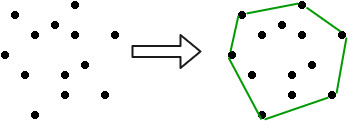
\includegraphics [width=\textwidth]{bab1/img/ilustrasi-convex-hull}
	\caption {Ilustrasi Convex Hull}
	\label {fig:ilustrasi-convex-hull}
\end{figure}
\par \textit{Relative convex hull} merupakan penurunan dari \textit{convex hull}. \textit{Relative convex hull} merupakan \textit{convex hull} yang mempunyai \textit{cavity} (cekungan ke dalam) yang diakibatkan atau relatif terhadap sesuatu yang membatasi \textit{convex hull} tersebut. Ilustrasi \textit{relative convex hull} dapat dilihat pada gambar \ref{fig:ilustrasi-relative-convex-hull}.

\begin{figure}[!h]
	\Centering
	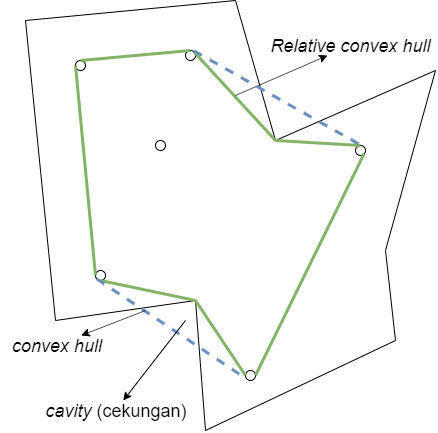
\includegraphics [width=0.5\columnwidth]{bab2/img/ilustrasi-relative-convex-hull}
	\caption {Ilustrasi Relative Convex Hull}
	\label {fig:ilustrasi-relative-convex-hull}
\end{figure}

\par Pada topik Tugas Akhir ini akan dijelaskan algoritma penyelesaian untuk mencari \textit{relative convex hull} dari sekumpulan titik yang berada di dalam sebuah polygon sederhana dengan menggunakan reduksi polygon pada studi kasus pada Sphere Online Judge 5637 LL and ErBao.

\section {Rumusan Masalah}

Rumusan masalah yang diangkat dalam Tugas Akhir ini adalah sebagai berikut :

\begin {enumerate}
    \item Bagaimana mencari \RCH dari kumpulan titik di dalam sebuah polygon?
    \item Bagaimana reduksi polygon menyelesaikan masalah \RCH dari kumpulan titik?
\end {enumerate}

\section {Batasan Masalah}
\label{sec:batasan_masalah}
Permasalahan yang dibahas pada Tugas Akhir ini memiliki beberapa batasan, yaitu sebagai berikut :
\begin{enumerate}
    \item Implementasi reduksi polygon sebagai penyelesaian permasalahan \RCH pada soal ISUN1.
    \item Algoritma \RCH terbatas pada analisis intuitif yang logis.
\end{enumerate}
Berikut merupakan batasan pada situs Sphere Online Judge: 
\begin {enumerate}
    \item Implementasi dilakukan menggunakan bahasa pemrograman C++.
    \item Banyaknya sisi pada polygon pembatas ($n$) diantara 3 sampai 500.
    \item Banyaknya pohon yang berada dalam taman ($m$) diantara 0 sampai 500.
    \item Batas maksimum untuk tiap vertex memenuhi($ x $, $ y $) dimana nilai |$x$|, |$y$| $\leq 10000$. 
    \item Banyak soal tidak diketahui karena program berhenti sampai EOF.
    \item Batas waktu yang diberikan adalah $ 0.142 $ detik.
    \item Batas memori yang diberikan adalah $ 1.536 $ MB.
    \item Batas kode sumber yang diberikan adalah $ 50.000 $ B. 
\end {enumerate}

\section {Tujuan}
Tujuan Tugas Akhir ini adalah sebagai berikut :
\begin{enumerate}
    \item Mengevaluasi kinerja reduksi polygon untuk menyelesaikan permasalahan komputasi \textit{relative convex hull} pada LL and ErBao.
\end{enumerate}

\section {Manfaat}
Tugas Akhir ini mampu memberikan pemahaman algoritma yang tepat untuk menyelesaikan permasalahan komputasi \textit{relative convex hull} dengan efisien.

\section {Metodologi}
Metodologi pengerjaan yang digunakan pada Tugas Akhir ini memiliki beberapa tahapan. Tahapan-tahapan tersebut yaitu :

\begin{enumerate}
    \item Penyusunan proposal\\
    Pada tahapan ini penulis memberikan penjelasan mengenai apa yang penulis akan lakukan dan mengapa Tugas Akhir ini dilakukan. Penjelasan tersebut dituliskan dalam bentuk proposal Tugas Akhir.
    \item Studi literatur\\
    Pada tahapan ini penulis mengumpulkan referensi yang diperlukan guna mendukung pengerjaan Tugas Akhir. Referensi yang digunakan dapat berupa hasil penelitian yang sudah pernah dilakukan, buku, artikel internet, atau sumber lain yang bisa dipertanggungjawabkan.
    \item Implementasi algoritma\\
    Pada tahapan ini penulis mulai mengembangkan algoritma yang digunakan untuk menyelesaikan permasalahan komputasi \textit{relative convex hull}.
    \item Pengujian dan evaluasi\\
    Pada tahapan ini penulis menguji performa algoritma yang digunakan. Hasil pengujian kemudian dievaluasi untuk kemudian dipertimbangkan apakah algoritma masih bisa ditingkatkan lagi atau tidak.
    \item Penyusunan buku\\
    Pada tahapan ini penulis menyusun hasil pengerjaan Tugas Akhir mengikuti format penulisan Tugas Akhir.
\end{enumerate}

\section {Sistematika Penulisan}
Sistematika laporan Tugas Akhir yang akan digunakan adalah sebagai berikut :
\begin{enumerate}
    \item BAB I : PENDAHULUAN\\
    Bab ini berisi latar belakang, rumusan masalah, batasan masalah, tujuan, manfaat, metodologi dan sistematika penulisan Tugas Akhir.
    \item BAB II : DASAR TEORI\\
    Bab ini berisi dasar teori mengenai permasalahan dan algoritma penyelesaian yang digunakan dalam Tugas Akhir
    \item BAB III : DESAIN\\
    Bab ini berisi desain algoritma dan struktur data yang digunakan dalam penyelesaian permasalahan.
    \item BAB IV : IMPLEMENTASI\\
    Bab ini berisi implementasi berdasarkan desain algoritma yang telah dilakukan pada tahap desain.
    \item BAB V : UJI COBA DAN EVALUASI\\
    Bab ini berisi uji coba dan evaluasi dari hasil implementasi yang telah dilakukan pada tahap implementasi.
    \item BAB VI : PENUTUP\\
    Bab ini berisi kesimpulan dan saran yang didapat dari hasil uji coba yang telah dilakukan.
\end{enumerate} \cleardoublepage
		\chapter {DASAR TEORI}

Pada bab ini, akan dijelaskan dasar teori yang digunakan sebagai landasaan pengerjaan Tugas Akhir ini.

\section{Deskripsi Permasalahan}
Permasalahan yang dibahas pada Tugas Akhir ini adalah perhitungan untuk mencari nilai $x$ yang didefinisikan oleh persamaan \eqref{eq:perimeter-polygon}.
\begin{equation}
    \label{eq:perimeter-polygon}
    x=\sum_{i=0}^{n-1} \text{RCH}_i
\end{equation}
$\text{RCH}_i$ pada persamaan \eqref{eq:perimeter-polygon} menyatakan sisi polygon dari RCH yang merupakan \textit{relative convex hull} yang didapatkan dari sekumpulan titik yang dibatasi di dalam polygon sederhana\cite{isun1}. Permasalahan pada tugas akhir ini adalah mencari \textit{relative convex hull} dari sekumpulan titik yang dibatasi oleh polygon sederhana. Gambar \ref{fig:ilustrasi-contoh-kasus-tanpa-solusi} dan \ref{fig:ilustrasi-contoh-kasus} merupakan contoh dari permasalahan ISUN1.
\begin{figure}
	\Centering
	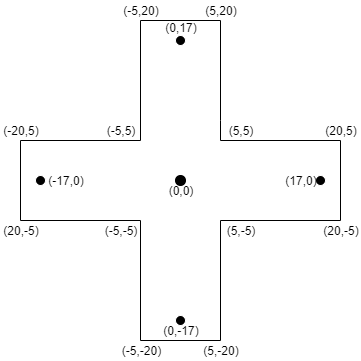
\includegraphics [width=0.5\columnwidth]{bab2/img/contoh-kasus-tanpa-solusi}
	\caption {Ilustrasi contoh kasus tanpa solusi}
	\label {fig:ilustrasi-contoh-kasus-tanpa-solusi}
\end{figure}
\begin{figure}
	\Centering
	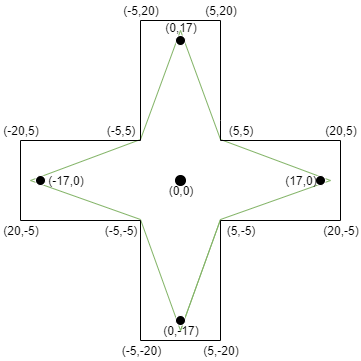
\includegraphics [width=0.5\columnwidth]{bab2/img/contoh-kasus}
	\caption {Ilustrasi contoh kasus}
	\label {fig:ilustrasi-contoh-kasus}
\end{figure}

\section{Convex Polygon}
Merupakan sebuah polygon sederhana yang memiliki sudut maksimal 180 derajat pada tiap edgenya. \textit{Convex polygon} memiliki beberapa properti, yaitu:
\begin{enumerate}
    \item sebuah garis lurus yang di gambar melewati sebuah \textit{convex} polygon akan berpotongan maksimal 2 kali. Ilustrasi dapat dilihan pada gambar \ref{fig:ilustrasi-properti-convex-polygon-1}
    \item Jika dua titik sembarang diambil dan ditarik garis antara keduanya, tidak ada bagian dari garis yang berada di luar polygon. Ilustrasi dapat dilihan pada gambar \ref{fig:ilustrasi-properti-convex-polygon-2}
\end{enumerate}
\begin{figure}
    \Centering
    
\includegraphics[width=0.5\columnwidth]{bab2/img/ilustrasi-properti-convex-polygon-1}
    \caption{Ilustrasi Properti Convex Polygon 1}
    \label{fig:ilustrasi-properti-convex-polygon-1}
\end{figure}
\begin{figure}
    \Centering
    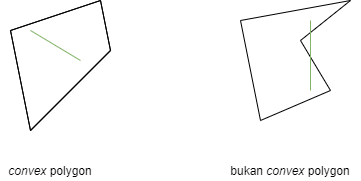
\includegraphics[width=0.5\columnwidth]{bab2/img/ilustrasi-properti-convex-polygon-2}
    \caption{Ilustrasi Properti Convex Polygon 2}
    \label{fig:ilustrasi-properti-convex-polygon-2}
\end{figure}

\subsection{Relative Convex Polygon}
Merupakan penurunan dari convex Polygon tetapi ada beberapa sisi dari polygon tersebut berbentuk convace atau cekung kedalam dikarenakan adanya batasan dari luar seperti polygon atau segmen garis lainnya. Ilustrasi relative convex polygon dapat dilihat pada gambar \ref{fig:ilustrasi-relative-convex-polygon}.
\begin{figure}
    \Centering
    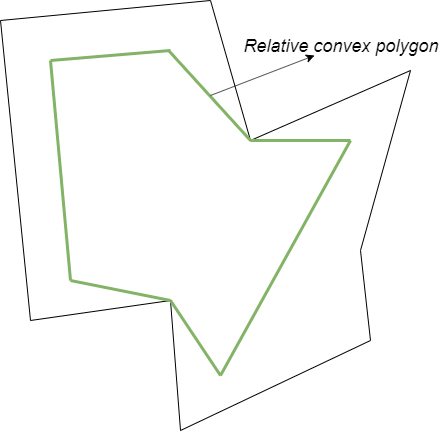
\includegraphics[width=0.5\columnwidth]{bab2/img/ilustrasi-relative-convex-polygon}
    \caption{Ilustrasi Relative Convex Polygon}
    \label{fig:ilustrasi-relative-convex-polygon}
\end{figure}
\section{Strategi Penyelesaian Permasalahan}
Pada subbab ini akan dipaparkan mengenai strategi penyelesaian masalah klasik pada daring SPOJ dengan kode ISUN1 menggunakan algoritma reduksi poligon. Secara singkat, strategi penyelesaian masalah dari ISUN1 menggunakan algoritma reduksin poligon menjadi 2 bagian besar yaitu :
\begin{enumerate}
    \item Pemrosesan titik pembentuk polygon yang membentuk \textit{Convex}.
    \item \textit{Convex Hull} dari titik yang berada didalam polygon
\end{enumerate}
Sebagai contoh, pada subbab ini akan menggunakan $P$ sebagai poligon luar yang mempunyai $n$ vertex, dimana $P = \left \langle p_1, p_2, ..., p_n \right \rangle$ yang mempunyai titik sebanyak $m$ ($S = \left \langle s_1, s_2, ..., s_m \right \rangle$), dan $D(A)$ merupakan sebuah deque (\textit{doubly-ended queue}) yang menampung vertex dari polygon $P$. Reduksi polygon didasari dari algoritma Melkman dengan sedikit modifikasi. Modifikasi yang dilakukan adalah ketika 3 buak titik pembentuk poligon yang konsekutif membuat \textit{convex} maka titik tengan dari ketiga titik tersebut dibuang, dan jika \textit{concave} maka titik tengahnya tetap disimpan. Pada saat sebuah titik dibuang, maka luas dari polygon akan tereduksi. Langkah - langkah reduksi dilakukan dengan mengulangi 2 langkah yang akan dijelaskan pada subbab \ref{sec:pemrosesan-titik-pembentuk-polygon-yang-membentuk-convex} dan \ref{sec:convex-hull-dari-titik-yang-berada-di-dalam-polygon}


\subsection{Pemrosesan Titik Pembentuk Polygon yang Membentuk Convex}
\label{sec:pemrosesan-titik-pembentuk-polygon-yang-membentuk-convex}
Pemrosesan titik pembentuk poligon dapat dilakukan dengan cara melakukan \textit{traversing} terhadap semua vertex pembentuk poligon. Untuk setiap vertex $p_i$ yang di cek, hitung orientasi(secara berlawanan jarum jam) titik $p_i$ dengan $p_{i-1}$ dan $ p_{i+1}$. Jika orientasinya membentuk \textit{convex} maka titik $p_i$ akan dibuang.
\par Sebelum membuang titik $p_i$, kita akan membuat sebuah segitiga $ABC$ dimana $A=p_i$, $B=p_{i-1}$, dan $C=p_{i+1}$ karena triangulation of polygon(Teorema \ref{theo:triangulation-of-polygon}).
\begin{theo}[Triangulation of Polygon]
    \label{theo:triangulation-of-polygon}
	Semua polygon dapat di buat dari beberapa segitiga.
\end{theo}
Kemudian cari $T(ABC)$ dimana $T(ABC)$ merupakan semua titik $S$ yang berada di dalam segitiga $ABC$ dengan menggunakan algoritma \textit{Point inside Polygon} (dapat dilihat pada subbab \ref{sec:point-inside-polygon}). Pencarian titik yang berada di dalam segitiga $ABC$ berguna untuk mencari pengganti vertex $p_i$ sebagai pembentuk poligon luarnya.

\subsection{Convex Hull dari Titik yang Berada di Dalam Polygon}
\label{sec:convex-hull-dari-titik-yang-berada-di-dalam-polygon}
Melanjutkan dari subbab \ref{sec:pemrosesan-titik-pembentuk-polygon-yang-membentuk-convex}, ketika sudah mendapatkan $T$, lakukan pencarian \textit{Convex Hull} dari titik - titik tersebut menggunakan \textit{monotone chain} (dapat dilihat pada subbab \ref{sec:algoritma-monotone-chain}). Kemudian sisipkan semua titik yang membentuk \textit{Convex Hull} diantara vertex $p_{i-1}$, $p_{i+1}$ untuk me-rekonstruksi poligon luar yang sudah di reduksi.

\section{Convex Hull}
\label{sec:convex-hull}
\textit{Convex Hull} dari sekumpulan titik $S$ adalah sebuah set dari semua kombinasi \textit{convex} dari titik - titik tersebut. Setiap titik $s_i$ pada $S$ diberikan sebuah koefisien $a_i$ dimana $a_i$ merupakan bialangan non negatif dan jika semua $a_i$ dijumlahkan hasilnya satu. Dan koefisien ini digunakan untuk menghitung berat rata - rata untuk setiap titik. Untuk setiap koefisien yang dipilih akan dikombinasikan dan menghasilkan \textit{convex hull}. Set \textit{convex hull} ini dapat di ekspresikan dengan formula \eqref{eq:convex-hull} dan ilustrasi \textit{convex hull} ada pada gambar \ref{fig:ilustrasi-convex-hull}.

\begin{equation}
    \label{eq:convex-hull}
    Conv(S)=\left\{ \sum_{i=1}^{|S|}{a_is_i} \big | (\forall{i}:a_i \ge 0 \wedge \sum_{i=1}^{|S|}{a_i=1} ) \right\}
\end{equation}
\begin{figure}
	\Centering
	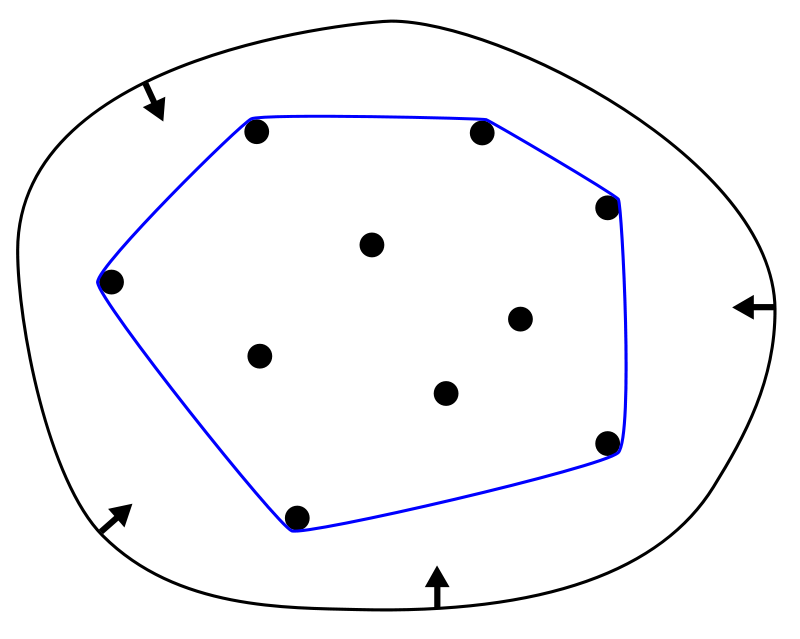
\includegraphics [width=0.5\columnwidth]{bab2/img/ilustrasi-convex-hull}
	\caption {Ilustrasi Convex Cull}
	\label {fig:ilustrasi-convex-hull}
\end{figure}


\subsection{Relative Convex Hull}
\textit{Relative convex hull} merupakan penurunan dari \textit{convex hull}. \textit{Relative convex hull} merupakan \textit{convex hull} yang mempunyai \textit{cavity} (cekungan kedalam) yang diakibatkan atau relatif terhadap sesuatu yang membatasi \textit{convex hull tersebut}. ilustrasi \textit{relative convex hull} dapat dilihat pada gambar \ref{fig:ilustrasi-relative-convex-hull}.

\begin{figure}
	\Centering
	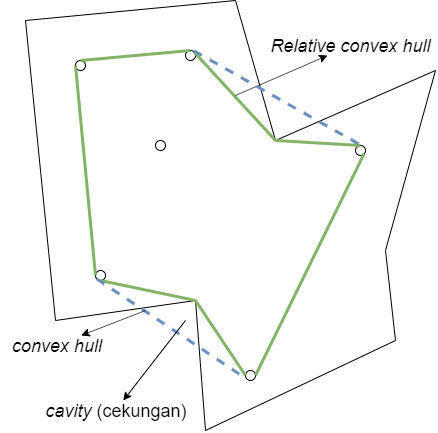
\includegraphics [width=0.5\columnwidth]{bab2/img/ilustrasi-relative-convex-hull}
	\caption {Ilustrasi Relative Convex Hull}
	\label {fig:ilustrasi-relative-convex-hull}
\end{figure}
\par Penentuan untuk mengetahui sebuah polygon merupakan \textit{convex} atau \textit{concave} dapat menggunakan orientasi. Apabila orientasi dari tiga titik yang berurutan adalah positif berlawanan jarum jam maka tiga titik tersebut adalah \textit{convex}. Sebaliknya apabila negatif maka tiga titik tersebut adalah \textit{concave}. Untuk mencari orientasi antara tiga titik dapat digunakan persamaan \ref{eq:orientasi}.
\begin{equation}
    \begin{aligned}
    \label{eq:orientasi}
        \vec{u}&=(B_x-A_x)x +(B_y-A_y)y\\
        \vec{v}&=(C_x-A_x)x +(C_y-A_y)y\\
    \end{aligned}
\end{equation}
$$ Orientasi = u_x*v_y - u_y*v_x $$
\subsection{Algoritma Convex Hull}
Ada beberapa algoritma yang dapat digunakan untuk mencari sebuah \textit{convex hull}, untuk melihat perbandingan dari beberapa algoritma dapat dilihat pada tabel \ref{tab:tabel-algoritma-convex-hull}.
\begin{table}[]
    \Centering
    \newcolumntype{P}[1]{>{\centering\arraybackslash}p{#1}}
    \caption{Tabel Perbandingan Algoritma Convex Hull}
    \label{tab:tabel-algoritma-convex-hull}
    \begin{tabular}{|P{2cm}|P{2cm}|P{2cm}|P{1.5cm}|P{2cm}|}
        \hline
    Algoritma Convex Hull & Implementasi & Kompleksitas & Kode Sumber     & Jenis Input \\ \hline
    Jarvis's Algorithm    & Mudah                  & $\mathcal{O}(n^2)$         & Singkat         & Kumpulan Titik\\ \hline
    Graham's Scan         & Sedikit Mudah          & $\mathcal{O}(n\log(n))$  & Singkat         & Kumpulan Titik  \\ \hline
    Quick Hull            & Kompleks               & $\mathcal{O}(n\log(n))$  & Panjang         & Kumpulan Titik  \\ \hline
    Monotone Chain        & Mudah                  & $\mathcal{O}(n\log(n))$  & Singkat         & Kumpulan Titik  \\ \hline
    Melkman's Algorithm   & Mudah                  & $\mathcal{O}(n)$           & Singkat         & Poligon Sederhana \\ \hline    
    \end{tabular}
\end{table}
Berdasarkan tabel \ref{tab:tabel-algoritma-convex-hull}, penulis memilih 2 algoritma yang akan digunakan pada buku ini.
\subsubsection{Algoritma Melkman Convex Hull}
\label{sec:algoritma-melkman-convex-hull}
Merupakan algoritma untuk menghitung rantai polygonal ataupun polygon sederhana dengan waktu linear $\mathcal{O}(n)$\cite{melkman_algorithm}. Asumsikan sebuah poligon sederhana $P$, dengan vertex $p_i$ dan edge $p_i p_{i+1}$. Algoritma ini menggunakan deque, $D = \left \langle d_1, d_2, ..., d_n \right \rangle$, untuk mereprentasikan \CH, $Q_i = CH(P_i)$, dimana $P_i = (p_0, p_1, ..., p_i)$. Deque mempunyai fungsi \textit{push} dan \textit{pop} dari atas/depan dan \textit{insert} dan \textit{remove} dari bawah/belakang. Secara spesifiknya yang dilakukan \textit{push} $v$ ke deque melakukan $(l \leftarrow l+1; d_t \leftarrow v)$, untuk \textit{pop} $d_t$ dari deque melakukan $(t \leftarrow t-1)$, untuk insert $v$ ke deque melakukan $(b \leftarrow b-1; d_b \leftarrow v)$, dan \textit{remove} $d_b$ dari deque melakukan $(b \leftarrow b+1)$.
\par Algoritma ini menggunakan konvensi dimana vertexnya berurutan secara berlawanan jarum jam di sekitar \CH $Q$.
\par Setiap $d_t$ dan $d_b$ mengacu kepada vertex yang sama pada rantai polygon $C$, dan vertex ini akan selalu menjadi vertex yang kita tambahkan terakhir pada \CH. Pseudocode Melkman Convex Hull dapat dilihat pada pseudocode \ref{psdo:Melkman-Convex-Hull}.
\begin{figure}
	\Centering
	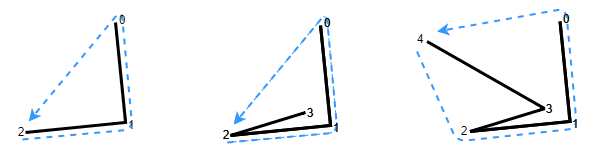
\includegraphics [width=\columnwidth]{bab2/img/ilustrasi-algoritma-melkman}
	\caption {Ilustrasi Algoritma Melkman}
	\label {fig:ilustrasi-algoritma-melkman}
\end{figure}
\begin{algorithm}
	\caption{Melkman Convex Hull}
	\label{psdo:Melkman-Convex-Hull}
	\begin{algorithmic}[1]
		\Require $P$
		\Ensure $Q$
        \State Inisialisasi: $D$
        \If{\fakesc{Left}($p_0, p_1, p_2$)}
            \State$D \leftarrow \left \langle p_2, p_0, p_1, p_2 \right \rangle$
        \Else
            \State $D \leftarrow \left \langle p_2, p_1, p_0, p_2 \right \rangle$
        \EndIf
        \State $i=3$
        \While{$i<n$}
            \While{ \fakesc{Left}($d_{t-1}, d_t, p_i$) dan \fakesc{Left}($d_b, d_{b+1}, p_i$))} 
                \State $i \leftarrow i+1$
            \EndWhile
            \While{!\fakesc{Left}($d_{t-1}, d_t, p_i$)}
                \State \textit{pop} $d_t$
            \EndWhile
            \State \textit{push} $p_i$
            \While{!\fakesc{Left}($p_i,d_{b}, d_{b+1}$)}
                \State \textit{remove} $d_b$
            \EndWhile
            \State \textit{insert} $p_i$
            \State $i \leftarrow i+1$
        \EndWhile
	\end{algorithmic}
\end{algorithm}

\subsubsection{Algoritma Monotone Chain}
\label{sec:algoritma-monotone-chain}
Algoritma \MC merupakan proses pembentukan \CH dari sekumpulan titik dengan kompleksitas $\mathcal{O}(n$ log$(n))$\cite{monotone_chain_algorithm}. Asumsikan sekumpulan titik $S$ sejumlah $n$ ,$S = \left \langle s_1, s_2, ..., s_n\right \rangle$ algoritma ini menggunakan list untuk membentuk sebuah rantai (\textit{monotone chain}), dimana list $L(S)$ menampung semua titik yang ada di $S$ yang terurut berdasarkan nilai koordinatnya terhadap sumbu $x$. algoritma ini memeriksa setiap 3 vertex yang berurutan, jika 3 vertex tersebut membuat \textit{convex} makan ketiga vertex tersebut disimpan, dan sebaliknya jika ketiga vertex tersebut membuat \textit{concave} maka vertex ke 2 akan dibuang dari vertex penyusun \textit{convex hull}. lalu lakukan hal yang sama dengan membalikan urutan pada $L$ untuk mendapatkan \textit{lower hull}. Pseudocode algoritma \textit{Monotone Chain} dapat dilihat pada pseudocode \ref{psdo:Monotone-Chain-Algorithm}.

\begin{figure}
	\Centering
	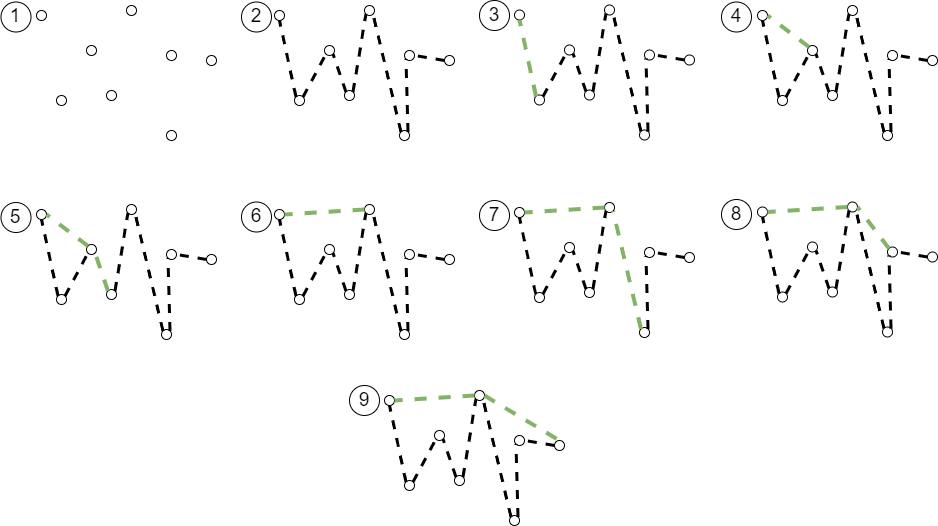
\includegraphics [width=\columnwidth]{bab2/img/ilustrasi-algoritma-monotone-chain}
	\caption {Ilustrasi Algoritma Monotone Chain}
	\label {fig:ilustrasi-algoritma-monotone-chain}
\end{figure}

\begin{algorithm}
	\caption{Monotone Chain Algorithm}
	\label{psdo:Monotone-Chain-Algorithm}
	\begin{algorithmic}[1]
		\Require $S$
		\Ensure $CH(S)$
        \State Inisialisasi: $L$
        \State Sort $S$
        \State $L \leftarrow S$
        \State Inisialisasi $CH(S)$
        \For{$i=0;i<2;i++$}
            \For{$j=0;j<Size(L);j++$}
                \While{$Size (CH)\ge2$ and $right(CH[Size(CH)-1],CH[Size(CH)-2],S[j])$}
                    \State Delete $CH$ last element
                \EndWhile
                \State push $pt$ to $CH$
            \EndFor
            \State reverse $L$
        \EndFor
	\end{algorithmic}
\end{algorithm}
\section{Point Inside Polygon}
\label{sec:point-inside-polygon}
\textit{Point Inside Polygon} merupakan algoritma untuk menentukan apakah suatu polygon berada di dalam sebuah polygon atau tidak \cite{point_inside_polygon}. Ide utama dari algoritma ini adalah dengan cara menarik garis sejajar dengan sumbu $x$ dimana garis tersebut berujung pada titik yang ingin dicari lokasinya kemudian hitung ada berapa edge dari poligon yang berpotongan dengan garis tersebut. Jika jumlah edge polygon yang berpotongan adalah ganjil, maka titik tersebut berada dalam polygon, dan sebaliknya, jika jumlahnya genap maka titik tersebut berada di luar polygon.

\begin{figure}
	\Centering
	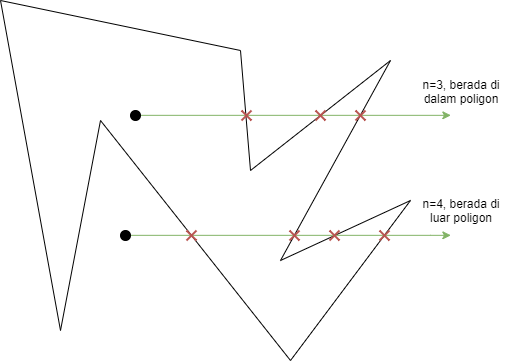
\includegraphics [width=0.5\columnwidth]{bab2/img/ilustrasi-algoritma-point-inside-polygon}
	\caption {Ilustrasi Algoritma Point Inside Polygon}
	\label {fig:ilustrasi-algoritma-point-inside-polygon}
\end{figure}
 \cleardoublepage
		\chapter{DESAIN}
\label{sec:desain}
Pada bab ini akan dijelaskan desain algoritma yang akan digunakan untuk menyelesaikan permasalahan.

\section{ Desain Umum Sistem}
\label{sec:desain-umum-sistem}
Pada subbab ini akan dijelaskan mengenai gambaran secara umum dari algoritma yang dirancang. Sistem diawali dengan menerima masukan 2 buah bilangan bulat $N$ yang merupakan banyaknya vertex pembentuk polygon luar dan $M$ yang merupakan banyaknya titik yang ada di dalam polygon tersebut. $N$ baris berikutnya berisikan 2 buah bilangan bulat $x_i$, $y_i$ yang merupakan koordinat dari vertex pembentuk polygon luar terurut berlawanan arah jarum jam. $M$ baris berikutnya berisikan dua buah bilangan bulat $x1_i$, $y1_i$ yang merupakan koordinat dari titik yang ada di dalam polygon.

\subsection{ Desain Fungsi Main}
Fungsi \fakesc{main} merupakan fungsi yang bertanggung jawab untuk menerima masukan yang sudah dijelaskan pada \ref{sec:desain-umum-sistem} untuk dilakukan proses selanjutnya. Pseudocode fungsi \fakesc{main} dapat dilihat pada pseudocode \ref{psdo:fungsi-main}. Fungsi \fakesc{Input} merupakan fungsi untuk menerima masukan, dan fungsi \fakesc{Print} merupakan fungsi untuk menampilkan hasil. 

\begin{algorithm}
	\caption{Fungsi \fakesc{main}}
	\label{psdo:fungsi-main}
    \begin{algorithmic}[1]
        \While{($N \leftarrow $ \fakesc{Input()}) and $N \neq EOF$}
            \State $M \leftarrow$ \fakesc{Input()}
            \State $perimeter \leftarrow$ \fakesc{Polygon}
            \State $trees \leftarrow$ Array \fakesc{Point}   
            \For {$i \leftarrow 1, N$}
                \State $x_i , y_i \leftarrow $ \fakesc{Input()}
                \State $perimeter.P[i]\leftarrow$ \fakesc{Point}($x_i$, $y_i$, false)
			\EndFor
			\If{$M=1$ or $M=0$}
				\State \fakesc{Print}($0$)
				\State \fakesc{Continue}
			\EndIf
            \For {$i \leftarrow 1, M$}
                \State $ x1_i , y1_i \leftarrow $ \fakesc{Input()}
                \State $trees \leftarrow$ \fakesc{Point}($x1_i$, $y1_i$, true)
            \EndFor
            \State $ans \leftarrow $\fakesc{Solve}($perimeter$, $trees$)
            \State \fakesc{Print} ($ans $)
        \EndWhile
	\end{algorithmic}
\end{algorithm}
\subsection{ Desain Class Point}
\label{sec:point}
Class \fakesc{Point} adalah class untuk menyimpan titik dalam diagram Kartesius. Pseudocode \ref{psdo:class-point} merupakan pseudocode dari class \fakesc{Point}. Nantinya pada implementasi, class ini akan melakukan \textit{override} terhadap operator perbandingan.
\begin{table}[htb]
	\Centering
	\caption{Nama dan Fungsi Variabel dalam Class \fakesc{Point}}
	\begin{tabular}{|c|p{7cm}|}
	\hline
	Nama Variabel & \multicolumn{1}{c|}{Fungsi Variabel}                               \\ \hline
$x$           & Menyimpan ordinat dari titik tersebut  \\ \hline
$y$           & Menyimpan absis dari titik tersebut          \\ \hline
$fixed$             & Untuk membedakan antara titik pembentuk polygon $P$ dan titik yang ada di dalam kumpulan titik $S$   \\ \hline
	\end{tabular}
	\label{tab:var-point}
\end{table}
\begin{algorithm}
	\caption{Class \fakesc{Point}}
	\label{psdo:class-point}
	\begin{algorithmic}[1]
        \State $ x, y \leftarrow $ \textbf{double}
        \State $fixed \leftarrow $ \textbf{boolean}
		\State \textbf{constructor} \Call{\fakesc{Point}}{$ $}
        \State \textbf{constructor} \Call{\fakesc{Point}}{$ \_x, \_y, \_fixed $}
	\end{algorithmic}
\end{algorithm}

Class \fakesc{Point} tidak memiliki fungsi karena class ini memang hanya untuk menyimpan suatu titik yang akan digunakan nanti.

Fungsi \textit{Constructor} dari class ini terdiri dari dua jenis. Fungsi \textit{constructor} yang pertama adalah fungsi dengan tanpa parameter, pada \textit{constructor} ini, semua variabel yang ada di dalam class \fakesc{Point} akan di inisialisasi dengan $0$. Fungsi \textit{constructor} kedua adalah fungsi dengan parameter $\_x, \_y, \_fixed$, menyatakan nilai $x, y, fixed$ secara berurutan.

\subsection{ Desain Class Vec}
\label{sec:vec}
Class \fakesc{Vec} merupakan class yang menyimpan vector dari dua buah titik pada diagram kartesian. Pseudocode \ref{psdo:class-vec} merupakan pseudocode dari class \fakesc{Vec}. 

\begin{table}[htb]
	\Centering
	\caption{Nama dan Fungsi Variabel dalam Class \fakesc{Vec}}
	\begin{tabular}{|c|p{7cm}|}
	\hline
	Nama Variabel & \multicolumn{1}{c|}{Fungsi Variabel}                               \\ \hline
$x$           & Menyimpan arah vektor absis  \\ \hline
$y$           & Menyimpan arah vektor ordinat          \\ \hline
	\end{tabular}
	\label{tab:var-vec}
\end{table}
\begin{algorithm}
	\caption{Class \fakesc{Vec}}
	\label{psdo:class-vec}
	\begin{algorithmic}[1]
        \State $ x, y \leftarrow $ \textbf{double}
		\State \textbf{constructor} \Call{\fakesc{Vec}}{$ $}
        \State \textbf{constructor} \Call{\fakesc{Vec}}{$ \_x, \_y $}
        \State \textbf{constructor} \Call{\fakesc{Vec}}{$ A, B $}
	\end{algorithmic}
\end{algorithm}

Class \fakesc{Vec} tidak memiliki fungsi karena class ini hanya untuk menyimpan vector dari dua titik yang akan digunakan nanti.

Fungsi \textit{Constructor} dari class ini terdiri dari 3 jenis. Fungsi \textit{constructor} yang pertama adalah fungsi dengan tanpa parameter, pada \textit{constructor} ini, semua variabel yang ada di dalam class \fakesc{Vec} akan di inisialisasi dengan $0$. Fungsi \textit{constructor} kedua adalah fungsi dengan parameter $\_x, \_y$, menyatakan nilai $x, y$ secara berurutan. Fungsi \textit{constructor} ketiga adalah fungsi dengan parameter $A, B$, menyatakan \fakesc{Point} dari titik $A$ dan \fakesc{Point} dari titik $B$, dimana nantinya nilai $x$ dan $y$ akan didapatkan dari pengurangan koordinat dari \fakesc{Point} $A$ dan \fakesc{Point} $B$.

\subsection{ Desain Class Line}
\label{sec:line}
Class \fakesc{Line} merupakan class yang bertanggung jawab untuk melakukan operasi-operasi pada garis dalam diagram kartesian. Pseudocode \ref{psdo:class-line} merupakan pseudocode dari Class \fakesc{Line}. 

\begin{table}[htb]
	\Centering
	\caption{Nama dan Fungsi Variabel dalam class \fakesc{Line}}
	\begin{tabular}{|c|p{7cm}|}
	\hline
	Nama Variabel & \multicolumn{1}{c|}{Fungsi Variabel}                               \\ \hline
$a$           & Menyimpan nilai $a$ pada persamaan $ax + by + c =0$ \\ \hline
$b$           & Menyimpan nilai $b$ pada persamaan $ax + by + c =0$          \\ \hline
$c$           & Menyimpan nilai $c$ pada persamaan $ax + by + c =0$          \\ \hline
	\end{tabular}
	\label{tab:var-line}
\end{table}
\begin{algorithm}
	\caption{Class \fakesc{Line}}
	\label{psdo:class-line}
	\begin{algorithmic}[1]
        \State $ a, b, c \leftarrow $ \textbf{double}
		\State \textbf{constructor} \Call{\fakesc{Line}}{$ $}
        \State \textbf{constructor} \Call{\fakesc{Line}}{$ \_a, \_b, \_c $}
        \State \textbf{constructor} \Call{\fakesc{Line}}{$ A, B $}
	\end{algorithmic}
\end{algorithm}

Class \fakesc{Line} tidak memiliki fungsi karena class ini hanya untuk menyimpan nilai dari fungsi $ax+by+c=0$ yang akan digunakan nanti.

Fungsi \textit{Constructor} dari class ini terdiri dari 3 jenis. Fungsi \textit{constructor} yang pertama adalah fungsi dengan tanpa parameter, pada \textit{constructor} ini, semua variabel yang ada di dalam class \fakesc{Line} akan di inisialisasi dengan $0$. Fungsi \textit{constructor} kedua adalah fungsi dengan parameter $\_a, \_b, \_c$, menyatakan nilai $a, b, c$ secara berurutan. Fungsi \textit{constructor} ketiga adalah fungsi dengan parameter $A, B$, menyatakan \fakesc{Point} dari titik $A$ dan \fakesc{Point} dari titik $B$, dimana nantinya nilai $a$, $b$ dan $c$ akan didapatkan dengan mencari fungsi garis yang melewati \fakesc{Point} $A$ dan \fakesc{Point} $B$.

\subsection{ Desain Class Segment}
\label{sec:segment}
Class \fakesc{Segment} merupakan class yang bertanggung jawab untuk menyimpan dan melakukan operasi-operasi pada segmen garis dalam diagram kartesian. Pseudocode \ref{psdo:class-segment} merupakan pseudocode dari class \fakesc{Segment}. 

\begin{table}[htb]
	\Centering
	\caption{Nama dan Fungsi Variabel dalam Class \fakesc{Segment}}
	\begin{tabular}{|c|p{7cm}|}
	\hline
	Nama Variabel & \multicolumn{1}{c|}{Fungsi Variabel}                               \\ \hline
$P$           & Menyimpan \fakesc{Point} yang merupakan ujung awal dari sebuah segmen garis \\ \hline
$Q$           & Menyimpan \fakesc{Point} yang merupakan ujung akhir dari sebuah segmen garis          \\ \hline
$L$           & Menyimpan fungsi dari garis yang melalui dua titik tersebut      \\ \hline
	\end{tabular}
	\label{tab:var-segment}
\end{table}
\begin{algorithm}
	\caption{Class \fakesc{Segment}}
	\label{psdo:class-segment}
	\begin{algorithmic}[1]
        \State $ P, Q \leftarrow $ \fakesc{Point}
        \State $L \leftarrow$ \fakesc{Line}
		\State \textbf{constructor} \Call{\fakesc{Segment}}{$ $}
        \State \textbf{constructor} \Call{\fakesc{Segment}}{$ \_P, \_Q$}
	\end{algorithmic}
\end{algorithm}

Class \fakesc{Segment} tidak memiliki fungsi karena class ini hanya untuk menyimpan data dari sebuah segmen garis yang akan digunakan nanti.

Fungsi \textit{Constructor} dari class ini terdiri dari 2 jenis. Fungsi \textit{constructor} yang pertama adalah fungsi dengan tanpa parameter, pada \textit{constructor} ini, semua variabel yang ada di dalam class \fakesc{Segment} akan di inisialisasi dengan $0$. Fungsi \textit{constructor} kedua adalah fungsi dengan parameter $\_P, \_Q$, menyatakan \fakesc{Point} dari titik $P$ dan \fakesc{Point} dari titik $Q$, yang merupakan titik \fakesc{Point} $A$ dan \fakesc{Point} $B$ secara berturut, dan \fakesc{Line} $L$ didapar dengan menggunakan \textit{constructor} \fakesc{Line} dengan parameter $P$ dan $Q$.

\subsection{ Desain Class Polygon}
\label{sec:polygon}
Class \fakesc{Polygon} merupakan class yang bertanggung jawab untuk menyimpan dan melakukan operasi-operasi pada polygon pada diagram kartesian. Pseudocode \ref{psdo:class-polygon} merupakan pseudocode dari class \fakesc{Polygon}. 

\begin{table}[htb]
	\Centering
	\caption{Nama dan Fungsi Variabel dalam Class \fakesc{Polygon}}
	\begin{tabular}{|c|p{7cm}|}
	\hline
	Nama Variabel & \multicolumn{1}{c|}{Fungsi Variabel}                               \\ \hline
$P$           & Menyimpan array dari \fakesc{Point} yang membentuk polygon tersebut \\ \hline
	\end{tabular}
	\label{tab:var-polygon}
\end{table}
\begin{algorithm}
	\caption{Class \fakesc{Polygon}}
	\label{psdo:class-polygon}
	\begin{algorithmic}[1]
        \State $ P \leftarrow $ Array \fakesc{Point}
		\State \textbf{constructor} \Call{\fakesc{Polygon}}{$ $}
        \State \textbf{constructor} \Call{\fakesc{Polygon}}{$ \_P$}
        \State \textbf{function} \Call{\fakesc{prev}}{$ idx $}
		\State \textbf{function} \Call{\fakesc{next}}{$ idx $}
		\State \textbf{function} \Call{\fakesc{perimeter}}{$ $}
	\end{algorithmic}
\end{algorithm}

Fungsi-fungsi yang terkandung dalam class ini adalah \fakesc{prev}, \fakesc{next}, \fakesc{perimeter}. Tabel \ref{tab:var-polygon} menjelaskan variabel dan kegunaannya dalam class \fakesc{Polygon}. 

Fungsi \textit{Constructor} dari class ini terdiri dari 2 jenis. Fungsi \textit{constructor} yang pertama adalah fungsi dengan tanpa parameter, pada \textit{constructor} ini, variabel $P$ yang ada di dalam class \fakesc{Polygon} akan di inisialisasi. Fungsi \textit{constructor} kedua adalah fungsi dengan parameter $\_P$, menyatakan array \fakesc{Point} dari titik pembentuk polygon tersebut.

Fungsi \textit{next} bertanggung jawab untuk mencari index selanjutnya dari titik yang membentuk polygon. Masukan, proses dan keluaran dari fungsi ini tercantum pada tabel \ref{tab:class-polygon-next}. Pseudocode fungsi ini dapat dilihat pada pseudocode \ref{psdo:class-polygon-next}.

\begin{table}[htb]
	\Centering
	\caption{Masukan, Proses, dan Keluaran dari Fungsi \fakesc{Next} Class \fakesc{Polygon}}
	\begin{tabular}{|p{3cm}|p{3cm}|p{3cm}|}
	\hline
	Masukan   & Proses     & Keluaran \\ \hline
	Suatu bilangan bulat $idx$ yang menyatakan index saat ini & mencari index selanjutnya &   Suatu bilangan bulat yang menyatakan index selanjutnya     \\ \hline
	\end{tabular}
	\label{tab:class-polygon-next}
\end{table}

\begin{algorithm}
    \caption{Fungsi \fakesc{Next} pada class \fakesc{Polygon}}
	\label{psdo:class-polygon-next}
	\begin{algorithmic}[1]
        \Require $ idx $
        \If{$idx = $\fakesc{Size}($P$)$-1$}
            \State \Return $0$
        \Else
            \State \Return $idx+1$
		\EndIf
	\end{algorithmic}
\end{algorithm}

Fungsi \textit{prev} bertanggung jawab untuk mencari index sebelumnya dari titik yang membentuk polygon. Masukan, proses dan keluaran dari fungsi ini tercantum pada tabel \ref{tab:class-polygon-prev}. Pseudocode fungsi ini dapat dilihat pada pseudocode \ref{psdo:class-polygon-prev}.

\begin{table}[htb]
	\Centering
	\caption{Masukan, Proses, dan Keluaran dari Fungsi \fakesc{Prev} Class \fakesc{Polygon}}
	\begin{tabular}{|p{3cm}|p{3cm}|p{3cm}|}
	\hline
	Masukan   & Proses     & Keluaran \\ \hline
	Suatu bilangan bulat $idx$ yang menyatakan index saat ini & mencari index sebelumnya &   Suatu bilangan bulat yang menyatakan index sebelumnya     \\ \hline
	\end{tabular}
	\label{tab:class-polygon-prev}
\end{table}

\begin{algorithm}
    \caption{Fungsi \fakesc{Prev} pada class \fakesc{Polygon}}
	\label{psdo:class-polygon-prev}
	\begin{algorithmic}[1]
        \Require $ idx $
        \If{$idx = 0$}
            \State \Return \fakesc{Size}($P$)$-1$
        \Else
            \State \Return $idx-1$
		\EndIf
	\end{algorithmic}
\end{algorithm}

Fungsi \textit{perimeter} bertanggung jawab untuk mencari keliling dari sebuah polygon. Masukan, proses, dan keluaran dari fungsi ini tercantum pada tabel \ref{tab:class-polygon-perimeter}. Pseudocode fungsi ini dapat dilihat pada pseudocode \ref{psdo:class-polygon-perimeter}.
\begin{table}[htb]
	\Centering
	\caption{Masukan, Proses, dan Keluaran dari Fungsi \fakesc{Perimeter} Class \fakesc{Polygon}}
	\begin{tabular}{|p{3cm}|p{3cm}|p{3cm}|}
	\hline
	Masukan   & Proses     & Keluaran \\ \hline
	- & Mencari keliling dengan mencari jarak eulerian dari semua titik pembentuk polygon &   Suatu bilangan berkoma yang menyatakan keliling dari polygon tersebut     \\ \hline
	\end{tabular}
	\label{tab:class-polygon-perimeter}
\end{table}

\begin{algorithm}
    \caption{Fungsi \fakesc{Perimeter} pada class \fakesc{Polygon}}
	\label{psdo:class-polygon-perimeter}
    \begin{algorithmic}[1]
        \State $ret \leftarrow 0$
        \For{$i \leftarrow 0$ \textbf{to} \fakesc{Size}($P$)$-1$}
            \State $ret \leftarrow ret $ \fakesc{EDist}($P[i]$, $P[$ \fakesc{next}($i$)$] $)
        \EndFor
        \State \Return $ret$
	\end{algorithmic}
\end{algorithm}

\subsection{ Desain Fungsi BetweenD}
\label{sec:fungsi-betweend}
Fungsi \fakesc{BetweenD} bertanggung jawab untuk mencari tahu apakah suatu bilangan $x$ berada diantara bilangan $l$ dan bilangan$r$. Pseudocode dari fungsi \fakesc{BetweenD} dapat dilihat pada pseudocode \ref{psdo:fungsi-betweend}. Masukan, proses, dan keluaran dari fungsi ini tercantum pada tabel \ref{tab:fungsi-betweend}.

\begin{table}[htb]
	\Centering
	\caption{Masukan, Proses, dan Keluaran dari Fungsi \fakesc{BetweenD} }
	\begin{tabular}{|p{3cm}|p{3cm}|p{3cm}|}
	\hline
	Masukan   & Proses     & Keluaran \\ \hline
	Tiga buah bilangan $x,l,r$, dimana bilangan $x$ merupakan bilangan yang ingin diketahui apakah berada diantara titik $l$ dan $r$ & Mencari tahu apakah bilangan $x$ berada diantara bilangan $l$ dan $r$ &   Sebuah boolean yang menyatakan apakah $x$ berada diantara $l$ dan $r$     \\ \hline
	\end{tabular}
	\label{tab:fungsi-betweend}
\end{table}
\begin{algorithm}
    \caption{Fungsi \fakesc{BetweenD}}
	\label{psdo:fungsi-betweend}
    \begin{algorithmic}[1]
        \Require $x, l, r$
        \If{\fakesc{Min}($l, r$) $\le x + EPS$ and $x \le$ \fakesc{Max}($l, r$) $+ EPS$}
            \State \Return \fakesc{True}
        \Else
            \State \Return \fakesc{False}
        \EndIf
	\end{algorithmic}
\end{algorithm}


\subsection{ Desain Fungsi EDist}
\label{sec:fungsi-edist}
Fungsi \fakesc{EDist} bertanggung jawab untuk mencari jarak antara dua titik \fakesc{Point} $A$ dan \fakesc{Point} $B$ dengan menggunakan rumus \textit{Pythagoras}. Rumus \textit{Pythagoras} dapat di lihat pada persamaan \ref{eq:pythagoras}. Pseudocode fungsi \fakesc{EDist} dapat dilihat pada pseudocode \ref{psdo:fungsi-edist}. Masukan, proses, dan keluaran dari fungsi ini tercantum pada tabel \ref{tab:fungsi-edist}.

\begin{equation}
    \label{eq:pythagoras}
    C=\sqrt{A^2 + B^2}
\end{equation}

\begin{table}[htb]
	\Centering
	\caption{Masukan, Proses, dan Keluaran dari Fungsi \fakesc{EDist} }
	\begin{tabular}{|p{3cm}|p{3cm}|p{3cm}|}
	\hline
	Masukan   & Proses     & Keluaran \\ \hline
	Dua buah \fakesc{Point} $A$ dan \fakesc{Point} $B$ yang akan dicari jaraknya & Mencari jarak antara \fakesc{Point} $A$ dan \fakesc{Point} $B$ &   Sebuah bilangan berkoma yang menyatakan jarak \fakesc{Point} $A$ dan \fakesc{Point} $B$  \\ \hline
	\end{tabular}
	\label{tab:fungsi-edist}
\end{table}

\begin{algorithm}
    \caption{Fungsi \fakesc{EDist}}
	\label{psdo:fungsi-edist}
    \begin{algorithmic}[1]
        \Require $A, B$
        \State \Return \fakesc{Sqrt}($(A*A)+(B*B)$)
	\end{algorithmic}
\end{algorithm}

\subsection{ Desain Fungsi Cross}
\label{sec:fungsi-cross}
Fungsi \fakesc{Cross} bertanggung jawab untuk mencari nilai perkalian \textit{cross} dari dua buah vector. Rumus Pythagoras dapat di lihat pada persamaan \ref{eq:cross}. Pseudocode fungsi \fakesc{Cross} dapat dilihat pada pseudocode \ref{psdo:fungsi-cross}. Masukan, proses, dan keluaran dari fungsi ini tercantum pada tabel \ref{tab:fungsi-cross}.

\begin{equation}
    \label{eq:cross}
    C = (u_x*v_y) - (u_y*v_x)
\end{equation}
\begin{table}[htb]
	\Centering
	\caption{Masukan, Proses, dan Keluaran dari Fungsi \fakesc{Cross} }
	\begin{tabular}{|p{3cm}|p{3cm}|p{3cm}|}
	\hline
	Masukan   & Proses     & Keluaran \\ \hline
	Dua buah \fakesc{Vec} $U$ dan \fakesc{Vec} $V$ yang akan dicari hasil perkalian silangnya & Mencari nilai perkalian silang dari \fakesc{Vec} $U$ dan \fakesc{Vec} $V$ &   Sebuah bilangan yang menyatakan hasil perkalian silang \fakesc{Vec} $U$ dan \fakesc{Vec} $V$  \\ \hline
	\end{tabular}
	\label{tab:fungsi-cross}
\end{table}


\begin{algorithm}
    \caption{Fungsi \fakesc{Cross}}
	\label{psdo:fungsi-cross}
    \begin{algorithmic}[1]
        \Require $U, V$
        \State \Return $(U.x*V.y) - (U.y*V.x)$
	\end{algorithmic}
\end{algorithm}

\subsection{ Desain Fungsi Orientation}
\label{sec:fungsi-orientation}
Fungsi \fakesc{Orientation} bertanggung jawab untuk mencari orientasi dari tiga titik. Pseudocode fungsi \fakesc{Orientation} dapat dilihat pada pseudocode \ref{psdo:fungsi-orientation}. Masukan, proses, dan keluaran dari fungsi ini tercantum pada tabel \ref{tab:fungsi-orientation}.

\begin{table}[htb]
	\Centering
	\caption{Masukan, Proses, dan Keluaran dari Fungsi \fakesc{Orientation} }
	\begin{tabular}{|p{3cm}|p{3cm}|p{3cm}|}
	\hline
	Masukan   & Proses     & Keluaran \\ \hline
	Tiga buah \fakesc{Point} $O$, \fakesc{Point} $P$ dan \fakesc{Point} $Q$ yang akan dicari orientasinya & Mencari orientasi antara \fakesc{Point} $O$, \fakesc{Point} $P$ dan \fakesc{Point} $Q$ &   Sebuah bilangan yang menyatakan orientasi antara \fakesc{Point} $O$, \fakesc{Point} $P$ dan \fakesc{Point} $Q$  \\ \hline
	\end{tabular}
	\label{tab:fungsi-orientation}
\end{table}
\begin{algorithm}
    \caption{Fungsi \fakesc{Orientation}}
	\label{psdo:fungsi-orientation}
    \begin{algorithmic}[1]
        \Require $O, P, Q$
        \State $OP \leftarrow$ \fakesc{Vec}($O,P$)
        \State $OQ \leftarrow$ \fakesc{Vec}($O,Q$)
        \State \Return \fakesc{Cross}($OP, OQ$)
	\end{algorithmic}
\end{algorithm}

\subsection{ Desain Fungsi OnSegment}
\label{sec:fungsi-onsegment}
Fungsi \fakesc{OnSegment} bertanggung jawab untuk mencari tahu apakah sebuah titik \fakesc{Point} $P$ bersentuhan dengan sebuah segmen garis \fakesc{Segment} $S$ atau tidak. Pseudocode fungsi \fakesc{OnSegment} dapat dilihat pada pseudocode \ref{psdo:fungsi-onsegment}. Masukan, proses, dan keluaran dari fungsi ini tercantum pada tabel \ref{tab:fungsi-onsegment}.

\begin{table}[htb]
	\Centering
	\caption{Masukan, Proses, dan Keluaran dari Fungsi \fakesc{OnSegment} }
	\begin{tabular}{|p{3cm}|p{3cm}|p{3cm}|}
	\hline
	Masukan   & Proses     & Keluaran \\ \hline
	Dua buah \fakesc{Point} $P$ dan \fakesc{Segment} $S$ yang akan dicari tahu apakah \fakesc{Point} $P$ berada di \fakesc{Segment} $S$ & Mencari tahu apakah \fakesc{Point} $P$ berada di \fakesc{Segment} $S$ &   Sebuah boolean yang menyatakan apakah \fakesc{Point} $P$ berada di dalam \fakesc{Segment} $S$ \\ \hline
	\end{tabular}
	\label{tab:fungsi-onsegment}
\end{table}
\begin{algorithm}
    \caption{Fungsi \fakesc{OnSegment}}
	\label{psdo:fungsi-onsegment}
    \begin{algorithmic}[1]
        \Require $P, S$
        \If{\fakesc{Orientation}($S.P, S.Q, P$)}
            \State \Return \fakesc{False}
        \Else
            \State \Return (\fakesc{BetweenD}($P.x, S.P.x, S.Q.x$) and \fakesc{BetweenD}($P.y, S.P.y, S.Q.y$))
        \EndIf
	\end{algorithmic}
\end{algorithm}

\subsection{ Desain Fungsi ConvexHull}
\label{sec:fungsi-convexhull}
Fungsi \fakesc{ConvexHull} bertanggung jawab untuk mencari \textit{convex hull} dari sekumpulan titik $pts$. Algoritma yang digunakan oleh fungsi ini adalah algoritma \textit{Monotone Chain} yang dapat dilihat pada bagian \ref{sec:algoritma-monotone-chain}. Pseudocode dari fungsi \fakesc{ConvexHull} yang digunakan dapat dilihat pada Pseudocode \ref{psdo:fungsi-convexhull}.  Masukan, proses, dan keluaran dari fungsi ini tercantum pada tabel \ref{tab:fungsi-convexhull}.

\begin{table}[htb]
	\Centering
	\caption{Masukan, Proses, dan Keluaran dari Fungsi \fakesc{ConvexHull} }
	\begin{tabular}{|p{3cm}|p{3cm}|p{3cm}|}
	\hline
	Masukan   & Proses     & Keluaran \\ \hline
    Sebuah array \fakesc{Point} $pts$ yang merupakan sekumpulan titik & Mencari \fakesc{Polygon} dengan keliling terkecil dari sekumpulan titik &   Sebuah \fakesc{Polygon} yang mengelilingi kumpulan \fakesc{Point} $pts$  \\ \hline
	\end{tabular}
	\label{tab:fungsi-convexhull}
\end{table}
\begin{algorithm}
    \caption{Fungsi \fakesc{ConvexHull}}
	\label{psdo:fungsi-convexhull}
    \begin{algorithmic}[1]
        \Require $pts$
        \State \fakesc{Sort}($pts$)
        \State $hull \leftarrow$ Array \fakesc{Point}
        \For{$i \leftarrow 0$ to $2$}
            \State $start \leftarrow$ \fakesc{Size}($hull$)
            \For{$pt$ in $pts$}
                \While{(\fakesc{Size}($hull$)$\ge start+2$) and (\fakesc{Orientation}($hull[$\fakesc{size}($hull$)$-1]$, $hull[$\fakesc{size}($hull$)$-2]$, $pt$)$\le 0$)}
                \State $hull.$\fakesc{Erase}($hull[$\fakesc{size}($hull$)$-1]$)
                \EndWhile
                \State $hull.$\fakesc{Insert}($pt$)
            \EndFor
            \State $hull.$\fakesc{Erase}($hull[$\fakesc{size}($hull$)$-1]$)
            \State \fakesc{reverse}($pts$)
        \EndFor
        \State \Return \fakesc{Polygon}($hull$);
	\end{algorithmic}
\end{algorithm}

\subsection{ Desain Fungsi InSimplePolygon}
\label{sec:fungsi-insimplepolygon}
Fungsi \fakesc{InSimplePolygon} bertanggung jawab untuk mencari tahu apakah sebuah titik \fakesc{Point} $P$ berada di dalam \fakesc{Polygon} $A$ atau tidak. Algoritma yang digunakan pada fungsi ini adalah algoritma \textit{point inside polygon} yang dapat dilihat pada bagian \ref{sec:point-inside-polygon}. Pada desain fungsi \fakesc{InSimplePolygon} ada 3 macam keluaran yaitu $-1$ untuk menandakan bahwa \fakesc{Point} $P$ berada di dalam \fakesc{Polygon} $A$, $0$ untuk menandakan bahwa \fakesc{Point} $P$ berada di salah satu sisi \fakesc{Polygon} $A$, dan $1$ untuk menandakan bahwa \fakesc{Point} $P$ berada di luar \fakesc{Polygon} $A$. Pseudocode fungsi \fakesc{InSimplePolygon} dapat dilihat pada pseudocode \ref{psdo:fungsi-insimplepolygon}. Masukan, proses, dan keluaran dari fungsi ini tercantum pada tabel \ref{tab:fungsi-insimplepolygon}.

\begin{table}[htb]
	\Centering
	\caption{Masukan, Proses, dan Keluaran dari Fungsi \fakesc{InSimplePolygon} }
	\begin{tabular}{|p{3cm}|p{3cm}|p{3cm}|}
	\hline
	Masukan   & Proses     & Keluaran \\ \hline
	Sebuah \fakesc{Point} $A$ dan sebuah \fakesc{Polygon} $P$ yang akan dicari tahu apakah \fakesc{Point} $A$ berada di dalam \fakesc{Polygon} $P$ & Mencari tahu apakah \fakesc{Point} $A$ berada di dalam \fakesc{Polygon} $P$ &   Sebuah bilangan yang apakah \fakesc{Point} $A$ berada di dalam \fakesc{Polygon} $P$  \\ \hline
	\end{tabular}
	\label{tab:fungsi-insimplepolygon}
\end{table}

\begin{algorithm}
    \caption{Fungsi \fakesc{InSimplePolygon}}
	\label{psdo:fungsi-insimplepolygon}
    \begin{algorithmic}[1]
        \Require $P, A$
        \State $ret \leftarrow$ \fakesc{Integer}
        \For{$i \leftarrow 0$ to \fakesc{Size}($A.P$)}
            \If{$P = A.P[i]$}
                \State \Return $0$
            \EndIf
            \State $j \leftarrow A.$\fakesc{Next}($i$)
            \If{\fakesc{OnSegment}($P$, \fakesc{Segment}($A.P[i], A.P[j]$))}
                \State \Return $0$
            \EndIf
            \State $below \leftarrow (A.P[i].y < P.y)$
            \If{$below \neq (A.P[j].y<P.y)$}
                \State $o \leftarrow$ \fakesc{Orientation}($P, A.P[i], A.P[j]$)
                \If{$o = 0$}
                    \State \Return $0$
                \EndIf
                \If{$below = (o>0)$ and $below =$ \fakesc{True}}
                    \State $ret+=1$
                \Else
                    \If{$below = (o>0)$ and $below =$ \fakesc{False}}
                        \State $ret-=1$
                    \EndIf
                \EndIf
            \EndIf
        \EndFor
        \If{$ret=0$}
            \State \Return $1$
        \Else
            \State \Return $-1$
        \EndIf
	\end{algorithmic}
\end{algorithm}

\newpage
\subsection{ Desain Fungsi GetBetween}
\label{sec:fungsi-getbetween}
Fungsi \fakesc{getBetween} bertanggung jawab untuk mencari list \fakesc{Point} yang akan menggantikan \fakesc{Point} yang akan dibuang. Pseudocode fungsi \fakesc{GetBetween} dapat dilihat pada pseudocode \ref{psdo:fungsi-getbetween}. Masukan, proses, dan keluaran dari fungsi ini tercantum pada tabel \ref{tab:fungsi-getbetween}.
\begin{table}[htb]
	\Centering
	\caption{Masukan, Proses, dan Keluaran dari Fungsi \fakesc{GetBetween} }
	\begin{tabular}{|p{3cm}|p{3cm}|p{3cm}|}
	\hline
	Masukan   & Proses     & Keluaran \\ \hline
	Sebuah \fakesc{Polygon} $triangle$ yang merupakan segitiga, \fakesc{Queue} \fakesc{Point} $q$ yang merupakan pembentuk polygon luar, dan array \fakesc{Point} $trees$ yang merupakan titik yang berada di dalam polygon luar & Mencari \fakesc{Point} mana saja yang akan menggantikan \fakesc{Point} $triangle[1]$ yang akan dibuang &   Sebuah \fakesc{List} \fakesc{Point} yang berisikan daftar \fakesc{Point} yang akan menggantikan \fakesc{Point} $triangle[1]$  \\ \hline
	\end{tabular}
	\label{tab:fungsi-getbetween}
\end{table}

\begin{algorithm}
    \caption{Fungsi \fakesc{GetBetween}}
	\label{psdo:fungsi-getbetween}
    \begin{algorithmic}[1]
        \Require $triangle, q, trees$
        \State $points,pts \leftarrow$ Array \fakesc{Point}
        \While{$q$ not \fakesc{Empty}}
            \If{\fakesc{InSimplepolygon}(q.\fakesc{front}(), $triangle$) $\neq 1$}
                \State $points.$\fakesc{Insert}($q.$\fakesc{Front}())
            \EndIf
            \State $q.$\fakesc{Pop}
        \EndWhile
        \For{$pt$ in $trees$}
            \If{\fakesc{InSimplepolygon}($pt$, $triangle$) $\neq 1$}
                \State $points.$\fakesc{Insert}($pt$)
            \EndIf
        \EndFor
        \State $P \leftarrow$ \fakesc{ConvexHull}($points$)
        \State $i \leftarrow 0$
        \While{\fakesc{True}}
            \If{$P.P[i]=triangle.P[0]$}
                \If{$P.P[P.$\fakesc{Next}($i$)$]=triangle.P[2]$}
                    \State $i \leftarrow P.$\fakesc{Prev}($i$)
                    \While{$P.P[i] \neq triangle.P[2]$}
                        \State $pts.$\fakesc{Insert}($P.P[i]$)
                        \State $i = P.$\fakesc{Prev}($i$)
                    \EndWhile
                \Else
                    \State $i \leftarrow P.$\fakesc{Next}($i$)
                    \While{$P.P[i] \neq triangle.P[2]$}
                        \State $pts.$\fakesc{Insert}($P.P[i]$)
                        \State $i = P.$\fakesc{Next}($i$)
                    \EndWhile
                \EndIf
                \State \fakesc{Break}
            \EndIf
            \State $i\leftarrow P.$\fakesc{Next}($i$)
        \EndWhile
        \State \Return $pts$
	\end{algorithmic}
\end{algorithm}
\newpage
\subsection{ Desain Fungsi Solve}
\label{sec:fungsi-solve}
Fungsi \fakesc{Solve} bertanggung jawab untuk mencari \textit{relative convex polygon} yang mengelilingi semua titik yang ada di dalam polygon luar. Pseudocode fungsi \fakesc{Solve} dapat dilihat pada pseudocode \ref{psdo:fungsi-solve}. Masukan, proses, dan keluaran dari fungsi ini tercantum pada tabel \ref{tab:fungsi-solve}.
\begin{table}[htb]
	\Centering
	\caption{Masukan, Proses, dan Keluaran dari Fungsi \fakesc{Solve} }
	\begin{tabular}{|p{3cm}|p{3cm}|p{3cm}|}
	\hline
	Masukan   & Proses     & Keluaran \\ \hline
	Sebuah \fakesc{Polygon} $perimeter$ yang merupakan polygon sederhana yang merupakan polygon pembatas, dan array \fakesc{Point} $trees$ yang merupakan titik yang berada di dalam polygon pembatas & Mencari \textit{relative convex hull} dari semua titik $trees$ di dalam \fakesc{Polygon} $perimeter$  &   Sebuah \fakesc{Polygon} yang merupakan \textit{relative convex hull} dari semua titik $trees$ \\ \hline
	\end{tabular}
	\label{tab:fungsi-solve}
\end{table}


\begin{algorithm}
    \caption{Fungsi \fakesc{Solve}}
	\label{psdo:fungsi-solve}
    \begin{algorithmic}[1]
        \Require $perimeter, trees$
        \State $q \leftarrow$ \fakesc{Queue}
        \For{$pt$ in $perimeter.P$} 
        \State $q.$\fakesc{Push} $pt$
		\EndFor
		\State $bef \leftarrow perimeter.P[perimeter.$\fakesc{Size}$()-1]$
		\While{\fakesc{True}}
			\State $erased \leftarrow$ \fakesc{False}
			\State $count \leftarrow q.$\fakesc{Size}()
			\While{count--}
				\State $cur \leftarrow q.$\fakesc{Front}()
				$q.$\fakesc{Pop}()
				\If{$cur.fixed =$\fakesc{False} and (\fakesc{Fine}($q,cur$) or $cur = bef$ or $cur = q.$\fakesc{Front}())}
					\State $erased \leftarrow$ \fakesc{True}
					\State $triangle \leftarrow$ \fakesc{Polygon}
					\State $triangle.P.$\fakesc{Insert}($bef, cur, q.$\fakesc{Front}())
					\State $points \leftarrow$ \fakesc{GetBetween}($triangle,q,trees$)
					\For{$pt$ in $points$}
						\State $q.$\fakesc{Push}($pt$);
						$bef \leftarrow pt$
					\EndFor
				\Else
					\State $q.$\fakesc{Push}($cur$);
					$bef \leftarrow cur$
				\EndIf
			\EndWhile
			\If{$erased =$ \fakesc{False}}
				\fakesc{Break}
			\EndIf
		\EndWhile  
		\State $hull \leftarrow$ array of \fakesc{Point}
		\While{$q$ not empty}
			\State $hull.$\fakesc{Insert}($q.$\fakesc{Front}())
			\State $q.$\fakesc{Pop}()
		\EndWhile
		\State \Return \fakesc{Polygon}($hull$)
	\end{algorithmic}
\end{algorithm}

\newpage
\section{ Desain Pembangkit Kasus Uji}
\label{sec:pembangkit-kasus-uji}
Pada subbab ini akan dijelaskan mengenai gambaran secara umum dari pembangkit kasus uji untuk melakukan uji coba lokal pada Tugas Akhir ini.
Sistem \fakesc{GenerateTestCase} bertanggung jawab untuk membuat kasus uji berdasarkan banyaknya titik yang ingin di uji. Pseudocode fungsi \fakesc{GenerateTestCase} dapat dilihat pada pseudocode \ref{psdo:pembangkit-kasus-uji}. Masukan, proses, dan keluaran dari fungsi ini tercantum pada tabel \ref{tab:pembangkit-kasus-uji}.
\begin{table}[htb]
	\Centering
	\caption{Masukan, Proses, dan Keluaran dari Fungsi \fakesc{GenerateTestCase} }
	\begin{tabular}{|p{3cm}|p{3cm}|p{3cm}|}
	\hline
	Masukan   & Proses     & Keluaran \\ \hline
	Sebuah bilangan bulat $N$ dan $M$ yang merupakan banyaknya vertex polygon dan banyaknya titik di dalam polygon & Membangun kasus uji sebanyak masukan  &   Sebuah polygon sederhana dan sekumpulan titik acak sebanyak $N$ yang berada di dalam polygon sederhana\\ \hline
	\end{tabular}
	\label{tab:pembangkit-kasus-uji}
\end{table}


\begin{algorithm}
    \caption{Fungsi \fakesc{GenerateTestCase}}
	\label{psdo:pembangkit-kasus-uji}
    \begin{algorithmic}[1]
        \Require $N, M$
        \State $polygon \leftarrow$ \fakesc{Array}
        \State $trees \leftarrow$ \fakesc{Array}
        \For{$i \leftarrow 0$ to $N/4$} 
        	\State $polygon.$\fakesc{Push} ([$-10000+(i*20000/N), -10000$])
		\EndFor
        \For{$i \leftarrow 0$ to $N/4$} 
        	\State $polygon.$\fakesc{Push} ([10000, $-10000+(i*20000/N)$])
		\EndFor
        \For{$i \leftarrow 0$ to $N/4$} 
        	\State $polygon.$\fakesc{Push} ([$10000-(i*20000/N), 10000$])
		\EndFor
        \For{$i \leftarrow 0$ to $N-3*N/4$} 
        	\State $polygon.$\fakesc{Push} ([$10000, 10000-(i*20000/N)$])
		\EndFor
        \For{$i \leftarrow 0$ to $N-3*N/4$} 
        	\State $trees.$\fakesc{Push} ([(\fakesc{Random}() mod $20001$)-$10000$,(\fakesc{Random}() mod $20001$)-$10000$])
		\EndFor
		\State \Return (N, M, polygon, trees)
	\end{algorithmic}
\end{algorithm} \cleardoublepage
	%	\chapter {IMPLEMENTASI}

\section{Lingkungan implementasi}

Lingkungan implementasi dan pengembangan yang dilakukan adalah sebagai berikut.
\begin{enumerate}
	\item Perangkat Keras
	\begin{enumerate}
		\item Processor Intel® Core™ i7-6500U CPU @ 2.50GHz (4 CPUs), ~2.6GHz
		\item Random Access Memory 8192MB
	\end{enumerate}
	\item Perangkat Lunak
	\begin{enumerate}
		\item Sistem Operasi Windows 10 Home Single Language 64-bit
		\item Dev C++
		\item Bahasa Pemrograman C++
		\item Kompiler GCC 7.4.0 (Ubuntu 7.4.0-1ubuntu1~18.04.1) untuk Windows Subsystem Linux
	\end{enumerate}
\end{enumerate}

\section{Implementasi Program Utama}

Subbab ini menjelaskan implementasi proses algoritma secara Keseluruhan berdasarkan desain yang telah dijelaskan pada Bab \ref{sec:desain}. Program ini merupakan program yang digunakan untuk menyelesaikan permasalahan \textit{LL and ErBao}.

\subsection{Header yang diperlukan}
Implementasi algoritma ini membutuhkan lima buah \textit{header} yaitu \texttt{iostream}, \texttt{vector}, \texttt{cmat}, \texttt{functional} dan \texttt{algorithm} seperti yang terlihat pada Kode Sumber \ref{code:header_main}.

\begin{code}[firstnumber=1]{\textit{Header} yang Diperlukan}{header_main}
#pragma GCC optimize("O3")
#pragma GCC target("avx")

#include <iostream>
#include<vector>
#include<cmath>
#include<map>
#include<queue>
#include<algorithm>
\end{code}

Selain header, terdapat juga preprocessor \textit{pragma}, digunakan untuk mengganti flag kompiler yang digunakan pada daring SPOJ.
\textit{Header} \texttt{iostream} berisi fungsi standar input output operasi yang digunakan oleh bahasa C++. \textit{Header} \texttt{vector} berisi struktur data yang digunakan untuk menyimpan data array secara dinamis. \textit{Header} \texttt{cmath} berisi fungsi-fungsi untuk operasi matematika seperti fungsi \texttt{hypot}. \textit{Header} \texttt{queue} berisi struktur data yang digunakan untuk menyimpan antrian data. \textit{Header} \texttt{algorithm} berisi modul yang memiliki fungsi-fungsii yang sangat berguna dalam membantu mengimplementasi algoritma yang telah dibangun, contohnya adalah fungsi \textit{reverse} dan \textit{sort}. \textit{Header} \texttt{map} berisi struktur data untuk menyimpan data \textit{key value}.

\subsection{Preprocessor}
Pre-processor seperti \texttt{using} digunakan untuk membuat alias dari tipe data sesungguhnya. Terdapat tiga alias yang digunakan yaitu \texttt{push\_back(x)} sebagai \texttt{pb(x)}, \texttt{pop\_back(x)} sebagai \texttt{pob(x)}, \texttt{getchar(x)} sebagai \texttt{gc(x)}, dan \texttt{for (int i = 0; i < n; i++)} sebagai \texttt{FOR(i,n)}. Pre-processor dapat dilihat pada Kode Sumber \ref{code:preprocessor_main}.

\begin{code}[firstnumber=1]{\textit{Preprocessor} yang Diperlukan}{preprocessor_main}
#define pb(x) push_back(x)
#define pob(x) pop_back(x)
#define FOR(i, n) for (int i = 0; i < n; i++)
#define gc(x) getchar(x)
using namespace std;
\end{code}

\subsection{Variabel Global}
Variabel global digunakan untuk memudahkan dalam mengakses data yang digunakan lintas fungsi/struct. Kode sumber implementasi variabel global dapat dilihat pada kode sumber \ref{code:var_glob_main}. Variabel tersebut didefinisikan secara global agar dapat digunakan pada setiap fungsi.

\begin{code}[firstnumber=1]{Variabel Global yang Didefinisikan Setelah Definisi Struct Mod64}{var_glob_main}
	
const double EPS = 0.0;
const double INF = 1E9;
map<point, int> pool;
\end{code}

\subsection{Implementasi Fungsi Main}
Fungsi main adalah implementasi algoritma yang dirancang pada pseudocode \ref{psdo:fungsi-main}. Implementasi fungsi main dapat dilihat pada Kode Sumber \ref{code:main}. 
\begin{code}[firstnumber=1]{Fungsi Main}{main}
int main(){
	int kase = 1;
	int n, m;
	while (cin >> n){
		pool.clear();
		cin >> m;
		polygon perimeter;
		vector<point> trees;

		for (int i = 0; i < n; i++){
			double a = readint(), b = readint();
			pool[point(a, b, false)]++;
			perimeter.P.push_back(point(a, b, false));
		}

		if (m == 0 || m == 1){
			printf("Case #%d: %.3lf\n", kase++, 0.0);
			continue;
		}

		for (int i = 0; i < m; i++){
			double a = readint(), b = readint();
			pool[point(a, b, true)]++;
			trees.push_back(point(a, b, true));
		}

		polygon hasil = solve(perimeter, trees);

		printf("Case #%d: %.3lf\n", kase++, hasil.perimeter());
	}
}
\end{code}

\subsection{Implementasi Class Point}
Pada subbab ini akan dijelaskan mengenai implementasi dari class \texttt{Point} pada subbab \ref{sec:point} dan pseudocode \ref{psdo:class-point}. Implementasi dari class \texttt{Point} dapat dilihat pada Kode Sumber \ref{code:class-point}.

\begin{code}[firstnumber=1]{Struct Point}{class-point}
struct point{
	double x, y;
	bool fixed;
	point(){
		x = y = 0.0;
		fixed = 0;
	}
	point(double _x, double _y, bool _fixed = false){
		x = _x;
		y = _y;
		fixed = _fixed;
	}
	bool operator<(point other) const{
		if (y < other.y + EPS)
			return true;
		if (y + EPS > other.y)
			return false;
		return x < other.x + EPS;
	}
	bool operator==(point other) const{
		return same_d(x, other.x) && same_d(y, other.y);
	}
};
\end{code}

\subsection{Implementasi Class Vec}
Pada subbab ini akan dijelaskan mengenai implementasi dari class \texttt{Vec} pada subbab \ref{sec:vec} dan pseudocode \ref{psdo:class-vec}. Implementasi dari class \texttt{Vec} dapat dilihat pada Kode Sumber \ref{code:class-vec}.

\begin{code}[firstnumber=1]{Struct Vec}{class-vec}
struct vec{
	double x, y;
	vec(){
		x = y = 0.0;
	}
	vec(double _x, double _y){
		x = _x;
		y = _y;
	}
	vec(point A){
		x = A.x;
		y = A.y;
	}
	vec(point A, point B){
		x = B.x - A.x;
		y = B.y - A.y;
	}
};
\end{code}

\subsection{Implementasi Class Line}
Pada subbab ini akan dijelaskan mengenai implementasi dari class \texttt{Line} pada subbab \ref{sec:line} dan pseudocode \ref{psdo:class-line}. Implementasi dari class \texttt{Line} dapat dilihat pada Kode Sumber \ref{code:class-line}.

\begin{code}[firstnumber=1]{Struct Line}{class-line}
struct line{
	double a, b, c;
	line(){
		a = b = c = 0.0;
	}
	line(double _a, double _b, double _c){
		a = _a;
		b = _b;
		c = _c;
	}
	line(point P1, point P2){
		if (P2 < P1){
			point T;
			T = P1;
			P1 = P2;
			P2 = T;
		}
		if (same_d(P1.x, P2.x))
			a = 1.0, b = 0.0, c = -P1.x;
		else
			a = -(P1.y - P2.y) / (P1.x - P2.x), b = 1.0, c = -(a * P1.x) - P1.y;
	}
	line(point P, double slope){
		if (same_d(slope, INF))
			a = 1.0, b = 0.0, c = -P.x;
		else
			a = -slope, b = 1.0, c = -(a * P.x) - P.y;
	}
	bool operator==(line other) const{
		return same_d(a, other.a) && same_d(b, other.b) && same_d(c, other.c);
	}
};
\end{code}

\subsection{Implementasi Class Segment}
Pada subbab ini akan dijelaskan mengenai implementasi dari class \texttt{Segment} pada subbab \ref{sec:segment} dan pseudocode \ref{psdo:class-segment}. Implementasi dari class \texttt{Segment} dapat dilihat pada Kode Sumber \ref{code:class-segment}.

\begin{code}[firstnumber=1]{Struct Segment}{class-segment}
struct segment{
	point P, Q;
	line L;
	segment(){
		point T1;
		P = Q = T1;
		line T2;
		L = T2;
	}
	segment(point _P, point _Q){
		if (_Q < _P){
			point T1 = _P;
			_P = _Q;
			_Q = T1;
		}
		P = _P;
		Q = _Q;
		line T2(_P, _Q);
		L = T2;
	}
	bool operator==(segment other) const{
		return P == other.P && Q == other.Q;
	}
};
\end{code}

\subsection{Implementasi Class Polygon}
Pada subbab ini akan dijelaskan mengenai implementasi dari class \texttt{Polygon} pada subbab \ref{sec:polygon} dan pseudocode \ref{psdo:class-polygon}. Implementasi dari class \texttt{Polygon} dapat dilihat pada Kode Sumber \ref{code:class-polygon}.

\begin{code}[firstnumber=1]{Struct Polygon}{class-polygon}
struct polygon{
	vector<point> P;
	polygon(){
		P.clear();
	}
	polygon(vector<point> &_P){
		P = _P;
	}
	int prev(int idx){
		return (idx == 0 ? P.size() - 1 : idx - 1);
	}
	int next(int idx){
		return (idx == P.size() - 1 ? 0 : idx + 1);
	}
	double perimeter(){
		double ret = 0;
		FOR(i, P.size()){
			ret += e_dist(P[i], P[next(i)]);
		}
		return ret;
	}
};
\end{code}

\subsection{Implementasi Fungsi BetweenD}
Pada subbab ini akan dijelaskan mengenai implementasi dari fungsi \texttt{BetweenD} pada pseudocode \ref{psdo:fungsi-betweend}. Implementasi dapat dilihat pada Kode Sumber \ref{code:fungsi-betweend}.

\begin{code}[firstnumber=1]{Fungsi BetweenD}{fungsi-betweend}
double between_d(double x, double l, double r){
	return (min(l, r) <= x + EPS && x <= max(l, r) + EPS);
}
\end{code}

\subsection{Implementasi Fungsi EDist}
Pada subbab ini akan dijelaskan mengenai implementasi dari fungsi \texttt{EDist} pada pseudocode \ref{psdo:fungsi-edist}. Implementasi dapat dilihat pada Kode Sumber \ref{code:fungsi-edist}.

\begin{code}[firstnumber=1]{Fungsi EDist}{fungsi-edist}
double e_dist(point P1, point P2){
	return hypot(P1.x - P2.x, P1.y - P2.y);
}
\end{code}

\subsection{Implementasi Fungsi Cross}
Pada subbab ini akan dijelaskan mengenai implementasi dari fungsi \texttt{Cross} pada pseudocode \ref{psdo:fungsi-cross}. Implementasi dapat dilihat pada Kode Sumber \ref{code:fungsi-cross}.

\begin{code}[firstnumber=1]{Fungsi Cross}{fungsi-cross}
double cross(vec u, vec v){
	return (u.x * v.y - u.y * v.x);
}
\end{code}

\subsection{Implementasi Fungsi Orientation}
Pada subbab ini akan dijelaskan mengenai implementasi dari fungsi \texttt{Orientation} pada pseudocode \ref{psdo:fungsi-orientation}. Implementasi dapat dilihat pada Kode Sumber \ref{code:fungsi-orientation}.

\begin{code}[firstnumber=1]{Fungsi Orientation}{fungsi-orientation}
double orientation(point O, point P, point Q){
	vec OP(O, P), OQ(O, Q);
	double c = cross(OP, OQ);
	return c;
}
\end{code}

\subsection{Implementasi Fungsi OnSegment}
Pada subbab ini akan dijelaskan mengenai implementasi dari fungsi \texttt{OnSegment} pada pseudocode \ref{psdo:fungsi-onsegment}. Implementasi dapat dilihat pada Kode Sumber \ref{code:fungsi-onsegment}.

\begin{code}[firstnumber=1]{Fungsi OnSegment}{fungsi-onsegment}
bool onSegment(point P, segment S){
	if (orientation(S.P, S.Q, P) != 0.0)
		return false;
	return between_d(P.x, S.P.x, S.Q.x) && between_d(P.y, S.P.y, S.Q.y);
}
\end{code}

\subsection{Implementasi Fungsi ConvexHull}
Pada subbab ini akan dijelaskan mengenai implementasi dari fungsi \texttt{ConvexHull} pada pseudocode \ref{psdo:fungsi-convexhull}. Implementasi dapat dilihat pada Kode Sumber \ref{code:fungsi-convexhull}.

\begin{code}[firstnumber=1]{Fungsi ConvexHull}{fungsi-convexhull}
polygon convexHull(vector<point> &pts){
	sort(pts.begin(), pts.end());
	vector<point> hull;
	for (int i = 0; i < 2; i++){
		int start = (int)hull.size();
		for (int i = 0; i < pts.size(); i++){
			point pt = pts[i];
			while ((int)hull.size() >= start + 2 && orientation(hull[(int)hull.size() - 1], hull[(int)hull.size() - 2], pt) <= 0.0)
				hull.pob();
			hull.pb(pt);
		}
		hull.pop_back();
		reverse(pts.begin(), pts.end());
	}
	if ((int)hull.size() == 2 && hull[0] == hull[1])
		hull.pob();
	return polygon(hull);
}
\end{code}

\subsection{Implementasi Fungsi InSimplePolygon}
Pada subbab ini akan dijelaskan mengenai implementasi dari fungsi \texttt{inSimplePolygon} pada pseudocode \ref{psdo:fungsi-insimplepolygon}. Implementasi dapat dilihat pada Kode Sumber \ref{code:fungsi-insimplepolygon}.

\begin{code}[firstnumber=1]{Fungsi InSimplePolygon}{fungsi-insimplepolygon}
int inSimplePolygon(point P, polygon &A){
	int ret = 0;
	FOR(i, A.P.size()){
		if (P == A.P[i])
			return 0;
		int j = A.next(i);
		if (onSegment(P, segment(A.P[i], A.P[j])))
			return 0;
		bool below = (A.P[i].y < P.y);
		if (below != (A.P[j].y < P.y)){
			double o = orientation(P, A.P[i], A.P[j]);
			if (o == 0.0)
				return 0;
			if (below == (o > 0.0))
				ret += below ? 1 : -1;
		}
	}
	return ret == 0 ? 1 : -1;
}
\end{code}

\subsection{Implementasi Fungsi GetBetween}
Pada subbab ini akan dijelaskan mengenai implementasi dari fungsi \texttt{GetBetween} pada pseudocode \ref{psdo:fungsi-getbetween}. Implementasi dapat dilihat pada Kode Sumber \ref{code:fungsi-getbetween}.

\begin{code}[firstnumber=1]{Fungsi GetBetween}{fungsi-getbetween}
vector<point> getBetween(polygon &triangle, queue<point> q, vector<point> trees){
	vector<point> points;

	while (!q.empty()){
		if (inSimplePolygon(q.front(), triangle) != 1){
			points.pb(q.front());
		}
		q.pop();
	}
	for (int i = 0; i < trees.size(); i++){
		if (inSimplePolygon(trees[i], triangle) != 1){
			points.pb(trees[i]);
		}
	}

	polygon P = convexHull(points);

	vector<point> pts;
	int i = 0;
	while (1){
		if (P.P[i] == triangle.P[0]){
			if (P.P[P.next(i)] == triangle.P[2]){
				i = P.prev(i);
				while (!(P.P[i] == triangle.P[2])){
					pts.pb(P.P[i]);
					i = P.prev(i);
				}
			}
			else{
				i = P.next(i);
				while (!(P.P[i] == triangle.P[2])){
					pts.pb(P.P[i]);
					i = P.next(i);
				}
			}
			break;
		}
		i = P.next(i);
	}
	return pts;
}	
\end{code}

\subsection{Implementasi Fungsi Solve}
Pada subbab ini akan dijelaskan mengenai implementasi dari fungsi \texttt{Solve} pada pseudocode \ref{psdo:fungsi-solve}. Implementasi dapat dilihat pada Kode Sumber \ref{code:fungsi-solve}.

\begin{code}[firstnumber=1]{Fungsi Solve}{fungsi-solve}
polygon solve(polygon &perimeter, vector<point> &trees){
	queue<point> q;
	for (int i = 0; i < perimeter.P.size(); i++){
		q.push(perimeter.P[i]);
	}

	point bef = perimeter.P[perimeter.P.size() - 1];
	while (1){
		bool erased = 0;
		int count = q.size();
		while (count--){
			point cur = q.front();
			q.pop();
			pool[cur]--;
			if (!cur.fixed && (!find(q, cur) || cur == bef || cur == q.front()) && orientation(cur, bef, q.front()) <= 0.0){
				erased = true;
				polygon triangle;
				triangle.P.pb(bef);
				triangle.P.pb(cur);
				triangle.P.pb(q.front());
				vector<point> points = getBetween(triangle, q, trees);
				for (int i = 0; i < points.size(); i++){
					q.push(points[i]);
					pool[points[i]]++;
					bef = points[i];
				}
			}
			else{
				q.push(cur);
				pool[cur]++;
				bef = cur;
			}
		}
		if (!erased)
			break;
	}

	vector<point> hull;
	while (!q.empty()){
		hull.pb(q.front());
		q.pop();
	}
	return polygon(hull);
}
\end{code} \cleardoublepage
	%	\chapter{UJI COBA DAN EVALUASI}

Pada bab ini dijelaskan tentang uji coba dan evaluasi dari implementasi yang telah dilakukan pada tugas akhir ini.
\section{Lingkungan Uji Coba}
Lingkungan uji coba digunakan untuk uji coba kebenaran adalah salah satu sistem yang digunakan situs penilaian daring Sphere Online Judge, yaitu kluster \textit{Cube} dengan spesifikasi sebagai berikut :
\begin{enumerate}
	\item Perangkat Keras
	\begin{enumerate}
		\item Processor Intel Xeon E3-1220 v5 (5 CPUs)
		\item Random Access Memory 1536MB
	\end{enumerate}
	\item Perangkat Lunak
	\begin{enumerate}
		\item Kompiler GCC 6.3.0
	\end{enumerate}
\end{enumerate}

Lingkungan uji coba yang digunakan untuk melakukan uji coba kinerja menggunakan komputer pribadi penulis yang memiliki spesifikasi sebagai berikut
\begin{enumerate}
	\item Perangkat Keras
	\begin{enumerate}
		\item Processor Intel® Core™ i7-6500U CPU @ 2.50GHz (4 CPUs), ~2.6GHz
		\item Random Access Memory 8192MB
	\end{enumerate}
	\item Perangkat Lunak
	\begin{enumerate}
		\item Sistem Operasi Windows 10 Home Single Language 64-bit
		\item Visual Studio Code
		\item Bahasa Pemrograman C++
		\item Kompiler GCC 7.4.0 (Ubuntu 7.4.0-1ubuntu1~18.04.1) untuk Windows Subsystem Linux
	\end{enumerate}
\end{enumerate}

\section{Skenario Uji Coba}
\label{sec:skenario-uji-coba}
Subbab ini akan menjelaskan hasil pengujian program untuk menyelesaikan permasalahan LL and ErBao. Metode pengujian yang dilakukan adalah sebagai berikut.
\begin{enumerate}
	\item Pengujian luar. Pengujian ini menggunakan Online Judge untuk menguji kebenaran dan kinerja program.
	\item Pengujian lokal. Pengujian ini menggunakan mesin yang digunakan dalam pengembangan untuk mengukur kinerja program.
\end{enumerate}
Dalam pengujian lokal, dibuat beberapa kasus uji berdasarkan batasan yang ada pada soal.
\par Untuk pengujian luar, uji coba dilakukan dengan mengirimkan kode program dengan algoritma reduksi polygon ke situs penilaian daring Sphere Online Judge sebanyak 10 kali.

\section{Uji Coba Kebenaran}
Pada subbab ini akan dibahas mengenai uji coba kebenaran yang dilakukan dengan mengirim kode sumber terkait ke dalam situs penilaian daring Sphere Online Judge. Bukti hasil pengujian dapat dilihat pada gambar \ref{fig:hasil-uji-coba-kebenaran-situs-penilaian-spoj}.
\begin{figure}[!h]
	\Centering
	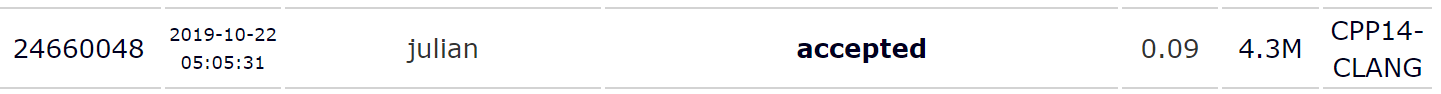
\includegraphics [width=\columnwidth]{bab5/img/hasil-uji-coba-kebenaran-situs-penilaian-spoj}
	\caption {Hasil Uji Coba Kebenaran Situs Penilaian Sphere Online Judge}
	\label {fig:hasil-uji-coba-kebenaran-situs-penilaian-spoj}
\end{figure}

\section{Uji Coba Kinerja Lokal}
Pada subbab ini akan ditampilkan hasil uji coba kinerja dari algoritma reduksi polygon untuk menyelesaikan permasalahan LL and ErBao. Pengujian dilakukan terhadap kelompok masukan yang telah dijelaskan pada subbab \ref{sec:skenario-uji-coba}. Detil masukan dapat dilihat pada Lampiran A. Langkah pengujian kinerja dilakukan dengan langkah sebagai berikut:
\begin{enumerate}
	\item Rekam waktu tepat sebelum komputasi penyelesaian masalah.
	\item Melakukan komputasi penyelesaian masalah untuk masukan kasus uji yang sama sebanyak 10 kali secara berturut-turut.
	\item Rekam waktu tepat setelah komputasi dengan mengurangi waktu selesai komputasi dengan waktu sebelum komputasi.
	\item Ulangi untuk semua kasus uji.
\end{enumerate}
\par Grafik \ref{fig:mean-running-time} menampilkan rata-rata kinerja masing-masing metode. Pada grafik tersebut dapat dilihat bahwa rata-rata \textit{running time} reduksi polygon dengan algoritma \textit{Melkman convex hull} berbanding lurus dengan banyaknya titik di dalam polygon tersebut.
\begin{figure}[!h]
	\Centering
	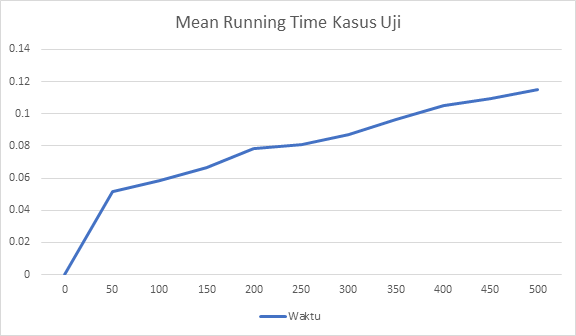
\includegraphics [width=\columnwidth]{bab5/img/mean-running-time}
	\caption {Grafik Mean Running Time Kasus Uji}
	\label {fig:mean-running-time}
\end{figure}

\section{Evaluasi Kebenaran Uji Coba Lokal}
Evaluasi dilakukan dengan memeriksa hasil keluaran program apakah sama dengan contoh keluaran pada Sphere Online Judge 5637 LL and ErBao. Tabel kebenaran dapat dilihat pada gambar \ref{tab:masukan-dan-keluaran-contoh-1}

\begin{table}[]
	\Centering
	\begin{tabular}{|l|c|}
	\hline
	\multicolumn{1}{|l|}{Data Masukan}  & Hasil Keluaran \\ \hline
	\begin{tabular}[l]{@{}l@{}}8 2\\ 0 0\\ 30 0\\ 30 20\\ 20 20\\ 20 10\\ 10 10\\ 10 20\\ 0 20\\ 5 15\\ 25 15\end{tabular} & Case \#1: 48.284          \\ \hline
	\end{tabular}
	\caption{Tabel Data Uji Coba Kebenaran Lokal dengan Sampel Data }
	\label{tab:masukan-dan-keluaran-contoh-1}
\end{table}

\par Gambar \ref{fig:kondisi-awal} menunjukan ilustrasi kondisi awal program sebelum iterasi dimulai.
\begin{figure}[!h]
	\Centering
	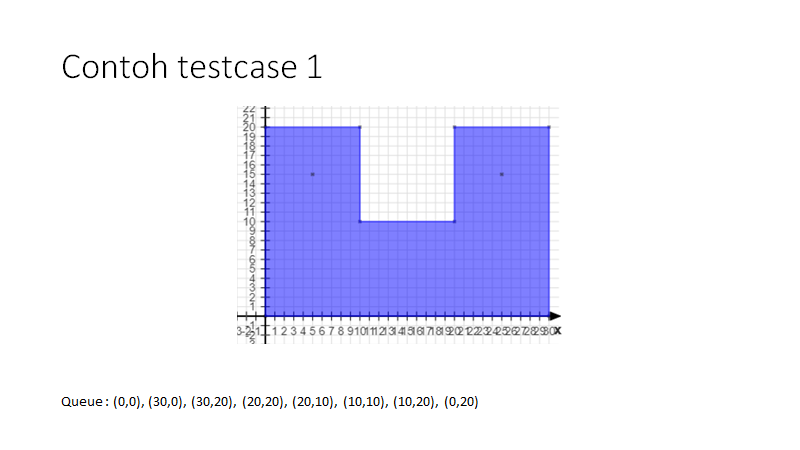
\includegraphics [width=\columnwidth]{bab5/img/kondisi-awal}
	\caption {Ilustrasi Kondisi Awal}
	\label {fig:kondisi-awal}
\end{figure}

\par Pada awal iterasi ke-1, memeriksa titik $(0,0)$. Titik tersebut akan dibuang karena titik tersebut merupakan titik luar dan orientasi terhadap titik sebelumnya dan sesudahnya membentuk \textit{convex}. Sebelum membuang titik tersebut, program membuat segitiga dengan titik sebelumnya, titik tersebut dan titik sesudahnya. Kemudian program mencari semua titik yang berada di dalam segitiga tersebut. Selanjutnya program mencari \textit{convex hull} dari semua titik yang didapatkan dan disisipkan ke queue polygon luar untuk menggantikan titik yang dibuang. Kondisi setelah iterasi ke-1 dapat dilihat pada gambar \ref{fig:iterasi-1}.
\begin{figure}[!h]
	\Centering
	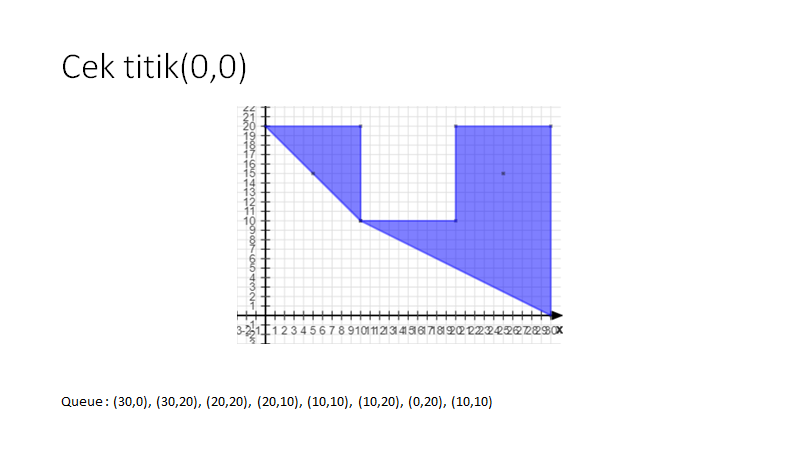
\includegraphics [width=\columnwidth]{bab5/img/iterasi-1}
	\caption {Ilustrasi Iterasi 1}
	\label {fig:iterasi-1}
\end{figure}

\par Pada awal iterasi ke-2, memeriksa titik $(30,0)$. Titik tersebut akan dibuang karena titik tersebut merupakan titik luar dan orientasi terhadap titik sebelumnya dan sesudahnya membentuk \textit{convex}. Sebelum membuang titik tersebut, program membuat segitiga dengan titik sebelumnya, titik tersebut dan titik sesudahnya. Kemudian program mencari semua titik yang berada di dalam segitiga tersebut. Selanjutnya program mencari \textit{convex hull} dari semua titik yang didapatkan dan disisipkan ke queue polygon luar untuk menggantikan titik yang dibuang. Kondisi setelah iterasi ke-2 dapat dilihat pada gambar \ref{fig:iterasi-2}.
\begin{figure}[!h]
	\Centering
	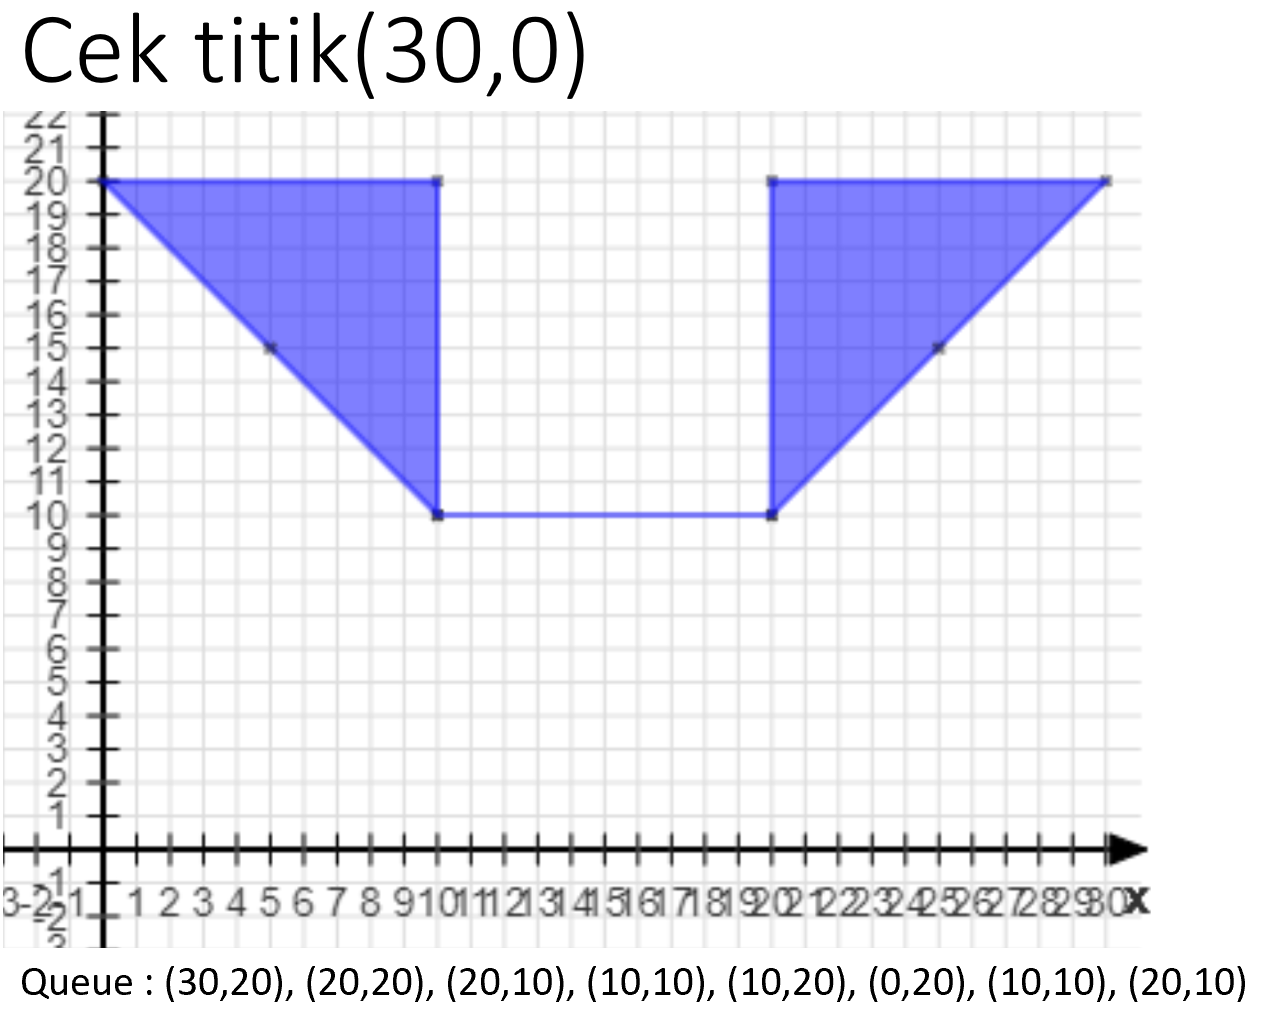
\includegraphics [width=\columnwidth]{bab5/img/iterasi-2}
	\caption {Ilustrasi Iterasi 2}
	\label {fig:iterasi-2}
\end{figure}

\par Pada awal iterasi ke-3, memeriksa titik $(30,20)$. Titik tersebut akan dibuang karena titik tersebut merupakan titik luar dan orientasi terhadap titik sebelumnya dan sesudahnya membentuk \textit{convex}. Sebelum membuang titik tersebut, program membuat segitiga dengan titik sebelumnya, titik tersebut dan titik sesudahnya. Kemudian program mencari semua titik yang berada di dalam segitiga tersebut. Selanjutnya program mencari \textit{convex hull} dari semua titik yang didapatkan dan disisipkan ke queue polygon luar untuk menggantikan titik yang dibuang. Kondisi setelah iterasi ke-3 dapat dilihat pada gambar \ref{fig:iterasi-3}.
\begin{figure}[!h]
	\Centering
	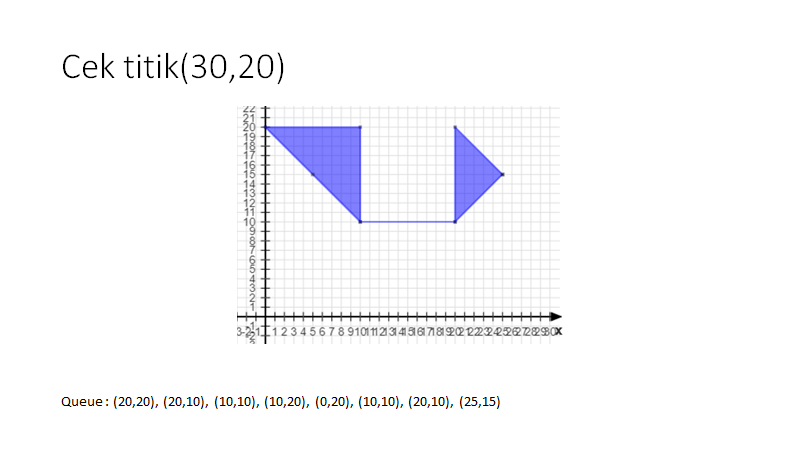
\includegraphics [width=\columnwidth]{bab5/img/iterasi-3}
	\caption {Ilustrasi Iterasi 3}
	\label {fig:iterasi-3}
\end{figure}

\par Pada awal iterasi ke-4, memeriksa titik $(20,20)$. Titik tersebut akan dibuang karena titik tersebut merupakan titik luar dan orientasi terhadap titik sebelumnya dan sesudahnya membentuk \textit{convex}. Sebelum membuang titik tersebut, program membuat segitiga dengan titik sebelumnya, titik tersebut dan titik sesudahnya. Kemudian program mencari semua titik yang berada di dalam segitiga tersebut. Selanjutnya program mencari \textit{convex hull} dari semua titik yang didapatkan dan disisipkan ke queue polygon luar untuk menggantikan titik yang dibuang. Kondisi setelah iterasi ke-4 dapat dilihat pada gambar \ref{fig:iterasi-4}.
\begin{figure}[!h]
	\Centering
	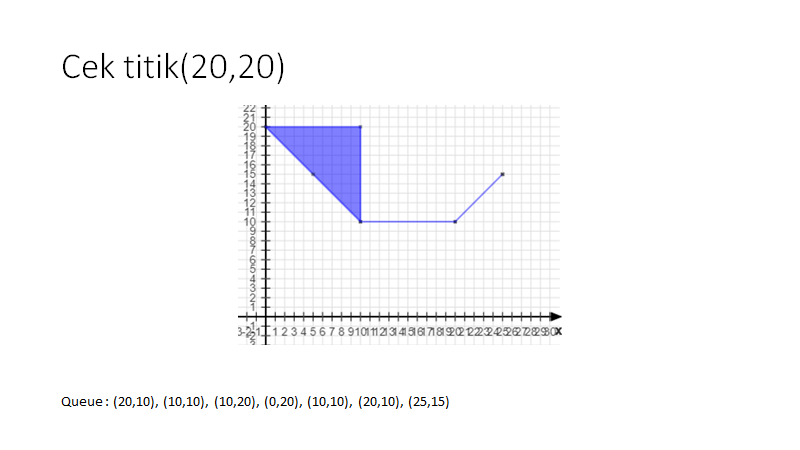
\includegraphics [width=\columnwidth]{bab5/img/iterasi-4}
	\caption {Ilustrasi Iterasi 4}
	\label {fig:iterasi-4}
\end{figure}

\par Pada awal iterasi ke-5, memeriksa titik $(20,10)$. Titik tersebut tidak akan dibuang karena titik tersebut merupakan titik luar tetapi orientasi terhadap titik sebelumnya dan sesudahnya membentuk \textit{concave}. Kondisi setelah iterasi ke-5 dapat dilihat pada gambar \ref{fig:iterasi-5}.
\begin{figure}[!h]
	\Centering
	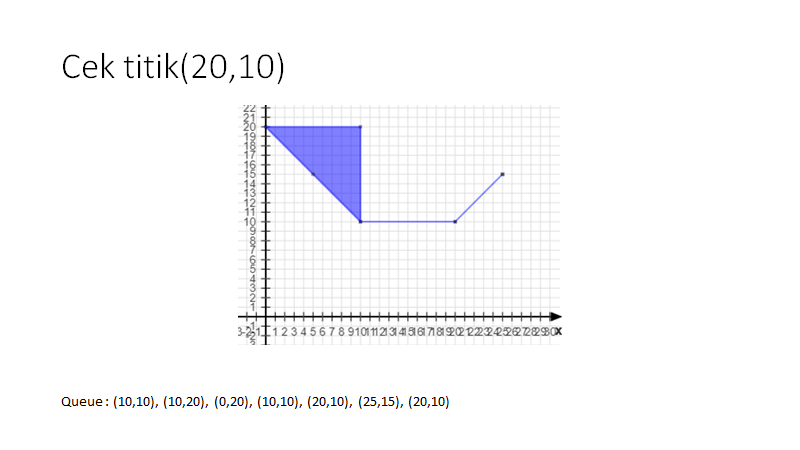
\includegraphics [width=\columnwidth]{bab5/img/iterasi-5}
	\caption {Ilustrasi Iterasi 5}
	\label {fig:iterasi-5}
\end{figure}

\par Pada awal iterasi ke-6, memeriksa titik $(10,10)$. Titik tersebut tidak akan dibuang karena titik tersebut merupakan titik luar tetapi orientasi terhadap titik sebelumnya dan sesudahnya membentuk \textit{concave}. Kondisi setelah iterasi ke-6 dapat dilihat pada gambar \ref{fig:iterasi-6}.
\begin{figure}[!h]
	\Centering
	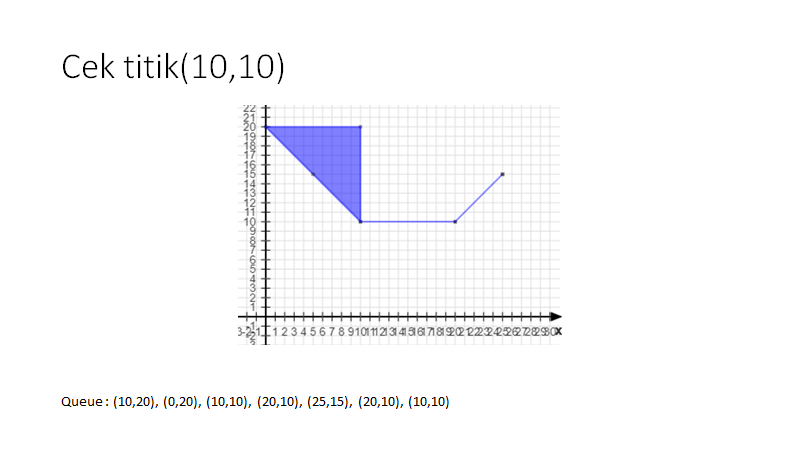
\includegraphics [width=\columnwidth]{bab5/img/iterasi-6}
	\caption {Ilustrasi Iterasi 6}
	\label {fig:iterasi-6}
\end{figure}

\par Pada awal iterasi ke-7, memeriksa titik $(10,20)$. Titik tersebut akan dibuang karena titik tersebut merupakan titik luar dan orientasi terhadap titik sebelumnya dan sesudahnya membentuk \textit{convex}. Sebelum membuang titik tersebut, program membuat segitiga dengan titik sebelumnya, titik tersebut dan titik sesudahnya. Kemudian program mencari semua titik yang berada di dalam segitiga tersebut. Selanjutnya program mencari \textit{convex hull} dari semua titik yang didapatkan dan disisipkan ke queue polygon luar untuk menggantikan titik yang dibuang. Kondisi setelah iterasi ke-7 dapat dilihat pada gambar \ref{fig:iterasi-7}.
\begin{figure}[!h]
	\Centering
	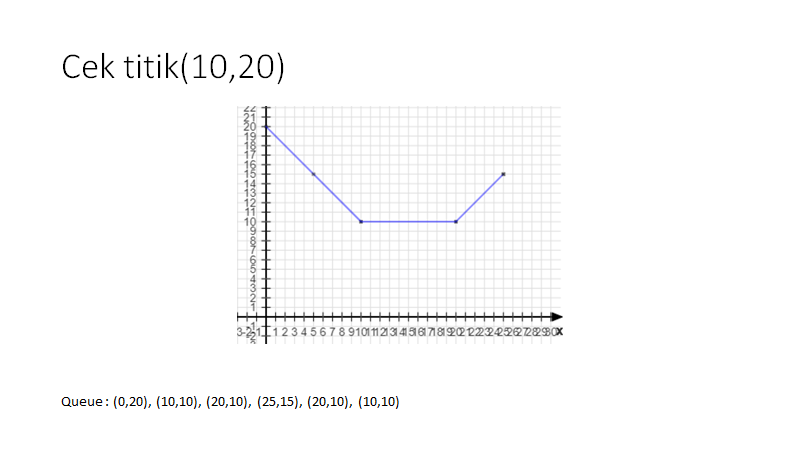
\includegraphics [width=\columnwidth]{bab5/img/iterasi-7}
	\caption {Ilustrasi Iterasi 7}
	\label {fig:iterasi-7}
\end{figure}

\par Pada awal iterasi ke-8, memeriksa titik $(0,20)$. Titik tersebut akan dibuang karena titik tersebut merupakan titik luar dan orientasi terhadap titik sebelumnya dan sesudahnya membentuk \textit{convex}. Sebelum membuang titik tersebut, program membuat segitiga dengan titik sebelumnya, titik tersebut dan titik sesudahnya. Kemudian program mencari semua titik yang berada di dalam segitiga tersebut. Selanjutnya program mencari \textit{convex hull} dari semua titik yang didapatkan dan disisipkan ke queue polygon luar untuk menggantikan titik yang dibuang. Kondisi setelah iterasi ke-8 dapat dilihat pada gambar \ref{fig:iterasi-8}.
\begin{figure}[!h]
	\Centering
	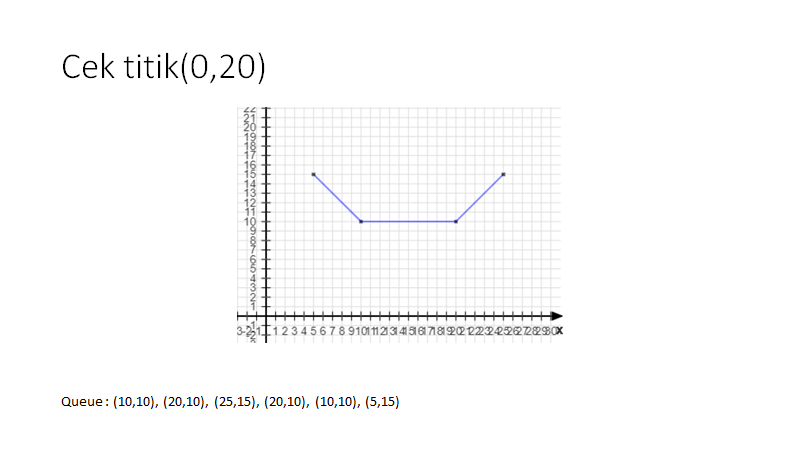
\includegraphics [width=\columnwidth]{bab5/img/iterasi-8}
	\caption {Ilustrasi Iterasi 8}
	\label {fig:iterasi-8}
\end{figure}

\section{Uji Coba Kinerja Luar}
Pada subbab ini akan ditampilkan hasil uji coba kinerja dari algoritma reduksi polygon. Pengujian dilakukan dengan cara mengirimkan kode program ke situs penilaian daring Sphere Online Judge. Detil mengenai hasil uji kinerja dapat dilihat pada Lampiran. Rata-rata hasil pengumpulan kode berkas dengan algoritma \textit{Melkman Convex Hull} adalah 0.08 detik dengan memori 4.6 MB. Hasil uji coba pada situs Sphere Online Judge dapat dilihat pada gambar \ref{fig:grafik-waktu-uji-coba-spoj} dan \ref{fig:grafik-memori-uji-coba-spoj}.
\begin{figure}[!h]
	\Centering
	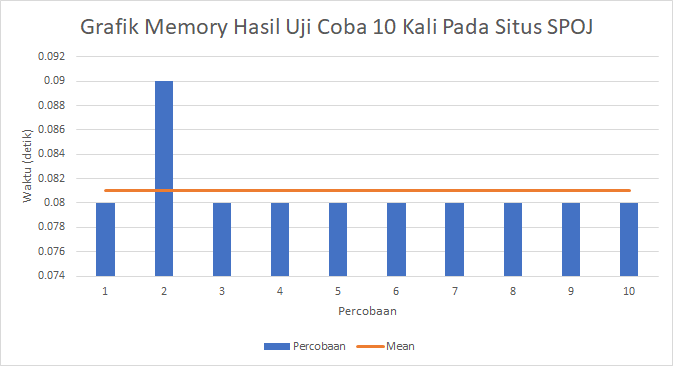
\includegraphics [width=\columnwidth]{bab5/img/grafik-waktu-uji-coba-spoj}
	\caption {Grafik Waktu Uji Coba 10 Kali pada Situs SPOJ}
	\label {fig:grafik-waktu-uji-coba-spoj}
\end{figure}
\begin{figure}[!h]
	\Centering
	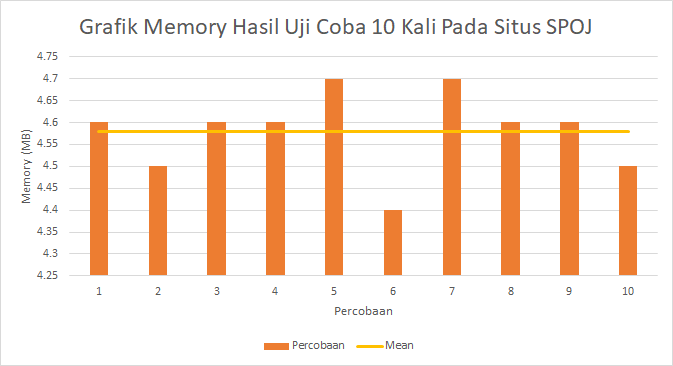
\includegraphics [width=\columnwidth]{bab5/img/grafik-memori-uji-coba-spoj}
	\caption {Grafik Memori Uji Coba 10 Kali pada Situs SPOJ}
	\label {fig:grafik-memori-uji-coba-spoj}
\end{figure}

 \cleardoublepage
	% 	\chapter{KESIMPULAN}
Pada bab ini dijelaskan mengenai kesimpulan dari hasil uji coba yang telah dilakukan serta saran-saran tentang pengembangan yang dapat dilakukan terhadap Tugas Akhir ini di masa yang akan datang.
\section{ Kesimpulan}
Berdasarkan penjabaran di bab-bab sebelumnya, dapat disimpulkan beberapa poin terkait penyelesaian permasalahan LL and Erbao.
\begin{enumerate}
\item Permasalahan LL and ErBao dapat diselesaikan dengan melakukan reduksi polygon luar terhadap titik di dalamnya.
\item Permasalahan LL and Erbao dapat diselesaikan dengan batasan pada soal dapat diselesaikan dengan reduksi polygon dengan waktu minimum 0.08 detik, waktu maksimum 0.08 detik, dan memori minimum 4.4 MB, memori maksimum 4.7 MB.
\item Algoritma \textit{Melkman convex hull} terbukti efektif untuk melakukan reduksi polygon untuk mencari \textit{relative convex polygon}.
\end{enumerate}
\section{ Saran}
Pada Tugas Akhir kali ini tentunya terdapat kekurangan serta nilai-nilai yang dapat penulis ambil. Berikut adalah saran-saran yang dapat diambil melalui Tugas Akhir ini:
\begin{enumerate}
 \item Untuk kedepannya, algoritma pada Tugas Akhir ini dapat menjadi bahan riset untuk mencari optimasi lebih lanjut.
 \item Metode reduksi polygon dengan menggunakan algoritma \textit{Melkman convex hull} yang dimodifikasi dapat digunakan untuk mencari \textit{relative convex hull} dengan polygon yang membatasi segmen garis ataupun polygon sederhana.
\end{enumerate} \cleardoublepage
	
	\backmatter
	 	\printbibliography
	% 	\chapter{LAMPIRAN A: Hasil Pengujian Untuk Kelompok N Tetap}

\newcounter{tablepart}
\setcounter{tablepart}{1}
\setcounter{table}{0}
\renewcommand{\thetable}{A.\arabic{table}}

\begin{table}[h!]
\Centering
\caption{Tabel hasil pengujian untuk kelompok N tetap (bg. \arabic{tablepart})}
\stepcounter{tablepart}
\begin{testtable}
1	&333	&99	&PASS	&333	&99	&PASS	\\
2	&178	&199	&PASS	&178	&199	&PASS	\\
3	&111	&406	&PASS	&111	&406	&PASS	\\
4	&684	&631	&PASS	&684	&631	&PASS	\\
5	&212	&33	&PASS	&212	&33	&PASS	\\
6	&256	&760	&PASS	&256	&760	&PASS	\\
7	&997	&392	&PASS	&997	&392	&PASS	\\
8	&397	&393	&PASS	&397	&393	&PASS	\\
9	&486	&323	&PASS	&486	&323	&PASS	\\
10	&477	&469	&PASS	&477	&469	&PASS	\\
11	&38	&479	&PASS	&38	&479	&PASS	\\
12	&132	&350	&PASS	&132	&350	&PASS	\\
13	&134	&781	&PASS	&134	&781	&PASS	\\
14	&638	&169	&PASS	&638	&169	&PASS	\\
15	&1013	&865	&PASS	&1013	&865	&PASS	\\
16	&517	&159	&PASS	&517	&159	&PASS	\\
17	&200	&502	&PASS	&200	&502	&PASS	\\
18	&157	&159	&PASS	&157	&159	&PASS	\\
19	&241	&272	&PASS	&241	&272	&PASS	\\
20	&111	&11	&PASS	&111	&11	&PASS	\\
21	&466	&285	&PASS	&466	&285	&PASS	\\
22	&142	&633	&PASS	&142	&633	&PASS	\\
23	&580	&394	&PASS	&580	&394	&PASS	\\
24	&344	&368	&PASS	&344	&368	&PASS	\\
25	&179	&149	&PASS	&179	&149	&PASS	\\
\end{testtable}
\end{table}
\begin{table}[h!]
\Centering
\caption{Tabel hasil pengujian untuk kelompok N tetap (bg. \arabic{tablepart})}
\stepcounter{tablepart}
\begin{testtable}
26	&476	&152	&PASS	&476	&152	&PASS	\\
27	&68	&140	&PASS	&68	&140	&PASS	\\
28	&372	&351	&PASS	&372	&351	&PASS	\\
29	&195	&371	&PASS	&195	&371	&PASS	\\
30	&535	&532	&PASS	&535	&532	&PASS	\\
31	&485	&437	&PASS	&485	&437	&PASS	\\
32	&122	&573	&PASS	&122	&573	&PASS	\\
33	&590	&508	&PASS	&590	&508	&PASS	\\
34	&58	&389	&PASS	&58	&389	&PASS	\\
35	&194	&189	&PASS	&194	&189	&PASS	\\
36	&69	&20	&PASS	&69	&20	&PASS	\\
37	&277	&423	&PASS	&277	&423	&PASS	\\
38	&463	&8	&PASS	&463	&8	&PASS	\\
39	&126	&249	&PASS	&126	&249	&PASS	\\
40	&253	&360	&PASS	&253	&360	&PASS	\\
41	&121	&249	&PASS	&121	&249	&PASS	\\
42	&203	&283	&PASS	&203	&283	&PASS	\\
43	&126	&356	&PASS	&126	&356	&PASS	\\
44	&470	&385	&PASS	&470	&385	&PASS	\\
45	&36	&568	&PASS	&36	&568	&PASS	\\
46	&433	&494	&PASS	&433	&494	&PASS	\\
47	&107	&546	&PASS	&107	&546	&PASS	\\
48	&395	&509	&PASS	&395	&509	&PASS	\\
49	&37	&224	&PASS	&37	&224	&PASS	\\
50	&125	&75	&PASS	&125	&75	&PASS	\\
\end{testtable}
\end{table}
\begin{table}[h!]
\Centering
\caption{Tabel hasil pengujian untuk kelompok N tetap (bg. \arabic{tablepart})}
\stepcounter{tablepart}
\begin{testtable}
51	&321	&118	&PASS	&321	&118	&PASS	\\
52	&128	&214	&PASS	&128	&214	&PASS	\\
53	&32	&542	&PASS	&32	&542	&PASS	\\
54	&165	&305	&PASS	&165	&305	&PASS	\\
55	&224	&228	&PASS	&224	&228	&PASS	\\
56	&132	&51	&PASS	&132	&51	&PASS	\\
57	&284	&14	&PASS	&284	&14	&PASS	\\
58	&250	&352	&PASS	&250	&352	&PASS	\\
59	&165	&363	&PASS	&165	&363	&PASS	\\
60	&488	&464	&PASS	&488	&464	&PASS	\\
61	&56	&312	&PASS	&56	&312	&PASS	\\
62	&469	&98	&PASS	&469	&98	&PASS	\\
63	&415	&359	&PASS	&415	&359	&PASS	\\
64	&546	&173	&PASS	&546	&173	&PASS	\\
65	&480	&534	&PASS	&480	&534	&PASS	\\
66	&415	&257	&PASS	&415	&257	&PASS	\\
67	&144	&267	&PASS	&144	&267	&PASS	\\
68	&500	&434	&PASS	&500	&434	&PASS	\\
69	&336	&235	&PASS	&336	&235	&PASS	\\
70	&281	&68	&PASS	&281	&68	&PASS	\\
71	&293	&88	&PASS	&293	&88	&PASS	\\
72	&500	&539	&PASS	&500	&539	&PASS	\\
73	&264	&510	&PASS	&264	&510	&PASS	\\
74	&534	&253	&PASS	&534	&253	&PASS	\\
75	&457	&501	&PASS	&457	&501	&PASS	\\
\end{testtable}
\end{table}
\begin{table}[h!]
\Centering
\caption{Tabel hasil pengujian untuk kelompok N tetap (bg. \arabic{tablepart})}
\stepcounter{tablepart}
\begin{testtable}
76	&465	&253	&PASS	&465	&253	&PASS	\\
77	&226	&365	&PASS	&226	&365	&PASS	\\
78	&467	&62	&PASS	&467	&62	&PASS	\\
79	&421	&276	&PASS	&421	&276	&PASS	\\
80	&284	&127	&PASS	&284	&127	&PASS	\\
81	&340	&419	&PASS	&340	&419	&PASS	\\
82	&256	&216	&PASS	&256	&216	&PASS	\\
83	&325	&89	&PASS	&325	&89	&PASS	\\
84	&446	&243	&PASS	&446	&243	&PASS	\\
85	&332	&427	&PASS	&332	&427	&PASS	\\
86	&355	&290	&PASS	&355	&290	&PASS	\\
87	&170	&119	&PASS	&170	&119	&PASS	\\
88	&521	&29	&PASS	&521	&29	&PASS	\\
89	&299	&484	&PASS	&299	&484	&PASS	\\
90	&37	&274	&PASS	&37	&274	&PASS	\\
91	&485	&504	&PASS	&485	&504	&PASS	\\
92	&204	&392	&PASS	&204	&392	&PASS	\\
93	&476	&466	&PASS	&476	&466	&PASS	\\
94	&291	&546	&PASS	&291	&546	&PASS	\\
95	&302	&318	&PASS	&302	&318	&PASS	\\
96	&357	&190	&PASS	&357	&190	&PASS	\\
97	&180	&385	&PASS	&180	&385	&PASS	\\
98	&102	&301	&PASS	&102	&301	&PASS	\\
99	&429	&124	&PASS	&429	&124	&PASS	\\
100	&430	&402	&PASS	&430	&402	&PASS	\\
\end{testtable}
\end{table}
\begin{table}[h!]
\Centering
\caption{Tabel hasil pengujian untuk kelompok N tetap (bg. \arabic{tablepart})}
\stepcounter{tablepart}
\begin{testtable}
101	&156	&537	&PASS	&156	&537	&PASS	\\
102	&5	&239	&PASS	&5	&239	&PASS	\\
103	&260	&379	&PASS	&260	&379	&PASS	\\
104	&38	&459	&PASS	&38	&459	&PASS	\\
105	&33	&447	&PASS	&33	&447	&PASS	\\
106	&473	&105	&PASS	&473	&105	&PASS	\\
107	&198	&327	&PASS	&198	&327	&PASS	\\
108	&264	&123	&PASS	&264	&123	&PASS	\\
109	&22	&247	&PASS	&22	&247	&PASS	\\
110	&364	&168	&PASS	&364	&168	&PASS	\\
111	&319	&494	&PASS	&319	&494	&PASS	\\
112	&131	&30	&PASS	&131	&30	&PASS	\\
113	&281	&45	&PASS	&281	&45	&PASS	\\
114	&34	&297	&PASS	&34	&297	&PASS	\\
115	&102	&15	&PASS	&102	&15	&PASS	\\
116	&86	&151	&PASS	&86	&151	&PASS	\\
117	&289	&463	&PASS	&289	&463	&PASS	\\
118	&543	&473	&PASS	&543	&473	&PASS	\\
119	&225	&531	&PASS	&225	&531	&PASS	\\
120	&240	&174	&PASS	&240	&174	&PASS	\\
121	&140	&99	&PASS	&140	&99	&PASS	\\
122	&57	&323	&PASS	&57	&323	&PASS	\\
123	&65	&46	&PASS	&65	&46	&PASS	\\
124	&528	&302	&PASS	&528	&302	&PASS	\\
125	&77	&356	&PASS	&77	&356	&PASS	\\
\end{testtable}
\end{table}
\begin{table}[h!]
\Centering
\caption{Tabel hasil pengujian untuk kelompok N tetap (bg. \arabic{tablepart})}
\stepcounter{tablepart}
\begin{testtable}
126	&158	&241	&PASS	&158	&241	&PASS	\\
127	&76	&231	&PASS	&76	&231	&PASS	\\
128	&179	&181	&PASS	&179	&181	&PASS	\\
129	&522	&114	&PASS	&522	&114	&PASS	\\
130	&247	&272	&PASS	&247	&272	&PASS	\\
131	&428	&189	&PASS	&428	&189	&PASS	\\
132	&381	&52	&PASS	&381	&52	&PASS	\\
133	&121	&144	&PASS	&121	&144	&PASS	\\
134	&267	&167	&PASS	&267	&167	&PASS	\\
135	&428	&114	&PASS	&428	&114	&PASS	\\
136	&228	&281	&PASS	&228	&281	&PASS	\\
137	&351	&126	&PASS	&351	&126	&PASS	\\
138	&151	&535	&PASS	&151	&535	&PASS	\\
139	&523	&432	&PASS	&523	&432	&PASS	\\
140	&262	&538	&PASS	&262	&538	&PASS	\\
141	&46	&501	&PASS	&46	&501	&PASS	\\
142	&448	&489	&PASS	&448	&489	&PASS	\\
143	&18	&186	&PASS	&18	&186	&PASS	\\
144	&416	&118	&PASS	&416	&118	&PASS	\\
145	&412	&198	&PASS	&412	&198	&PASS	\\
146	&382	&397	&PASS	&382	&397	&PASS	\\
147	&107	&429	&PASS	&107	&429	&PASS	\\
148	&242	&215	&PASS	&242	&215	&PASS	\\
149	&238	&126	&PASS	&238	&126	&PASS	\\
150	&299	&349	&PASS	&299	&349	&PASS	\\
\end{testtable}
\end{table}
\begin{table}[h!]
\Centering
\caption{Tabel hasil pengujian untuk kelompok N tetap (bg. \arabic{tablepart})}
\stepcounter{tablepart}
\begin{testtable}
151	&221	&345	&PASS	&221	&345	&PASS	\\
152	&306	&26	&PASS	&306	&26	&PASS	\\
153	&510	&374	&PASS	&510	&374	&PASS	\\
154	&266	&163	&PASS	&266	&163	&PASS	\\
155	&376	&229	&PASS	&376	&229	&PASS	\\
156	&423	&401	&PASS	&423	&401	&PASS	\\
157	&11	&221	&PASS	&11	&221	&PASS	\\
158	&18	&22	&PASS	&18	&22	&PASS	\\
159	&353	&334	&PASS	&353	&334	&PASS	\\
160	&69	&46	&PASS	&69	&46	&PASS	\\
161	&373	&418	&PASS	&373	&418	&PASS	\\
162	&105	&478	&PASS	&105	&478	&PASS	\\
163	&382	&21	&PASS	&382	&21	&PASS	\\
164	&119	&529	&PASS	&119	&529	&PASS	\\
165	&348	&448	&PASS	&348	&448	&PASS	\\
166	&296	&84	&PASS	&296	&84	&PASS	\\
167	&493	&72	&PASS	&493	&72	&PASS	\\
168	&74	&287	&PASS	&74	&287	&PASS	\\
169	&349	&423	&PASS	&349	&423	&PASS	\\
170	&399	&427	&PASS	&399	&427	&PASS	\\
171	&538	&187	&PASS	&538	&187	&PASS	\\
172	&110	&349	&PASS	&110	&349	&PASS	\\
173	&359	&105	&PASS	&359	&105	&PASS	\\
174	&176	&187	&PASS	&176	&187	&PASS	\\
175	&335	&208	&PASS	&335	&208	&PASS	\\
\end{testtable}
\end{table}
\begin{table}[h!]
\Centering
\caption{Tabel hasil pengujian untuk kelompok N tetap (bg. \arabic{tablepart})}
\stepcounter{tablepart}
\begin{testtable}
176	&212	&469	&PASS	&212	&469	&PASS	\\
177	&439	&516	&PASS	&439	&516	&PASS	\\
178	&237	&394	&PASS	&237	&394	&PASS	\\
179	&239	&303	&PASS	&239	&303	&PASS	\\
180	&279	&323	&PASS	&279	&323	&PASS	\\
181	&327	&135	&PASS	&327	&135	&PASS	\\
182	&282	&163	&PASS	&282	&163	&PASS	\\
183	&503	&306	&PASS	&503	&306	&PASS	\\
184	&387	&362	&PASS	&387	&362	&PASS	\\
185	&543	&284	&PASS	&543	&284	&PASS	\\
186	&247	&182	&PASS	&247	&182	&PASS	\\
187	&141	&342	&PASS	&141	&342	&PASS	\\
188	&231	&38	&PASS	&231	&38	&PASS	\\
189	&244	&91	&PASS	&244	&91	&PASS	\\
190	&80	&422	&PASS	&80	&422	&PASS	\\
191	&189	&71	&PASS	&189	&71	&PASS	\\
192	&426	&427	&PASS	&426	&427	&PASS	\\
193	&357	&172	&PASS	&357	&172	&PASS	\\
194	&526	&43	&PASS	&526	&43	&PASS	\\
195	&492	&483	&PASS	&492	&483	&PASS	\\
196	&137	&23	&PASS	&137	&23	&PASS	\\
197	&528	&91	&PASS	&528	&91	&PASS	\\
198	&216	&492	&PASS	&216	&492	&PASS	\\
199	&360	&147	&PASS	&360	&147	&PASS	\\
200	&309	&96	&PASS	&309	&96	&PASS	\\
\end{testtable}
\end{table}
\begin{table}[h!]
\Centering
\caption{Tabel hasil pengujian untuk kelompok N tetap (bg. \arabic{tablepart})}
\stepcounter{tablepart}
\begin{testtable}
201	&526	&311	&PASS	&526	&311	&PASS	\\
202	&431	&287	&PASS	&431	&287	&PASS	\\
203	&307	&323	&PASS	&307	&323	&PASS	\\
204	&390	&90	&PASS	&390	&90	&PASS	\\
205	&333	&186	&PASS	&333	&186	&PASS	\\
206	&207	&365	&PASS	&207	&365	&PASS	\\
207	&71	&437	&PASS	&71	&437	&PASS	\\
208	&243	&246	&PASS	&243	&246	&PASS	\\
209	&6	&189	&PASS	&6	&189	&PASS	\\
210	&470	&314	&PASS	&470	&314	&PASS	\\
211	&53	&417	&PASS	&53	&417	&PASS	\\
212	&162	&535	&PASS	&162	&535	&PASS	\\
213	&529	&266	&PASS	&529	&266	&PASS	\\
214	&426	&484	&PASS	&426	&484	&PASS	\\
215	&490	&69	&PASS	&490	&69	&PASS	\\
216	&502	&251	&PASS	&502	&251	&PASS	\\
217	&129	&16	&PASS	&129	&16	&PASS	\\
218	&121	&519	&PASS	&121	&519	&PASS	\\
219	&154	&173	&PASS	&154	&173	&PASS	\\
220	&74	&452	&PASS	&74	&452	&PASS	\\
221	&395	&464	&PASS	&395	&464	&PASS	\\
222	&450	&56	&PASS	&450	&56	&PASS	\\
223	&52	&207	&PASS	&52	&207	&PASS	\\
224	&168	&153	&PASS	&168	&153	&PASS	\\
225	&363	&244	&PASS	&363	&244	&PASS	\\
\end{testtable}
\end{table}
\begin{table}[h!]
\Centering
\caption{Tabel hasil pengujian untuk kelompok N tetap (bg. \arabic{tablepart})}
\stepcounter{tablepart}
\begin{testtable}
226	&441	&454	&PASS	&441	&454	&PASS	\\
227	&163	&376	&PASS	&163	&376	&PASS	\\
228	&237	&109	&PASS	&237	&109	&PASS	\\
229	&493	&84	&PASS	&493	&84	&PASS	\\
230	&118	&149	&PASS	&118	&149	&PASS	\\
231	&252	&8	&PASS	&252	&8	&PASS	\\
232	&346	&340	&PASS	&346	&340	&PASS	\\
233	&304	&389	&PASS	&304	&389	&PASS	\\
234	&320	&266	&PASS	&320	&266	&PASS	\\
235	&334	&432	&PASS	&334	&432	&PASS	\\
236	&404	&135	&PASS	&404	&135	&PASS	\\
237	&29	&217	&PASS	&29	&217	&PASS	\\
238	&346	&64	&PASS	&346	&64	&PASS	\\
239	&523	&431	&PASS	&523	&431	&PASS	\\
240	&192	&140	&PASS	&192	&140	&PASS	\\
241	&90	&256	&PASS	&90	&256	&PASS	\\
242	&139	&442	&PASS	&139	&442	&PASS	\\
243	&219	&443	&PASS	&219	&443	&PASS	\\
244	&522	&148	&PASS	&522	&148	&PASS	\\
245	&341	&524	&PASS	&341	&524	&PASS	\\
246	&296	&249	&PASS	&296	&249	&PASS	\\
247	&472	&271	&PASS	&472	&271	&PASS	\\
248	&417	&419	&PASS	&417	&419	&PASS	\\
249	&179	&473	&PASS	&179	&473	&PASS	\\
250	&178	&129	&PASS	&178	&129	&PASS	\\
\end{testtable}
\end{table}
\begin{table}[h!]
\Centering
\caption{Tabel hasil pengujian untuk kelompok N tetap (bg. \arabic{tablepart})}
\stepcounter{tablepart}
\begin{testtable}
251	&327	&129	&PASS	&327	&129	&PASS	\\
252	&243	&361	&PASS	&243	&361	&PASS	\\
253	&543	&204	&PASS	&543	&204	&PASS	\\
254	&207	&215	&PASS	&207	&215	&PASS	\\
255	&61	&24	&PASS	&61	&24	&PASS	\\
256	&503	&20	&PASS	&503	&20	&PASS	\\
257	&356	&543	&PASS	&356	&543	&PASS	\\
258	&461	&195	&PASS	&461	&195	&PASS	\\
259	&542	&497	&PASS	&542	&497	&PASS	\\
260	&531	&148	&PASS	&531	&148	&PASS	\\
261	&515	&244	&PASS	&515	&244	&PASS	\\
262	&191	&380	&PASS	&191	&380	&PASS	\\
263	&124	&117	&PASS	&124	&117	&PASS	\\
264	&431	&238	&PASS	&431	&238	&PASS	\\
265	&508	&54	&PASS	&508	&54	&PASS	\\
266	&114	&335	&PASS	&114	&335	&PASS	\\
267	&210	&387	&PASS	&210	&387	&PASS	\\
268	&30	&487	&PASS	&30	&487	&PASS	\\
269	&13	&61	&PASS	&13	&61	&PASS	\\
270	&323	&177	&PASS	&323	&177	&PASS	\\
271	&229	&527	&PASS	&229	&527	&PASS	\\
272	&67	&188	&PASS	&67	&188	&PASS	\\
273	&511	&178	&PASS	&511	&178	&PASS	\\
274	&360	&292	&PASS	&360	&292	&PASS	\\
275	&424	&186	&PASS	&424	&186	&PASS	\\
\end{testtable}
\end{table}
\begin{table}[h!]
\Centering
\caption{Tabel hasil pengujian untuk kelompok N tetap (bg. \arabic{tablepart})}
\stepcounter{tablepart}
\begin{testtable}
276	&198	&291	&PASS	&198	&291	&PASS	\\
277	&332	&121	&PASS	&332	&121	&PASS	\\
278	&249	&76	&PASS	&249	&76	&PASS	\\
279	&525	&61	&PASS	&525	&61	&PASS	\\
280	&230	&447	&PASS	&230	&447	&PASS	\\
281	&119	&498	&PASS	&119	&498	&PASS	\\
282	&479	&251	&PASS	&479	&251	&PASS	\\
283	&532	&220	&PASS	&532	&220	&PASS	\\
284	&349	&164	&PASS	&349	&164	&PASS	\\
285	&492	&173	&PASS	&492	&173	&PASS	\\
286	&207	&79	&PASS	&207	&79	&PASS	\\
287	&514	&315	&PASS	&514	&315	&PASS	\\
288	&351	&540	&PASS	&351	&540	&PASS	\\
289	&344	&249	&PASS	&344	&249	&PASS	\\
290	&309	&264	&PASS	&309	&264	&PASS	\\
291	&246	&427	&PASS	&246	&427	&PASS	\\
292	&280	&30	&PASS	&280	&30	&PASS	\\
293	&75	&477	&PASS	&75	&477	&PASS	\\
294	&436	&372	&PASS	&436	&372	&PASS	\\
295	&300	&304	&PASS	&300	&304	&PASS	\\
296	&501	&102	&PASS	&501	&102	&PASS	\\
297	&273	&275	&PASS	&273	&275	&PASS	\\
298	&269	&103	&PASS	&269	&103	&PASS	\\
299	&514	&65	&PASS	&514	&65	&PASS	\\
300	&419	&195	&PASS	&419	&195	&PASS	\\
\end{testtable}
\end{table}
\begin{table}[h!]
\Centering
\caption{Tabel hasil pengujian untuk kelompok N tetap (bg. \arabic{tablepart})}
\stepcounter{tablepart}
\begin{testtable}
301	&541	&478	&PASS	&541	&478	&PASS	\\
302	&112	&237	&PASS	&112	&237	&PASS	\\
303	&38	&59	&PASS	&38	&59	&PASS	\\
304	&518	&101	&PASS	&518	&101	&PASS	\\
305	&48	&421	&PASS	&48	&421	&PASS	\\
306	&97	&339	&PASS	&97	&339	&PASS	\\
307	&117	&275	&PASS	&117	&275	&PASS	\\
308	&535	&220	&PASS	&535	&220	&PASS	\\
309	&266	&136	&PASS	&266	&136	&PASS	\\
310	&159	&391	&PASS	&159	&391	&PASS	\\
311	&391	&144	&PASS	&391	&144	&PASS	\\
312	&55	&458	&PASS	&55	&458	&PASS	\\
313	&209	&218	&PASS	&209	&218	&PASS	\\
314	&482	&50	&PASS	&482	&50	&PASS	\\
315	&544	&237	&PASS	&544	&237	&PASS	\\
316	&39	&92	&PASS	&39	&92	&PASS	\\
317	&346	&472	&PASS	&346	&472	&PASS	\\
318	&268	&178	&PASS	&268	&178	&PASS	\\
319	&251	&293	&PASS	&251	&293	&PASS	\\
320	&424	&311	&PASS	&424	&311	&PASS	\\
321	&304	&468	&PASS	&304	&468	&PASS	\\
322	&62	&539	&PASS	&62	&539	&PASS	\\
323	&231	&546	&PASS	&231	&546	&PASS	\\
324	&93	&227	&PASS	&93	&227	&PASS	\\
325	&176	&193	&PASS	&176	&193	&PASS	\\
\end{testtable}
\end{table}
\begin{table}[h!]
\Centering
\caption{Tabel hasil pengujian untuk kelompok N tetap (bg. \arabic{tablepart})}
\stepcounter{tablepart}
\begin{testtable}
326	&137	&291	&PASS	&137	&291	&PASS	\\
327	&479	&51	&PASS	&479	&51	&PASS	\\
328	&446	&86	&PASS	&446	&86	&PASS	\\
329	&315	&100	&PASS	&315	&100	&PASS	\\
330	&100	&536	&PASS	&100	&536	&PASS	\\
331	&88	&150	&PASS	&88	&150	&PASS	\\
332	&438	&346	&PASS	&438	&346	&PASS	\\
333	&505	&13	&PASS	&505	&13	&PASS	\\
334	&190	&189	&PASS	&190	&189	&PASS	\\
335	&278	&43	&PASS	&278	&43	&PASS	\\
336	&175	&76	&PASS	&175	&76	&PASS	\\
337	&381	&537	&PASS	&381	&537	&PASS	\\
338	&292	&216	&PASS	&292	&216	&PASS	\\
339	&401	&428	&PASS	&401	&428	&PASS	\\
340	&407	&1	&PASS	&407	&1	&PASS	\\
341	&433	&493	&PASS	&433	&493	&PASS	\\
342	&476	&56	&PASS	&476	&56	&PASS	\\
343	&481	&406	&PASS	&481	&406	&PASS	\\
344	&44	&36	&PASS	&44	&36	&PASS	\\
345	&430	&224	&PASS	&430	&224	&PASS	\\
346	&17	&483	&PASS	&17	&483	&PASS	\\
347	&304	&469	&PASS	&304	&469	&PASS	\\
348	&437	&3	&PASS	&437	&3	&PASS	\\
349	&256	&170	&PASS	&256	&170	&PASS	\\
350	&283	&145	&PASS	&283	&145	&PASS	\\
\end{testtable}
\end{table}
\begin{table}[h!]
\Centering
\caption{Tabel hasil pengujian untuk kelompok N tetap (bg. \arabic{tablepart})}
\stepcounter{tablepart}
\begin{testtable}
351	&499	&143	&PASS	&499	&143	&PASS	\\
352	&90	&71	&PASS	&90	&71	&PASS	\\
353	&46	&118	&PASS	&46	&118	&PASS	\\
354	&23	&143	&PASS	&23	&143	&PASS	\\
355	&268	&531	&PASS	&268	&531	&PASS	\\
356	&534	&310	&PASS	&534	&310	&PASS	\\
357	&443	&244	&PASS	&443	&244	&PASS	\\
358	&20	&55	&PASS	&20	&55	&PASS	\\
359	&477	&333	&PASS	&477	&333	&PASS	\\
360	&151	&355	&PASS	&151	&355	&PASS	\\
361	&256	&59	&PASS	&256	&59	&PASS	\\
362	&241	&235	&PASS	&241	&235	&PASS	\\
363	&268	&70	&PASS	&268	&70	&PASS	\\
364	&536	&50	&PASS	&536	&50	&PASS	\\
365	&430	&208	&PASS	&430	&208	&PASS	\\
366	&332	&303	&PASS	&332	&303	&PASS	\\
367	&204	&42	&PASS	&204	&42	&PASS	\\
368	&537	&278	&PASS	&537	&278	&PASS	\\
369	&233	&399	&PASS	&233	&399	&PASS	\\
370	&178	&377	&PASS	&178	&377	&PASS	\\
371	&196	&297	&PASS	&196	&297	&PASS	\\
372	&148	&237	&PASS	&148	&237	&PASS	\\
373	&421	&450	&PASS	&421	&450	&PASS	\\
374	&472	&449	&PASS	&472	&449	&PASS	\\
375	&286	&140	&PASS	&286	&140	&PASS	\\
\end{testtable}
\end{table}
\begin{table}[h!]
\Centering
\caption{Tabel hasil pengujian untuk kelompok N tetap (bg. \arabic{tablepart})}
\stepcounter{tablepart}
\begin{testtable}
376	&237	&138	&PASS	&237	&138	&PASS	\\
377	&133	&397	&PASS	&133	&397	&PASS	\\
378	&37	&405	&PASS	&37	&405	&PASS	\\
379	&209	&176	&PASS	&209	&176	&PASS	\\
380	&348	&123	&PASS	&348	&123	&PASS	\\
381	&309	&374	&PASS	&309	&374	&PASS	\\
382	&314	&444	&PASS	&314	&444	&PASS	\\
383	&492	&226	&PASS	&492	&226	&PASS	\\
384	&505	&297	&PASS	&505	&297	&PASS	\\
385	&149	&153	&PASS	&149	&153	&PASS	\\
386	&211	&480	&PASS	&211	&480	&PASS	\\
387	&446	&481	&PASS	&446	&481	&PASS	\\
388	&133	&292	&PASS	&133	&292	&PASS	\\
389	&349	&67	&PASS	&349	&67	&PASS	\\
390	&234	&345	&PASS	&234	&345	&PASS	\\
391	&183	&376	&PASS	&183	&376	&PASS	\\
392	&527	&496	&PASS	&527	&496	&PASS	\\
393	&244	&213	&PASS	&244	&213	&PASS	\\
394	&435	&395	&PASS	&435	&395	&PASS	\\
395	&197	&218	&PASS	&197	&218	&PASS	\\
396	&398	&412	&PASS	&398	&412	&PASS	\\
397	&97	&85	&PASS	&97	&85	&PASS	\\
398	&470	&494	&PASS	&470	&494	&PASS	\\
399	&77	&23	&PASS	&77	&23	&PASS	\\
400	&338	&468	&PASS	&338	&468	&PASS	\\
\end{testtable}
\end{table}
\begin{table}[h!]
\Centering
\caption{Tabel hasil pengujian untuk kelompok N tetap (bg. \arabic{tablepart})}
\stepcounter{tablepart}
\begin{testtable}
401	&478	&34	&PASS	&478	&34	&PASS	\\
402	&412	&86	&PASS	&412	&86	&PASS	\\
403	&163	&202	&PASS	&163	&202	&PASS	\\
404	&469	&9	&PASS	&469	&9	&PASS	\\
405	&301	&126	&PASS	&301	&126	&PASS	\\
406	&33	&408	&PASS	&33	&408	&PASS	\\
407	&70	&35	&PASS	&70	&35	&PASS	\\
408	&176	&363	&PASS	&176	&363	&PASS	\\
409	&312	&496	&PASS	&312	&496	&PASS	\\
410	&249	&215	&PASS	&249	&215	&PASS	\\
411	&173	&172	&PASS	&173	&172	&PASS	\\
412	&204	&5	&PASS	&204	&5	&PASS	\\
413	&165	&358	&PASS	&165	&358	&PASS	\\
414	&180	&192	&PASS	&180	&192	&PASS	\\
415	&495	&481	&PASS	&495	&481	&PASS	\\
416	&38	&357	&PASS	&38	&357	&PASS	\\
417	&250	&525	&PASS	&250	&525	&PASS	\\
418	&237	&358	&PASS	&237	&358	&PASS	\\
419	&257	&286	&PASS	&257	&286	&PASS	\\
420	&98	&196	&PASS	&98	&196	&PASS	\\
421	&244	&267	&PASS	&244	&267	&PASS	\\
422	&458	&482	&PASS	&458	&482	&PASS	\\
423	&348	&6	&PASS	&348	&6	&PASS	\\
424	&334	&182	&PASS	&334	&182	&PASS	\\
425	&265	&262	&PASS	&265	&262	&PASS	\\
\end{testtable}
\end{table}
\begin{table}[h!]
\Centering
\caption{Tabel hasil pengujian untuk kelompok N tetap (bg. \arabic{tablepart})}
\stepcounter{tablepart}
\begin{testtable}
426	&313	&197	&PASS	&313	&197	&PASS	\\
427	&516	&243	&PASS	&516	&243	&PASS	\\
428	&54	&137	&PASS	&54	&137	&PASS	\\
429	&253	&76	&PASS	&253	&76	&PASS	\\
430	&492	&531	&PASS	&492	&531	&PASS	\\
431	&235	&379	&PASS	&235	&379	&PASS	\\
432	&1	&113	&PASS	&1	&113	&PASS	\\
433	&353	&31	&PASS	&353	&31	&PASS	\\
434	&73	&537	&PASS	&73	&537	&PASS	\\
435	&242	&135	&PASS	&242	&135	&PASS	\\
436	&131	&332	&PASS	&131	&332	&PASS	\\
437	&190	&340	&PASS	&190	&340	&PASS	\\
438	&155	&238	&PASS	&155	&238	&PASS	\\
439	&243	&277	&PASS	&243	&277	&PASS	\\
440	&11	&224	&PASS	&11	&224	&PASS	\\
441	&143	&100	&PASS	&143	&100	&PASS	\\
442	&414	&541	&PASS	&414	&541	&PASS	\\
443	&421	&177	&PASS	&421	&177	&PASS	\\
444	&376	&534	&PASS	&376	&534	&PASS	\\
445	&35	&393	&PASS	&35	&393	&PASS	\\
446	&148	&331	&PASS	&148	&331	&PASS	\\
447	&273	&48	&PASS	&273	&48	&PASS	\\
448	&194	&433	&PASS	&194	&433	&PASS	\\
449	&155	&465	&PASS	&155	&465	&PASS	\\
450	&82	&311	&PASS	&82	&311	&PASS	\\
\end{testtable}
\end{table}
\begin{table}[h!]
\Centering
\caption{Tabel hasil pengujian untuk kelompok N tetap (bg. \arabic{tablepart})}
\stepcounter{tablepart}
\begin{testtable}
451	&186	&505	&PASS	&186	&505	&PASS	\\
452	&35	&394	&PASS	&35	&394	&PASS	\\
453	&75	&3	&PASS	&75	&3	&PASS	\\
454	&308	&150	&PASS	&308	&150	&PASS	\\
455	&382	&413	&PASS	&382	&413	&PASS	\\
456	&372	&287	&PASS	&372	&287	&PASS	\\
457	&419	&110	&PASS	&419	&110	&PASS	\\
458	&469	&48	&PASS	&469	&48	&PASS	\\
459	&538	&49	&PASS	&538	&49	&PASS	\\
460	&224	&107	&PASS	&224	&107	&PASS	\\
461	&104	&277	&PASS	&104	&277	&PASS	\\
462	&513	&198	&PASS	&513	&198	&PASS	\\
463	&378	&294	&PASS	&378	&294	&PASS	\\
464	&257	&156	&PASS	&257	&156	&PASS	\\
465	&222	&363	&PASS	&222	&363	&PASS	\\
466	&109	&471	&PASS	&109	&471	&PASS	\\
467	&51	&511	&PASS	&51	&511	&PASS	\\
468	&478	&228	&PASS	&478	&228	&PASS	\\
469	&248	&469	&PASS	&248	&469	&PASS	\\
470	&6	&314	&PASS	&6	&314	&PASS	\\
471	&198	&369	&PASS	&198	&369	&PASS	\\
472	&240	&108	&PASS	&240	&108	&PASS	\\
473	&228	&68	&PASS	&228	&68	&PASS	\\
474	&149	&394	&PASS	&149	&394	&PASS	\\
475	&25	&378	&PASS	&25	&378	&PASS	\\
\end{testtable}
\end{table}
	% 	\chapter{LAMPIRAN B: Hasil Pengujian Untuk Kelompok L Tetap}

\setcounter{tablepart}{1}
\setcounter{table}{0}
\renewcommand{\thetable}{B.\arabic{table}}

\begin{table}[h!]
\Centering
\caption{Tabel hasil pengujian untuk kelompok N tetap (bg. \arabic{tablepart})}
\stepcounter{tablepart}
\begin{testtable}
1	&109	&541	&PASS	&109	&541	&PASS	\\
2	&51	&285	&PASS	&51	&285	&PASS	\\
3	&478	&376	&PASS	&478	&376	&PASS	\\
4	&248	&195	&PASS	&248	&195	&PASS	\\
5	&6	&24	&PASS	&6	&24	&PASS	\\
6	&198	&129	&PASS	&198	&129	&PASS	\\
7	&240	&494	&PASS	&240	&494	&PASS	\\
8	&228	&39	&PASS	&228	&39	&PASS	\\
9	&149	&202	&PASS	&149	&202	&PASS	\\
10	&25	&465	&PASS	&25	&465	&PASS	\\
11	&1002	&338	&PASS	&1002	&338	&PASS	\\
12	&830	&980	&PASS	&830	&980	&PASS	\\
13	&699	&693	&PASS	&699	&693	&PASS	\\
14	&573	&853	&PASS	&573	&853	&PASS	\\
15	&202	&461	&PASS	&202	&461	&PASS	\\
16	&960	&72	&PASS	&960	&72	&PASS	\\
17	&237	&724	&PASS	&237	&724	&PASS	\\
18	&528	&718	&PASS	&528	&718	&PASS	\\
19	&675	&78	&PASS	&675	&78	&PASS	\\
20	&170	&692	&PASS	&170	&692	&PASS	\\
21	&1353	&1607	&PASS	&1353	&1607	&PASS	\\
22	&950	&1134	&PASS	&950	&1134	&PASS	\\
23	&1269	&1820	&PASS	&1269	&1820	&PASS	\\
24	&858	&753	&PASS	&858	&753	&PASS	\\
25	&1512	&2014	&PASS	&1512	&2014	&PASS	\\
\end{testtable}
\end{table}
\begin{table}[h!]
\Centering
\caption{Tabel hasil pengujian untuk kelompok N tetap (bg. \arabic{tablepart})}
\stepcounter{tablepart}
\begin{testtable}
26	&1327	&698	&PASS	&1327	&698	&PASS	\\
27	&663	&1144	&PASS	&663	&1144	&PASS	\\
28	&1706	&77	&PASS	&1706	&77	&PASS	\\
29	&1332	&2083	&PASS	&1332	&2083	&PASS	\\
30	&1012	&1057	&PASS	&1012	&1057	&PASS	\\
31	&498	&2767	&PASS	&498	&2767	&PASS	\\
32	&1068	&3418	&PASS	&1068	&3418	&PASS	\\
33	&3613	&238	&PASS	&3613	&238	&PASS	\\
34	&759	&3252	&PASS	&759	&3252	&PASS	\\
35	&1115	&1580	&PASS	&1115	&1580	&PASS	\\
36	&379	&137	&PASS	&379	&137	&PASS	\\
37	&528	&576	&PASS	&528	&576	&PASS	\\
38	&3506	&2935	&PASS	&3506	&2935	&PASS	\\
39	&3508	&3113	&PASS	&3508	&3113	&PASS	\\
40	&3653	&735	&PASS	&3653	&735	&PASS	\\
41	&5898	&2012	&PASS	&5898	&2012	&PASS	\\
42	&5251	&7545	&PASS	&5251	&7545	&PASS	\\
43	&4692	&4724	&PASS	&4692	&4724	&PASS	\\
44	&4712	&3848	&PASS	&4712	&3848	&PASS	\\
45	&2630	&1695	&PASS	&2630	&1695	&PASS	\\
46	&2285	&8031	&PASS	&2285	&8031	&PASS	\\
47	&3800	&5225	&PASS	&3800	&5225	&PASS	\\
48	&1213	&515	&PASS	&1213	&515	&PASS	\\
49	&4767	&4156	&PASS	&4767	&4156	&PASS	\\
50	&1256	&106	&PASS	&1256	&106	&PASS	\\
\end{testtable}
\end{table}
\begin{table}[h!]
\Centering
\caption{Tabel hasil pengujian untuk kelompok N tetap (bg. \arabic{tablepart})}
\stepcounter{tablepart}
\begin{testtable}
51	&3938	&2324	&PASS	&3938	&2324	&PASS	\\
52	&10688	&13518	&PASS	&10688	&13518	&PASS	\\
53	&2518	&3102	&PASS	&2518	&3102	&PASS	\\
54	&7213	&4570	&PASS	&7213	&4570	&PASS	\\
55	&11443	&4971	&PASS	&11443	&4971	&PASS	\\
56	&14736	&8664	&PASS	&14736	&8664	&PASS	\\
57	&616	&9672	&PASS	&616	&9672	&PASS	\\
58	&13610	&15765	&PASS	&13610	&15765	&PASS	\\
59	&9148	&2658	&PASS	&9148	&2658	&PASS	\\
60	&10354	&10865	&PASS	&10354	&10865	&PASS	\\
61	&32865	&21567	&PASS	&32865	&21567	&PASS	\\
62	&17371	&17041	&PASS	&17371	&17041	&PASS	\\
63	&17091	&13632	&PASS	&17091	&13632	&PASS	\\
64	&24894	&21677	&PASS	&24894	&21677	&PASS	\\
65	&24134	&26932	&PASS	&24134	&26932	&PASS	\\
66	&7464	&24248	&PASS	&7464	&24248	&PASS	\\
67	&24418	&25151	&PASS	&24418	&25151	&PASS	\\
68	&8520	&18746	&PASS	&8520	&18746	&PASS	\\
69	&18946	&494	&PASS	&18946	&494	&PASS	\\
70	&20082	&14747	&PASS	&20082	&14747	&PASS	\\
71	&40041	&38151	&PASS	&40041	&38151	&PASS	\\
72	&28665	&53134	&PASS	&28665	&53134	&PASS	\\
73	&56242	&21508	&PASS	&56242	&21508	&PASS	\\
74	&55689	&53756	&PASS	&55689	&53756	&PASS	\\
75	&42511	&30448	&PASS	&42511	&30448	&PASS	\\
\end{testtable}
\end{table}
\begin{table}[h!]
\Centering
\caption{Tabel hasil pengujian untuk kelompok N tetap (bg. \arabic{tablepart})}
\stepcounter{tablepart}
\begin{testtable}
76	&56416	&22516	&PASS	&56416	&22516	&PASS	\\
77	&20370	&65537	&PASS	&20370	&65537	&PASS	\\
78	&37776	&12030	&PASS	&37776	&12030	&PASS	\\
79	&5151	&58176	&PASS	&5151	&58176	&PASS	\\
80	&27415	&53192	&PASS	&27415	&53192	&PASS	\\
81	&117815	&49879	&PASS	&117815	&49879	&PASS	\\
82	&38977	&110802	&PASS	&38977	&110802	&PASS	\\
83	&95404	&13712	&PASS	&95404	&13712	&PASS	\\
84	&114494	&83109	&PASS	&114494	&83109	&PASS	\\
85	&98695	&81235	&PASS	&98695	&81235	&PASS	\\
86	&121234	&59371	&PASS	&121234	&59371	&PASS	\\
87	&25906	&35431	&PASS	&25906	&35431	&PASS	\\
88	&103773	&98744	&PASS	&103773	&98744	&PASS	\\
89	&98369	&18734	&PASS	&98369	&18734	&PASS	\\
90	&62918	&53945	&PASS	&62918	&53945	&PASS	\\
91	&81121	&26175	&PASS	&81121	&26175	&PASS	\\
92	&81955	&140985	&PASS	&81955	&140985	&PASS	\\
93	&255369	&115304	&PASS	&255369	&115304	&PASS	\\
94	&78800	&228116	&PASS	&78800	&228116	&PASS	\\
95	&114674	&72778	&PASS	&114674	&72778	&PASS	\\
96	&88285	&221843	&PASS	&88285	&221843	&PASS	\\
97	&176452	&119326	&PASS	&176452	&119326	&PASS	\\
98	&84677	&223315	&PASS	&84677	&223315	&PASS	\\
99	&93932	&145509	&PASS	&93932	&145509	&PASS	\\
100	&80916	&113876	&PASS	&80916	&113876	&PASS	\\
\end{testtable}
\end{table}
\begin{table}[h!]
\Centering
\caption{Tabel hasil pengujian untuk kelompok N tetap (bg. \arabic{tablepart})}
\stepcounter{tablepart}
\begin{testtable}
101	&47615	&208662	&PASS	&47615	&208662	&PASS	\\
102	&361854	&311289	&PASS	&361854	&311289	&PASS	\\
103	&285727	&25936	&PASS	&285727	&25936	&PASS	\\
104	&368670	&422121	&PASS	&368670	&422121	&PASS	\\
105	&196251	&305328	&PASS	&196251	&305328	&PASS	\\
106	&9185	&506580	&PASS	&9185	&506580	&PASS	\\
107	&245546	&475206	&PASS	&245546	&475206	&PASS	\\
108	&197716	&440801	&PASS	&197716	&440801	&PASS	\\
109	&200244	&65539	&PASS	&200244	&65539	&PASS	\\
110	&58109	&517360	&PASS	&58109	&517360	&PASS	\\
111	&22883	&39374	&PASS	&22883	&39374	&PASS	\\
112	&855435	&292024	&PASS	&855435	&292024	&PASS	\\
113	&607155	&1010677	&PASS	&607155	&1010677	&PASS	\\
114	&365780	&631057	&PASS	&365780	&631057	&PASS	\\
115	&522342	&622348	&PASS	&522342	&622348	&PASS	\\
116	&1575	&12061	&PASS	&1575	&12061	&PASS	\\
117	&765335	&378131	&PASS	&765335	&378131	&PASS	\\
118	&700212	&769390	&PASS	&700212	&769390	&PASS	\\
119	&771756	&395187	&PASS	&771756	&395187	&PASS	\\
120	&520374	&272742	&PASS	&520374	&272742	&PASS	\\
121	&2084454	&1519736	&PASS	&2084454	&1519736	&PASS	\\
122	&1572832	&1513382	&PASS	&1572832	&1513382	&PASS	\\
123	&628681	&708786	&PASS	&628681	&708786	&PASS	\\
124	&1261487	&1325647	&PASS	&1261487	&1325647	&PASS	\\
125	&1882434	&1389074	&PASS	&1882434	&1389074	&PASS	\\
\end{testtable}
\end{table}
\begin{table}[h!]
\Centering
\caption{Tabel hasil pengujian untuk kelompok N tetap (bg. \arabic{tablepart})}
\stepcounter{tablepart}
\begin{testtable}
126	&288467	&424841	&PASS	&288467	&424841	&PASS	\\
127	&374224	&1331802	&PASS	&374224	&1331802	&PASS	\\
128	&23660	&240233	&PASS	&23660	&240233	&PASS	\\
129	&1315830	&283350	&PASS	&1315830	&283350	&PASS	\\
130	&1101837	&1977372	&PASS	&1101837	&1977372	&PASS	\\
131	&1680879	&3842373	&PASS	&1680879	&3842373	&PASS	\\
132	&3952542	&4102497	&PASS	&3952542	&4102497	&PASS	\\
133	&3566820	&1922644	&PASS	&3566820	&1922644	&PASS	\\
134	&76137	&3331004	&PASS	&76137	&3331004	&PASS	\\
135	&445444	&4015249	&PASS	&445444	&4015249	&PASS	\\
136	&3056421	&3596924	&PASS	&3056421	&3596924	&PASS	\\
137	&3845065	&3080891	&PASS	&3845065	&3080891	&PASS	\\
138	&2287024	&369263	&PASS	&2287024	&369263	&PASS	\\
139	&164181	&2436398	&PASS	&164181	&2436398	&PASS	\\
140	&1747747	&3874737	&PASS	&1747747	&3874737	&PASS	\\
141	&1305828	&5581042	&PASS	&1305828	&5581042	&PASS	\\
142	&6095465	&47667	&PASS	&6095465	&47667	&PASS	\\
143	&5579802	&4107238	&PASS	&5579802	&4107238	&PASS	\\
144	&6167423	&7468993	&PASS	&6167423	&7468993	&PASS	\\
145	&319633	&7681693	&PASS	&319633	&7681693	&PASS	\\
146	&2384286	&4002367	&PASS	&2384286	&4002367	&PASS	\\
147	&7626619	&5531871	&PASS	&7626619	&5531871	&PASS	\\
148	&5365686	&542642	&PASS	&5365686	&542642	&PASS	\\
149	&6837360	&506293	&PASS	&6837360	&506293	&PASS	\\
150	&2212133	&6143708	&PASS	&2212133	&6143708	&PASS	\\
\end{testtable}
\end{table}
\begin{landscape}
\begin{table}[h!]
\Centering
\caption{Tabel hasil pengujian untuk kelompok N tetap (bg. \arabic{tablepart})}
\stepcounter{tablepart}
\begin{testtable}
151	&10138100	&6589945	&PASS	&10138100	&6589945	&PASS	\\
152	&5662161	&2672069	&PASS	&5662161	&2672069	&PASS	\\
153	&1358619	&12918553	&PASS	&1358619	&12918553	&PASS	\\
154	&16154373	&16627699	&PASS	&16154373	&16627699	&PASS	\\
155	&11057074	&7882574	&PASS	&11057074	&7882574	&PASS	\\
156	&13058900	&4286437	&PASS	&13058900	&4286437	&PASS	\\
157	&12007200	&16646369	&PASS	&12007200	&16646369	&PASS	\\
158	&6319242	&6755746	&PASS	&6319242	&6755746	&PASS	\\
159	&16584342	&2236947	&PASS	&16584342	&2236947	&PASS	\\
160	&7658982	&3516685	&PASS	&7658982	&3516685	&PASS	\\
161	&9949064	&28056083	&PASS	&9949064	&28056083	&PASS	\\
162	&624198	&17144584	&PASS	&624198	&17144584	&PASS	\\
163	&12534308	&20045882	&PASS	&12534308	&20045882	&PASS	\\
164	&30728906	&26178451	&PASS	&30728906	&26178451	&PASS	\\
165	&10755464	&32804031	&PASS	&10755464	&32804031	&PASS	\\
166	&15527158	&23838698	&PASS	&15527158	&23838698	&PASS	\\
167	&15830992	&29539660	&PASS	&15830992	&29539660	&PASS	\\
168	&30417017	&1850583	&PASS	&30417017	&1850583	&PASS	\\
\end{testtable}
\end{table}
\end{landscape}
\begin{landscape}
\begin{table}[h!]
\Centering
\caption{Tabel hasil pengujian untuk kelompok N tetap (bg. \arabic{tablepart})}
\stepcounter{tablepart}
\begin{testtable}
169	&32860134	&16632951	&PASS	&32860134	&16632951	&PASS	\\
170	&4502675	&11571054	&PASS	&4502675	&11571054	&PASS	\\
171	&16794022	&20827452	&PASS	&16794022	&20827452	&PASS	\\
172	&42632957	&10121900	&PASS	&42632957	&10121900	&PASS	\\
173	&12666970	&52140105	&PASS	&12666970	&52140105	&PASS	\\
174	&32208124	&16312879	&PASS	&32208124	&16312879	&PASS	\\
175	&18156095	&32943136	&PASS	&18156095	&32943136	&PASS	\\
176	&45182729	&26130305	&PASS	&45182729	&26130305	&PASS	\\
177	&52803250	&44551932	&PASS	&52803250	&44551932	&PASS	\\
178	&28299812	&16218241	&PASS	&28299812	&16218241	&PASS	\\
179	&29779414	&40907752	&PASS	&29779414	&40907752	&PASS	\\
180	&55881025	&22406446	&PASS	&55881025	&22406446	&PASS	\\
181	&98668838	&55031983	&PASS	&98668838	&55031983	&PASS	\\
182	&78087687	&74542798	&PASS	&78087687	&74542798	&PASS	\\
183	&10362033	&113972215	&PASS	&10362033	&113972215	&PASS	\\
184	&129180136	&83333411	&PASS	&129180136	&83333411	&PASS	\\
185	&60661690	&93331570	&PASS	&60661690	&93331570	&PASS	\\
186	&125754579	&15402793	&PASS	&125754579	&15402793	&PASS	\\
\end{testtable}
\end{table}
\end{landscape}
\begin{landscape}
\begin{table}[h!]
\Centering
\caption{Tabel hasil pengujian untuk kelompok N tetap (bg. \arabic{tablepart})}
\stepcounter{tablepart}
\begin{testtable}
187	&7071321	&93654106	&PASS	&7071321	&93654106	&PASS	\\
188	&55079978	&91764593	&PASS	&55079978	&91764593	&PASS	\\
189	&24747269	&93477858	&PASS	&24747269	&93477858	&PASS	\\
190	&2260531	&14858674	&PASS	&2260531	&14858674	&PASS	\\
191	&149213151	&165508008	&PASS	&149213151	&165508008	&PASS	\\
192	&56668243	&18210419	&PASS	&56668243	&18210419	&PASS	\\
193	&224423343	&150027430	&PASS	&224423343	&150027430	&PASS	\\
194	&38802104	&137977292	&PASS	&38802104	&137977292	&PASS	\\
195	&199495941	&29630156	&PASS	&199495941	&29630156	&PASS	\\
196	&19727024	&255138363	&PASS	&19727024	&255138363	&PASS	\\
197	&38343360	&12652194	&PASS	&38343360	&12652194	&PASS	\\
198	&246762256	&126101379	&PASS	&246762256	&126101379	&PASS	\\
199	&260563559	&15312774	&PASS	&260563559	&15312774	&PASS	\\
200	&249473251	&227764167	&PASS	&249473251	&227764167	&PASS	\\
201	&66111473	&247804757	&PASS	&66111473	&247804757	&PASS	\\
202	&338600630	&95026991	&PASS	&338600630	&95026991	&PASS	\\
203	&36196630	&509369069	&PASS	&36196630	&509369069	&PASS	\\
204	&97740482	&315139307	&PASS	&97740482	&315139307	&PASS	\\
\end{testtable}
\end{table}
\end{landscape}
\begin{landscape}
\begin{table}[h!]
\Centering
\caption{Tabel hasil pengujian untuk kelompok N tetap (bg. \arabic{tablepart})}
\stepcounter{tablepart}
\begin{testtable}
205	&500891483	&384142993	&PASS	&500891483	&384142993	&PASS	\\
206	&373948078	&267050867	&PASS	&373948078	&267050867	&PASS	\\
207	&476456552	&8183518	&PASS	&476456552	&8183518	&PASS	\\
208	&232248747	&28272436	&PASS	&232248747	&28272436	&PASS	\\
209	&139836806	&156735947	&PASS	&139836806	&156735947	&PASS	\\
210	&493685823	&289807993	&PASS	&493685823	&289807993	&PASS	\\
211	&20610716	&7699932	&PASS	&20610716	&7699932	&PASS	\\
212	&157746122	&405146495	&PASS	&157746122	&405146495	&PASS	\\
213	&986976984	&299512796	&PASS	&986976984	&299512796	&PASS	\\
214	&730292857	&469016820	&PASS	&730292857	&469016820	&PASS	\\
215	&561361343	&420496215	&PASS	&561361343	&420496215	&PASS	\\
216	&339364343	&212621209	&PASS	&339364343	&212621209	&PASS	\\
217	&667623083	&631934829	&PASS	&667623083	&631934829	&PASS	\\
218	&1027674034	&317989988	&PASS	&1027674034	&317989988	&PASS	\\
219	&268423493	&1032060677	&PASS	&268423493	&1032060677	&PASS	\\
220	&661255322	&1010624355	&PASS	&661255322	&1010624355	&PASS	\\
221	&727730147	&1908752259	&PASS	&727730147	&1908752259	&PASS	\\
222	&2070745858	&888256705	&PASS	&2070745858	&888256705	&PASS	\\
\end{testtable}
\end{table}
\end{landscape}
\begin{landscape}
\begin{table}[h!]
\Centering
\caption{Tabel hasil pengujian untuk kelompok N tetap (bg. \arabic{tablepart})}
\stepcounter{tablepart}
\begin{testtable}
223	&2014769345	&769003634	&PASS	&2014769345	&769003634	&PASS	\\
224	&541976515	&883568243	&PASS	&541976515	&883568243	&PASS	\\
225	&928190361	&728912549	&PASS	&928190361	&728912549	&PASS	\\
226	&1714048224	&1812863211	&PASS	&1714048224	&1812863211	&PASS	\\
227	&1389658460	&1220170887	&PASS	&1389658460	&1220170887	&PASS	\\
228	&402558126	&1275978503	&PASS	&402558126	&1275978503	&PASS	\\
229	&1928037864	&451449648	&PASS	&1928037864	&451449648	&PASS	\\
230	&1221108416	&1452162173	&PASS	&1221108416	&1452162173	&PASS	\\
231	&757397928	&3018697591	&PASS	&757397928	&3018697591	&PASS	\\
232	&2744476079	&1992119715	&PASS	&2744476079	&1992119715	&PASS	\\
233	&2817986240	&1955312229	&PASS	&2817986240	&1955312229	&PASS	\\
234	&3774097562	&284722153	&PASS	&3774097562	&284722153	&PASS	\\
235	&378854104	&3546440984	&PASS	&378854104	&3546440984	&PASS	\\
236	&338809105	&1188039066	&PASS	&338809105	&1188039066	&PASS	\\
237	&432786141	&2482058165	&PASS	&432786141	&2482058165	&PASS	\\
238	&2173615966	&126926672	&PASS	&2173615966	&126926672	&PASS	\\
239	&936199509	&863390944	&PASS	&936199509	&863390944	&PASS	\\
240	&3892508351	&4161265323	&PASS	&3892508351	&4161265323	&PASS	\\
\end{testtable}
\end{table}
\end{landscape}
\begin{landscape}
\begin{table}[h!]
\Centering
\caption{Tabel hasil pengujian untuk kelompok N tetap (bg. \arabic{tablepart})}
\stepcounter{tablepart}
\begin{testtable}
241	&5411606075	&7487387890	&PASS	&5411606075	&7487387890	&PASS	\\
242	&8557091865	&6355963527	&PASS	&8557091865	&6355963527	&PASS	\\
243	&6470696696	&5817026392	&PASS	&6470696696	&5817026392	&PASS	\\
244	&6817234544	&990699110	&PASS	&6817234544	&990699110	&PASS	\\
245	&4846560477	&3780767617	&PASS	&4846560477	&3780767617	&PASS	\\
246	&2389655437	&602797344	&PASS	&2389655437	&602797344	&PASS	\\
247	&5129303288	&8068198307	&PASS	&5129303288	&8068198307	&PASS	\\
248	&8117876828	&4865562041	&PASS	&8117876828	&4865562041	&PASS	\\
249	&7913114616	&3211813974	&PASS	&7913114616	&3211813974	&PASS	\\
250	&3646532133	&118686715	&PASS	&3646532133	&118686715	&PASS	\\
251	&6401965709	&12335276051	&PASS	&6401965709	&12335276051	&PASS	\\
252	&9662053471	&4187734040	&PASS	&9662053471	&4187734040	&PASS	\\
253	&4099905326	&14040740883	&PASS	&4099905326	&14040740883	&PASS	\\
254	&10772658924	&3180789427	&PASS	&10772658924	&3180789427	&PASS	\\
255	&16057687460	&16732553972	&PASS	&16057687460	&16732553972	&PASS	\\
256	&10258918645	&2887809885	&PASS	&10258918645	&2887809885	&PASS	\\
257	&12922017974	&9855266773	&PASS	&12922017974	&9855266773	&PASS	\\
258	&16047631521	&14924220331	&PASS	&16047631521	&14924220331	&PASS	\\
\end{testtable}
\end{table}
\end{landscape}
\begin{landscape}
\begin{table}[h!]
\Centering
\caption{Tabel hasil pengujian untuk kelompok N tetap (bg. \arabic{tablepart})}
\stepcounter{tablepart}
\begin{testtable}
259	&6673198260	&10407484594	&PASS	&6673198260	&10407484594	&PASS	\\
260	&12987464746	&10684795969	&PASS	&12987464746	&10684795969	&PASS	\\
261	&32392213496	&2284276442	&PASS	&32392213496	&2284276442	&PASS	\\
262	&19744592908	&31420919598	&PASS	&19744592908	&31420919598	&PASS	\\
263	&9433797427	&26687433143	&PASS	&9433797427	&26687433143	&PASS	\\
264	&9987401922	&25633750966	&PASS	&9987401922	&25633750966	&PASS	\\
265	&13207218049	&1226330109	&PASS	&13207218049	&1226330109	&PASS	\\
266	&7260112393	&9553348648	&PASS	&7260112393	&9553348648	&PASS	\\
267	&26468377776	&25441822034	&PASS	&26468377776	&25441822034	&PASS	\\
268	&23430727682	&11012722057	&PASS	&23430727682	&11012722057	&PASS	\\
269	&21757301159	&28703817164	&PASS	&21757301159	&28703817164	&PASS	\\
270	&26955065162	&8357197191	&PASS	&26955065162	&8357197191	&PASS	\\
271	&65356889029	&41726158387	&PASS	&65356889029	&41726158387	&PASS	\\
272	&18574408430	&32855411145	&PASS	&18574408430	&32855411145	&PASS	\\
273	&41826311486	&67907459992	&PASS	&41826311486	&67907459992	&PASS	\\
274	&56276237745	&55902395677	&PASS	&56276237745	&55902395677	&PASS	\\
275	&419156830	&40587986800	&PASS	&419156830	&40587986800	&PASS	\\
276	&63461291315	&18858235083	&PASS	&63461291315	&18858235083	&PASS	\\
\end{testtable}
\end{table}
\end{landscape}
\begin{landscape}
\begin{table}[h!]
\Centering
\caption{Tabel hasil pengujian untuk kelompok N tetap (bg. \arabic{tablepart})}
\stepcounter{tablepart}
\begin{testtable}
277	&35873514486	&51482284981	&PASS	&35873514486	&51482284981	&PASS	\\
278	&54158512529	&24319060283	&PASS	&54158512529	&24319060283	&PASS	\\
279	&10786300467	&46083337553	&PASS	&10786300467	&46083337553	&PASS	\\
280	&41684118191	&22782602677	&PASS	&41684118191	&22782602677	&PASS	\\
281	&95023432987	&25468740874	&PASS	&95023432987	&25468740874	&PASS	\\
282	&9700349094	&73143227774	&PASS	&9700349094	&73143227774	&PASS	\\
283	&29259223743	&72776048315	&PASS	&29259223743	&72776048315	&PASS	\\
284	&88050811440	&8767846263	&PASS	&88050811440	&8767846263	&PASS	\\
285	&12625122444	&92926985367	&PASS	&12625122444	&92926985367	&PASS	\\
286	&107288244985	&20035505627	&PASS	&107288244985	&20035505627	&PASS	\\
287	&26878262769	&62682103674	&PASS	&26878262769	&62682103674	&PASS	\\
288	&123128706419	&83757171839	&PASS	&123128706419	&83757171839	&PASS	\\
289	&99907283853	&68890558965	&PASS	&99907283853	&68890558965	&PASS	\\
290	&49413183432	&35008674708	&PASS	&49413183432	&35008674708	&PASS	\\
291	&116303586398	&194653178784	&PASS	&116303586398	&194653178784	&PASS	\\
292	&81403150984	&37255091036	&PASS	&81403150984	&37255091036	&PASS	\\
293	&182413485979	&100917836432	&PASS	&182413485979	&100917836432	&PASS	\\
294	&251862127077	&191069743767	&PASS	&251862127077	&191069743767	&PASS	\\
\end{testtable}
\end{table}
\end{landscape}
\begin{landscape}
\begin{table}[h!]
\Centering
\caption{Tabel hasil pengujian untuk kelompok N tetap (bg. \arabic{tablepart})}
\stepcounter{tablepart}
\begin{testtable}
295	&47648955330	&165713328822	&PASS	&47648955330	&165713328822	&PASS	\\
296	&138683002321	&212828698111	&PASS	&138683002321	&212828698111	&PASS	\\
297	&74045161501	&24334440671	&PASS	&74045161501	&24334440671	&PASS	\\
298	&44859094925	&240441507040	&PASS	&44859094925	&240441507040	&PASS	\\
299	&226799322382	&145369102659	&PASS	&226799322382	&145369102659	&PASS	\\
300	&154485710098	&251596713885	&PASS	&154485710098	&251596713885	&PASS	\\
301	&353088968850	&61997017800	&PASS	&353088968850	&61997017800	&PASS	\\
302	&353650907119	&207521653913	&PASS	&353650907119	&207521653913	&PASS	\\
303	&354677441966	&437218278677	&PASS	&354677441966	&437218278677	&PASS	\\
304	&28808111527	&381035709519	&PASS	&28808111527	&381035709519	&PASS	\\
305	&418040386872	&307545001209	&PASS	&418040386872	&307545001209	&PASS	\\
306	&279594709982	&104628623995	&PASS	&279594709982	&104628623995	&PASS	\\
307	&527483346732	&46140811464	&PASS	&527483346732	&46140811464	&PASS	\\
308	&290433541735	&342844828995	&PASS	&290433541735	&342844828995	&PASS	\\
309	&197093187331	&508671456525	&PASS	&197093187331	&508671456525	&PASS	\\
310	&146542066515	&259721356437	&PASS	&146542066515	&259721356437	&PASS	\\
311	&426295662982	&423738933351	&PASS	&426295662982	&423738933351	&PASS	\\
312	&463247708936	&380073111677	&PASS	&463247708936	&380073111677	&PASS	\\
\end{testtable}
\end{table}
\end{landscape}
\begin{landscape}
\begin{table}[h!]
\Centering
\caption{Tabel hasil pengujian untuk kelompok N tetap (bg. \arabic{tablepart})}
\stepcounter{tablepart}
\begin{testtable}
313	&303786246628	&352097146249	&PASS	&303786246628	&352097146249	&PASS	\\
314	&490938871391	&248096594802	&PASS	&490938871391	&248096594802	&PASS	\\
315	&300580191740	&559704074165	&PASS	&300580191740	&559704074165	&PASS	\\
316	&252452296196	&116088025741	&PASS	&252452296196	&116088025741	&PASS	\\
317	&1072788830693	&70543298459	&PASS	&1072788830693	&70543298459	&PASS	\\
318	&52652485126	&835327965849	&PASS	&52652485126	&835327965849	&PASS	\\
319	&874933822573	&867992797522	&PASS	&874933822573	&867992797522	&PASS	\\
320	&547757430891	&644188034375	&PASS	&547757430891	&644188034375	&PASS	\\
321	&971451321567	&1343623479175	&PASS	&971451321567	&1343623479175	&PASS	\\
322	&1321550941271	&1241013750802	&PASS	&1321550941271	&1241013750802	&PASS	\\
323	&657205120872	&2122743806063	&PASS	&657205120872	&2122743806063	&PASS	\\
324	&1544567451385	&781548097913	&PASS	&1544567451385	&781548097913	&PASS	\\
325	&258629089825	&850521236234	&PASS	&258629089825	&850521236234	&PASS	\\
326	&913517890367	&1689054923459	&PASS	&913517890367	&1689054923459	&PASS	\\
327	&618616006473	&920404975642	&PASS	&618616006473	&920404975642	&PASS	\\
328	&2046172584371	&137507650173	&PASS	&2046172584371	&137507650173	&PASS	\\
329	&1194183833655	&552614213373	&PASS	&1194183833655	&552614213373	&PASS	\\
330	&146643046538	&320723889461	&PASS	&146643046538	&320723889461	&PASS	\\
\end{testtable}
\end{table}
\end{landscape}
\begin{landscape}
\begin{table}[h!]
\Centering
\caption{Tabel hasil pengujian untuk kelompok N tetap (bg. \arabic{tablepart})}
\stepcounter{tablepart}
\begin{testtable}
331	&2965666768226	&1944390103649	&PASS	&2965666768226	&1944390103649	&PASS	\\
332	&1518680582767	&2715339908490	&PASS	&1518680582767	&2715339908490	&PASS	\\
333	&1662163524342	&3011224237259	&PASS	&1662163524342	&3011224237259	&PASS	\\
334	&2269109326583	&4308510472347	&PASS	&2269109326583	&4308510472347	&PASS	\\
335	&3199792334103	&2147478498164	&PASS	&3199792334103	&2147478498164	&PASS	\\
336	&2427813652846	&2760612783290	&PASS	&2427813652846	&2760612783290	&PASS	\\
337	&3285802264102	&643069883064	&PASS	&3285802264102	&643069883064	&PASS	\\
338	&1141502010622	&2744455943966	&PASS	&1141502010622	&2744455943966	&PASS	\\
339	&3775083397354	&2983786538285	&PASS	&3775083397354	&2983786538285	&PASS	\\
340	&3304751448562	&1829486083367	&PASS	&3304751448562	&1829486083367	&PASS	\\
341	&8371119016287	&8307120414373	&PASS	&8371119016287	&8307120414373	&PASS	\\
342	&7544701205554	&4485789561530	&PASS	&7544701205554	&4485789561530	&PASS	\\
343	&2558294431826	&638236462599	&PASS	&2558294431826	&638236462599	&PASS	\\
344	&5248938536801	&3220718323807	&PASS	&5248938536801	&3220718323807	&PASS	\\
345	&6885504164993	&4274527756349	&PASS	&6885504164993	&4274527756349	&PASS	\\
346	&3399378043324	&1466406378015	&PASS	&3399378043324	&1466406378015	&PASS	\\
347	&7317699085753	&5482719678088	&PASS	&7317699085753	&5482719678088	&PASS	\\
348	&363354238516	&5269806511025	&PASS	&363354238516	&5269806511025	&PASS	\\
\end{testtable}
\end{table}
\end{landscape}
\begin{landscape}
\begin{table}[h!]
\small
\Centering
\caption{Tabel hasil pengujian untuk kelompok N tetap (bg. \arabic{tablepart})}
\stepcounter{tablepart}
\begin{testtable}
349	&3866812738896	&8683125135189	&PASS	&3866812738896	&8683125135189	&PASS	\\
350	&3771467340986	&8041283557193	&PASS	&3771467340986	&8041283557193	&PASS	\\
351	&9188683807847	&6965518538881	&PASS	&9188683807847	&6965518538881	&PASS	\\
352	&2367884771497	&6546446938534	&PASS	&2367884771497	&6546446938534	&PASS	\\
353	&16107401516279	&4132053454536	&PASS	&16107401516279	&4132053454536	&PASS	\\
354	&16304805141136	&15618621715633	&PASS	&16304805141136	&15618621715633	&PASS	\\
355	&1780396574738	&5117368603714	&PASS	&1780396574738	&5117368603714	&PASS	\\
356	&8676868872441	&17463690278320	&PASS	&8676868872441	&17463690278320	&PASS	\\
357	&8578981486719	&15489285466994	&PASS	&8578981486719	&15489285466994	&PASS	\\
358	&14967193637580	&4141463566791	&PASS	&14967193637580	&4141463566791	&PASS	\\
359	&4539622655438	&17133032203088	&PASS	&4539622655438	&17133032203088	&PASS	\\
360	&14080362035270	&4938487348444	&PASS	&14080362035270	&4938487348444	&PASS	\\
361	&26065509390271	&15982905740220	&PASS	&26065509390271	&15982905740220	&PASS	\\
362	&24408983558442	&26271094454805	&PASS	&24408983558442	&26271094454805	&PASS	\\
363	&3010981852188	&17437011060618	&PASS	&3010981852188	&17437011060618	&PASS	\\
364	&3716136619421	&13499700120892	&PASS	&3716136619421	&13499700120892	&PASS	\\
365	&10609409066982	&30853325887958	&PASS	&10609409066982	&30853325887958	&PASS	\\
366	&32255054294300	&13925913023585	&PASS	&32255054294300	&13925913023585	&PASS	\\
\end{testtable}
\end{table}
\end{landscape}
\begin{landscape}
\begin{table}[h!]
\small
\Centering
\caption{Tabel hasil pengujian untuk kelompok N tetap (bg. \arabic{tablepart})}
\stepcounter{tablepart}
\begin{testtable}
367	&19629535350427	&26912990294037	&PASS	&19629535350427	&26912990294037	&PASS	\\
368	&27737265824131	&2796930611731	&PASS	&27737265824131	&2796930611731	&PASS	\\
369	&16828432489273	&3016596073943	&PASS	&16828432489273	&3016596073943	&PASS	\\
370	&31585303675147	&20575060865817	&PASS	&31585303675147	&20575060865817	&PASS	\\
371	&59221930865420	&37032947987091	&PASS	&59221930865420	&37032947987091	&PASS	\\
372	&27908278410750	&26933120858130	&PASS	&27908278410750	&26933120858130	&PASS	\\
373	&1831949751110	&23618786609149	&PASS	&1831949751110	&23618786609149	&PASS	\\
374	&13876480264682	&25292398209634	&PASS	&13876480264682	&25292398209634	&PASS	\\
375	&69952861011070	&42321357771229	&PASS	&69952861011070	&42321357771229	&PASS	\\
376	&21648325987454	&69025998705367	&PASS	&21648325987454	&69025998705367	&PASS	\\
377	&16954747528682	&27237842940837	&PASS	&16954747528682	&27237842940837	&PASS	\\
378	&65602839753932	&46299196986790	&PASS	&65602839753932	&46299196986790	&PASS	\\
379	&20171238094414	&7473627332577	&PASS	&20171238094414	&7473627332577	&PASS	\\
380	&3029520761157	&64478696578872	&PASS	&3029520761157	&64478696578872	&PASS	\\
381	&136529648548473	&138073796353178	&PASS	&136529648548473	&138073796353178	&PASS	\\
382	&60991194294665	&135427868647953	&PASS	&60991194294665	&135427868647953	&PASS	\\
383	&91280776822603	&2867409488742	&PASS	&91280776822603	&2867409488742	&PASS	\\
384	&33700294856190	&124441603604579	&PASS	&33700294856190	&124441603604579	&PASS	\\
\end{testtable}
\end{table}
\end{landscape}
\begin{landscape}
\begin{table}[h!]
\small
\Centering
\caption{Tabel hasil pengujian untuk kelompok N tetap (bg. \arabic{tablepart})}
\stepcounter{tablepart}
\begin{testtable}
385	&123091770542011	&56324451709783	&PASS	&123091770542011	&56324451709783	&PASS	\\
386	&72007844093672	&44345501630291	&PASS	&72007844093672	&44345501630291	&PASS	\\
387	&38917320343255	&68174009995390	&PASS	&38917320343255	&68174009995390	&PASS	\\
388	&52607976585873	&41557780952133	&PASS	&52607976585873	&41557780952133	&PASS	\\
389	&65901799654834	&83168809807430	&PASS	&65901799654834	&83168809807430	&PASS	\\
390	&49527864301365	&80189625890905	&PASS	&49527864301365	&80189625890905	&PASS	\\
391	&272516187489891	&89885302676830	&PASS	&272516187489891	&89885302676830	&PASS	\\
392	&73473706879304	&212602400059393	&PASS	&73473706879304	&212602400059393	&PASS	\\
393	&144808394000157	&15615812063212	&PASS	&144808394000157	&15615812063212	&PASS	\\
394	&195935380344652	&54209818326353	&PASS	&195935380344652	&54209818326353	&PASS	\\
395	&17899780268273	&277177132550354	&PASS	&17899780268273	&277177132550354	&PASS	\\
396	&143309380522129	&266514401759177	&PASS	&143309380522129	&266514401759177	&PASS	\\
397	&86410287860773	&57923757436501	&PASS	&86410287860773	&57923757436501	&PASS	\\
398	&18133114508503	&280920535575155	&PASS	&18133114508503	&280920535575155	&PASS	\\
399	&92657416460148	&81586844006545	&PASS	&92657416460148	&81586844006545	&PASS	\\
400	&150558692230362	&47943495147437	&PASS	&150558692230362	&47943495147437	&PASS	\\
401	&286508033312352	&43664768558129	&PASS	&286508033312352	&43664768558129	&PASS	\\
402	&206638708008930	&268906017163358	&PASS	&206638708008930	&268906017163358	&PASS	\\
\end{testtable}
\end{table}
\end{landscape}
\begin{landscape}
\begin{table}[h!]
\small
\Centering
\caption{Tabel hasil pengujian untuk kelompok N tetap (bg. \arabic{tablepart})}
\stepcounter{tablepart}
\begin{testtable}
403	&165374958901146	&284679466996617	&PASS	&165374958901146	&284679466996617	&PASS	\\
404	&57309530696663	&453668668226624	&PASS	&57309530696663	&453668668226624	&PASS	\\
405	&127230098829927	&52376634188990	&PASS	&127230098829927	&52376634188990	&PASS	\\
406	&404292564084724	&240580835352308	&PASS	&404292564084724	&240580835352308	&PASS	\\
407	&220110332960199	&348446923572307	&PASS	&220110332960199	&348446923572307	&PASS	\\
408	&397905157794727	&110037652866013	&PASS	&397905157794727	&110037652866013	&PASS	\\
409	&510049187246945	&152005841196311	&PASS	&510049187246945	&152005841196311	&PASS	\\
410	&488193265217347	&21272666517230	&PASS	&488193265217347	&21272666517230	&PASS	\\
411	&746606505427713	&369913265956421	&PASS	&746606505427713	&369913265956421	&PASS	\\
412	&450957579547550	&244092443297566	&PASS	&450957579547550	&244092443297566	&PASS	\\
413	&38471255955117	&1078266188167050	&PASS	&38471255955117	&1078266188167050	&PASS	\\
414	&857966567236659	&698254422665847	&PASS	&857966567236659	&698254422665847	&PASS	\\
415	&212992634323097	&660645577949974	&PASS	&212992634323097	&660645577949974	&PASS	\\
416	&92283886819367	&428191139133707	&PASS	&92283886819367	&428191139133707	&PASS	\\
417	&370477018269742	&1082785449153000	&PASS	&370477018269742	&1082785449153000	&PASS	\\
418	&912444881587832	&349848960574379	&PASS	&912444881587832	&349848960574379	&PASS	\\
419	&1080351393421970	&878626919711333	&PASS	&1080351393421970	&878626919711333	&PASS	\\
420	&1012252601998050	&217912686921748	&PASS	&1012252601998050	&217912686921748	&PASS	\\
\end{testtable}
\end{table}
\end{landscape}
\begin{landscape}
\begin{table}[h!]
\small
\Centering
\caption{Tabel hasil pengujian untuk kelompok N tetap (bg. \arabic{tablepart})}
\stepcounter{tablepart}
\begin{testtable}
421	&901490465203660	&2002164777588450	&PASS	&901490465203660	&2002164777588450	&PASS	\\
422	&1699900514924990	&664866451905517	&PASS	&1699900514924990	&664866451905517	&PASS	\\
423	&375718888312327	&687125515587588	&PASS	&375718888312327	&687125515587588	&PASS	\\
424	&1200332611505010	&1746319869703150	&PASS	&1200332611505010	&1746319869703150	&PASS	\\
425	&1856063536700100	&2237991695997640	&PASS	&1856063536700100	&2237991695997640	&PASS	\\
426	&2076129577713830	&462657643170032	&PASS	&2076129577713830	&462657643170032	&PASS	\\
427	&1166628140873040	&585792920858825	&PASS	&1166628140873040	&585792920858825	&PASS	\\
428	&963390434399194	&1999977230811850	&PASS	&963390434399194	&1999977230811850	&PASS	\\
429	&1747691904904970	&1052319422873620	&PASS	&1747691904904970	&1052319422873620	&PASS	\\
430	&1934307474257550	&2186087584250900	&PASS	&1934307474257550	&2186087584250900	&PASS	\\
431	&1703250383514940	&3019586044379760	&PASS	&1703250383514940	&3019586044379760	&PASS	\\
432	&4030785952692380	&4413974923492350	&PASS	&4030785952692380	&4413974923492350	&PASS	\\
433	&3314744762791840	&202232248597497	&PASS	&3314744762791840	&202232248597497	&PASS	\\
434	&122608321780494	&187827649272142	&PASS	&122608321780494	&187827649272142	&PASS	\\
435	&313359623397328	&2337435997356020	&PASS	&313359623397328	&2337435997356020	&PASS	\\
436	&613233657957334	&3261978850243830	&PASS	&613233657957334	&3261978850243830	&PASS	\\
437	&1166938159181410	&1233145574847920	&PASS	&1166938159181410	&1233145574847920	&PASS	\\
438	&1098467589938900	&1876837674848550	&PASS	&1098467589938900	&1876837674848550	&PASS	\\
439	&257880306509642	&2678014826884840	&PASS	&257880306509642	&2678014826884840	&PASS	\\
440	&1756201523811940	&2837275479809360	&PASS	&1756201523811940	&2837275479809360	&PASS	\\
\end{testtable}
\end{table}
\end{landscape}
	% 	\chapter{BIODATA PENULIS}

\begin{wrapfigure}{l}{0.3\textwidth}
	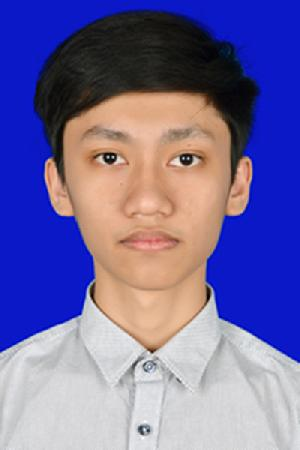
\includegraphics[height=0.3\textheight]{penutup/img/foto.jpeg}
\end{wrapfigure}

Penulis bernama Michael Julian Albertus, putra kedua dari tiga bersaudara yang lahir pada tanggal 2 Juli 1998 di Pekanbaru. Penulis telah mengenyam pendidikan di Sekolah Dasar Mardi Yuana Serang pada tahun 2004 hingga 2006, Sekolah Dasar Palm Kids pada tahun 2006 hingga 2009, Sekolah Dasar Negeri 005 Sukajadi Pekanbaru pada tahun 2009 hingga 2010, Sekolah Menengah Pertama Negeri 5 Pekanbaru pada tahun 2010 hingga 2013, dan Sekolah Menengah Atas Negeri 8 Pekanbaru pada tahun 2013 hingga 2015. Pada masa penulisan, penulis sedang menempuh masa studi S1 di Institut Teknologi Sepuluh Nopember, Surabaya di \jurusan.

Selama masa studi, penulis memiliki ketertarikan yang dalam mengenai \textit{artificial intelligence}, \textit{competitive programming}, dan rancang bangun aplikasi sistem informasi. Keinginan penulis dalam mengajar juga mendorong penulis menjadi asisten dosen pada mata kuliah Dasar Pemrograman, Struktur Data, dan Sistem Operasi. Karya penulis semasa perkuliahan diantaranya adalah pembangunan SheNeedsLab dan LPencerdas untuk acara Hackathon. Selama menempuh perkuliahan penulis juga aktif mengikuti kompetisi pemrograman tingkat nasional dan menjadi finalis pada lomba pemrograman COMPFEST (2017, 2018, dan 2019), INC Bina Nusantara (2017, 2018, dan 2019), FINDIT 2019, Arkavidia (2017,2018, dan 2019) dan menjadi Juara 3 HOLOGY 2018.

Di luar kesibukan akademik, penulis juga berkontribusi dalam berbagai kepanitiaan, baik dalam skala kecil (yaitu dalam kampus) maupun skala nasional. Kepanitian yang penulis ikuti adalah Schematics (2017 dan 2018). Kegiatan terakhir penulis adalah membantu kegiatan pelatihan nasional bagi peserta Olimpiade Komputer Indonesia pada Februari dan Maret 2019 lalu. Penulis dapat dihubungi melalui surel di michaeljulian98@gmail.com.


		
\end{sloppypar}
\end{document}